% % % % % % % % % % % % % % % % % % % % % % % % % % % % % % %
%		Ab hier werden die Dateien eingeladen
% Wenn sich der Name der Datei ändert müsst ihr das hier auch ändern
%% % % % % % % % % % % % % % % % % % % % % % % % % % % % % % %

% Das Professoren-Buchstaben-Bild
\newpage\thispagestyle{plain}
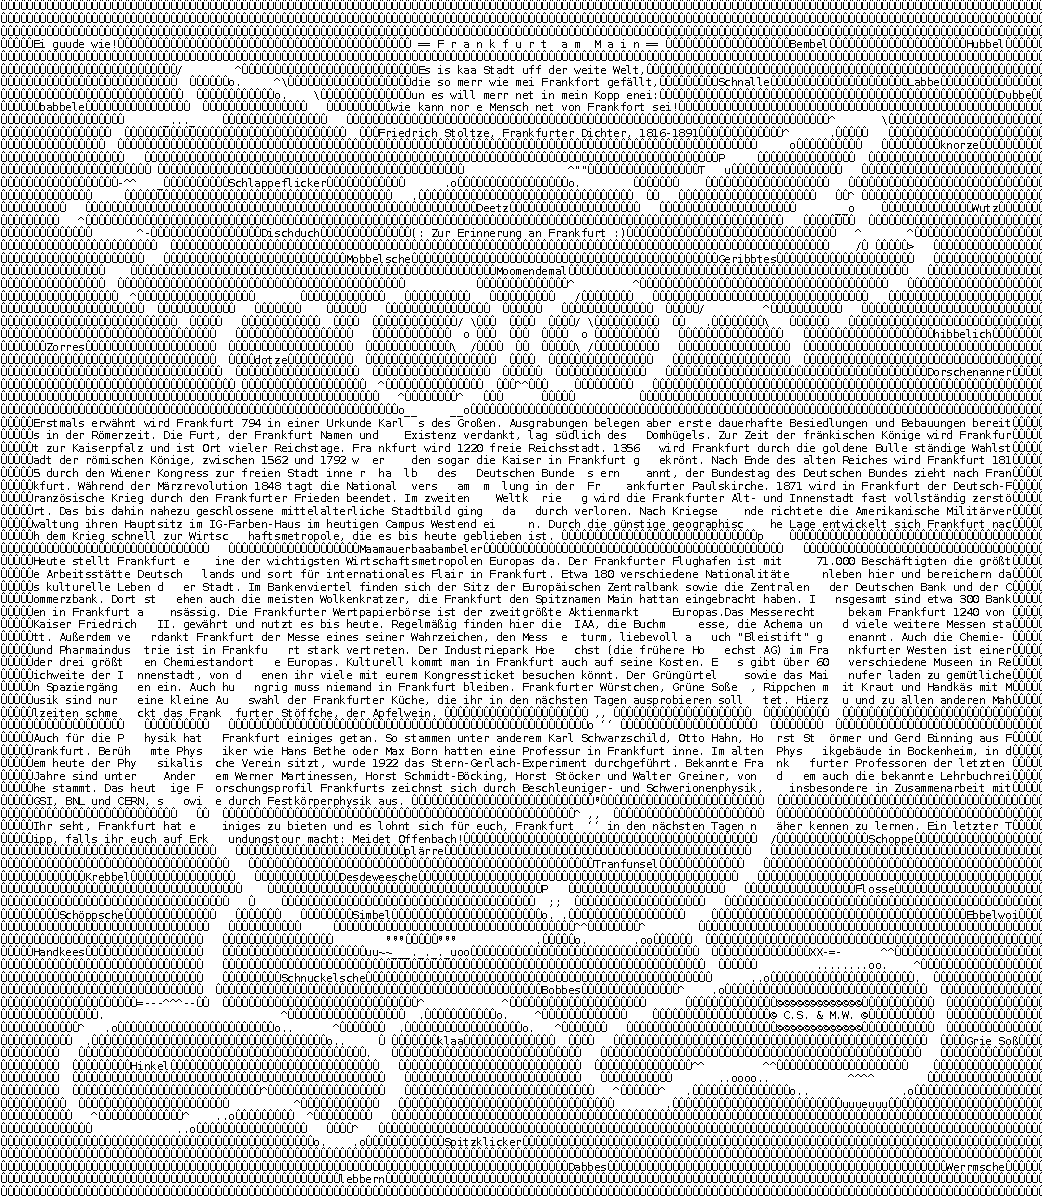
\includegraphics[height=1\textheight,width=1\textwidth]{\imgdir/prof-ffm.pdf}
~%
\newpage
%
% Die eigentlichen Texte
% ab hier Kopf- und Fußzeile
%
\pagestyle{scrheadings}
\section[Die Fachschaft]{Kleine Vorstellung der Fachschaft}
Der erste und wichtigste Anlaufpunkt für euch ist am Anfang des Semesters höchstwahrscheinlich die Fachschaft.
Wir werden euch unterstützen, eure Fragen beantworten und euch bei Problemen bestmöglich beistehen.\\
Ihr werdet euch nun fragen, wer oder was überhaupt diese Fachschaft ist. Die Fachschaft besteht aus einer Gruppe Studierender, die sich über das Studium hinaus noch für ihre Kommilitonen einsetzen und das Studium für aktuelle und zukünftige Studierende so gut wie möglich zu gestalten.\\
Die Frage ist nun: \enquote{Was machen die Fachschaftsmitglieder*innen denn so den ganzen Tag?}\\
Zuallererst gestalten wir zum Beispiel das That's it und die Erstsemestereinführung, um euch den Einstieg ins Studium zu erleichtern, euch kennen zu lernen und uns ein wenig vorzustellen. Da wir uns alle noch sehr gut an die Probleme der ersten Wochen erinnern können, liegt uns das Gelingen dieser Veranstaltung besonders am Herzen. Wir übernehmen aber auch die Organisation des Sommerfestes, der Night of Science und anderer Feierlichkeiten am Fachbereich.\\
Wir befassen uns außerdem noch mit ganz anderen Aufgabenfeldern:
Zunächst sind Fachschaftsmitglieder*innen in mehreren Ausschüssen präsent und vertreten dort die Interessen der Studierenden. Hier sitzen wir mit Professor*innen und wissenschaftlichen Mitarbeiter*innen am Tisch und diskutieren zum Beispiel über Änderungen der Studienordnung, Finanzierung neuer Lehrmittel oder stellen gemeinsam einen Preis für gute Lehre am Fachbereich Physik auf die Beine.\\
Des Weiteren wäre da noch die nicht ganz so einfache Aufgabe der Vermittlung:
Wenn \enquote{Studierendeninteressen} mit denen der Professor*innen kollidieren kann die Fachschaft oft gut vermitteln, da wir seit Jahren einen guten Kontakt zu den Professor*innen pflegen.\\
Wahrscheinlich haben wir nun unzählige wichtige Aufgaben der Fachschaft vergessen, aber ihr merkt schon, dass die Fachschaft das \enquote{Sprachrohr} der Studierenden ist und viele motivierte Studierende sich hier Tag für Tag für euch engagieren.\\
Wenn ihr interessiert seid, mitzumachen, einfach nur Hilfe braucht, um über die Wirren der ersten Wochen hinwegzukommen, oder ihr Rat sucht, dann kommt einfach vorbei. Die Fachschaft besteht aus relativ vielen Vegetariern und auch die anderen fressen selten Erstsemestler, so gut schmeckt ihr nun auch nicht\ldots\\
Uns zu finden ist nicht so schwer und wir freuen uns über Besuch:\\
Hauptgebäude rein\ldots erste Tür links\ldots Gang durchgehen und vor der Glastür an der letzten Tür rechts klopfen. Nebenan findet ihr mit dem Phasenraum eine Möglichkeit euch zum Lernen zurückzuziehen und könnt dort sogar für die Lernpause über die Fachschaft Gesellschaftsspiele ausleihen.\\
Man sieht sich!
\newpage
\begin{figure}
	\centering
	\includegraphics[width=\textwidth]{\imgdir/ernst.JPG}
	\captionsetup{labelformat=empty}
	\caption{
		Auf dem Bild seht ihr die aktuellen Fachschaftsmitglieder (immer von links nach rechts):\\\\
		Vorne: Laura L, Carlotte, Laura S, Frede, Daniela, Zoe, Flo, Laurin\\
		2. Reihe: Kathii, Julii, Bastian, Anja, Nicklas, Magnus\\
		3. Reihe: Jesse, Jan, Lena, Kappa, Clara, Sigrid, Marius, Stefan, Ole\\
		4. Reihe: Fabian, Stephan, Tim, Balu, Martin\\
	}
\end{figure}
\section{Aus dem Leben eines Erstsemesters}
\label{sec:erstsemester_leben}
4:30 Uhr: Der ohrenbetäubende Lärm des Weckers rei\ss t mich aus dem Schlaf. Ich werfe die Bücher beiseite und springe vom Schreibtischstuhl auf. Das war eine erholsame Nacht, ich fühle mich wie neugeboren. Wo ist nur mein Theo-Zettel hin? Ich hab` doch gestern Abend noch bis um 3 dran gearbeitet? Wie jede Nacht. Tag und Nacht!\\
Im Traum ist mir doch glatt die Lösung der verdammt inhomogenen Differentialgleichung 25.ter Ordnung mit frequenzabhängigen Dispersionsrelationen bei nichttrivialen Randbedingungen eingefallen! Und das im Lagrange-Formalismus! Ach, da ist der Theo-Zettel ja. Auf dem Boden. Ich war nicht kräftig genug, den Batzen Papier auf den Schreibtisch zu heben. Au\ss erdem wäre der Tisch sowieso zusammengebrochen. Da rechne ich doch geschwind mal weiter, ich habe ja noch eine halbe Stunde Zeit.\\
5:00 Uhr: Ich treffe mich mit drei Kommilitonen, um die Mathe-Vorlesung vorzubereiten. Heute geht es um die Approximation differenzierbarer Funktionen durch Anwendung des Virialsatzes auf die Säkulardeterminante. Ein spannendes Thema, das man gleich benutzen kann, den Lemaître-Eddington-Kosmos des Reflexklystrons im Lobatschewsky-Bolyai-Raum zu veranschaulichen. Heute wird ein schöner Tag.\\
6:00 Uhr: Zeit für die fünf Protokolle, die ich heute abgeben muss. Eigentlich ist das gemein - fünf Protokolle. Von gestern auf heute. Aber wer damit nicht klar kommt, der gehört hier halt nicht hin. Die Leute findet man dosenstapelnderweise beim Aldi. Oder bei den BWL--ern.\\
7:00 Uhr: Zeit für Frühstück.\\
7:01 Uhr: Ah, jetzt geht`s mir gut. Ab zu den Informatikern, ein Nebenfach will schlie\ss lich auch gepflegt werden. Ich wundere mich ja heute noch wie man vier Programmiersprachen in drei Tagen lernen kann, aber irgendwie ging`s!\\
7:30 Uhr: Ich muss noch die drei Kilo Papier besorgen, die ich für die Vorlesung brauche. Der flei\ss ige Physikstudent schreibt schlie\ss lich mit. Au\ss erdem, ist es Zeit für die tägliche Koffeinspritze.\\
7:45 Uhr: Ab in den Hörsaal, sonst sitz` ich schon wieder nur in der zweiten Reihe. Juhu, diesmal hab ich noch einen Platz in der ersten Reihe ergattern können, ein bisschen am Rand, aber die anderen waren einfach schon `ne Stunde früher als ich.\\
8:15 Uhr: Der Messias betritt den Saal. Er erleuchtet uns die
folgenden zwei Stunden mit reinstem, gesegnetem Wissen\ldots\\
10:15 Uhr: Experimentalphysik. Das finde ich langweilig, weil
trivial.\\
11:15 Uhr: Eine Freistunde! Heissa! Endlich kann ich in Ruhe ganz alleine rechnen. Ich hab doch gesagt, dass ein schöner Tag wird! Ich versteh nicht, wie andere essen gehen können. Was soll das? Stümper\ldots\\
12:15 Uhr: Theoretische Physik, die Königin der Wissenschaften. Hier ist man Gott am nächsten! Alle gucken so verwirrt, als ob sie es nicht verstanden hätten. Dabei sind wir doch erst bei Seite 798 des Buches, und es sind erst zwei Wochen rum. Wie können die eigentlich die täglichen fünfzehn Aufgaben schaffen, wenn sie nicht mal die Vorlesung verstehen? Oder vielleicht schauen sie auch nur gelangweilt. Ich muss auch zugeben, eine Geschwindigkeit von einer Tafel in zwei Minuten ist schon etwas lahm. Der war auch mal schneller.\\
13:00 Uhr: Fachbereichsratssitzung. Etwas politisches Engagement wird von einem Erstsemester schlie\ss lich auch erwartet.\\
22:30 Uhr: Nach einem Diskussionsmarathon darüber, ob Professor Greiner wegen seines neuen Ehrendoktors heute den Platz am Kopfende des Tisches bekommt oder doch neben dem Aquarium sitzen muss, mussten wir mangels einer alle zufrieden stellenden Lösung die Sitzung vorzeitig beenden. Glücklicherweise, denn sonst hätte ich nicht die Zeit gefunden, das Buch \enquote{Corund methods for the solution of the cyropolus-problem with the leptonic Purcell-Planck-equation} durchzulesen, das ich doch für die Aufgaben brauche.\\
23:30 Uhr: Puh, geschafft. Wenn man wöchentlich ein Bibliotheksregal durcharbeiten muss, lernt man das schnelle Lesen ganz gut. Jetzt muss ich aber wirklich meine Theo-Aufgaben weiter rechnen!\\
4:30 Uhr: Zeit zu schlafen, leider, aber was sein muss, muss sein.\\
4:45 Uhr: Endlich, ein neuer interessanter, spannender, aufregender Physiker-Tag beginnt\ldots
\begin{figure}[!b]
 	\centering
  	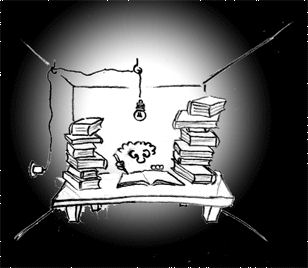
\includegraphics[width=.8\textwidth]{\imgdir/ersti.jpg}
\end{figure}
\von{Sascha (der hat jetzt seinen 20. Herzinfarkt hinter sich\ldots) und Julia}
\section{Stundenplan}

Alles schön und gut, in Wirklichkeit interessiert euch doch vornehmlich eines: Wie sieht euer Studium denn nun aus und was müsst ihr vor Beginn des Semesters tun. Damit legen wir jetzt los:

Hier seht ihr ihn, vielleicht zum ersten Mal: Euren Neuen und ganz persönlicher Stundenplan. Im ersten Moment kommt er euch vielleicht noch sehr leer vor, wenn ihr ihn mit eurem Stundenplan aus der Oberstufe vergleicht.
Lasst euch davon nicht täuschen, denn dieser Stundenplan mutiert wenn ihr nicht aufpasst schnell zu einem Zeit- und soziale Kontakte- fressenden schwarzen Loch. Denn statt Hausaufgaben habt ihr neben Vorlesungen und Übungen in den Grundvorlesungen Übungszettel, die es zu bearbeiten und abzugeben gilt um die Klausurzulassung zu erreichen, was schnell in zeitintensive Nachbereitung der Vorlesung und Recherche ausartet und mit gewohnten Hausaufgaben wirklich nichts mehr zu tun hat.

Euer Stundenplan besteht zusammengefasst aus Vorlesungen, Tutorien und der unsichtbar bleibenden Zeit für Übungszettel. 
Da ihr euer Studium im Sommersemester beginnt werdet ihr in eurem ersten Semester nur Vorlesungen aus dem Bereich der Theoretischen Physik mit mathematischer Ergänzung und der Experimentalphysik sowie ggfs. ein Nebenfach belegen. Die 
\glqq echte\grqq  Mathematik beginnt ihr dann in eurem zweiten Semester, trotzdem solltet ihr euch zum Verständnis der theoretischen Physik zumindest in der Vorlesung \glqq Mathematische Ergänzung zur theoretischen Physik\grqq   bereits ausführlich damit auseinander setzen. 

Vorlesungen gehen jeweils über 2 Stunden und es besteht keine Anwesenheitspflicht. Lasst euch davon aber nicht täuschen, denn wenn ihr es ernst mit dem Studium meint kommt ihr um den Besuch der Vorlesung kaum herum. Es ist zwar schwer, dem Menschen an der Tafel zu folgen, noch viel schwerer ist es aber, den Vorlesungsstoff für die Übungsaufgaben und die Klausur komplett eigenständig zu erarbeiten. Vor Allem könnt ihr den Profs in den Vorlesungen Fragen stellen, wohingegen die meisten Bücher einen daraufhin nur hämisch anschweigen oder auf der nächsten Seite darauf verweisen, dass dies \glqq offensichtlich\grqq   aus Satz 193b.IV des Buches \glqq Quantenchromoelektrodynamik für Fortgeschrittene\grqq   folge. Dann doch lieber 2 Stunden Vorlesung.

Um das was in der Vorlesung theoretisch in euer Gehirn eingeflößt wurde mal praktisch angewendet zu haben sowie zur Nachbesprechung der Übungszettel habt ihr sogenannte Tutorien. Hier ist die Anwesenheit (bis auf wenige Ausnahmen) Pflicht, ebenso die aktive Beteiligung durch Mitarbeit und Vorrechnen an der Tafel. Oft ist das Tutorium aber auch der Ort, wo man beginnt, wirklich zu verstehen was das alles soll, denn hier steht euch ein*e Student*in aus höheren Semestern, ein*e Masterstudent*in oder ein*e Doktorand*in zur Seite, hat Zeit, wirklich auf Fragen einzugehen und weiß oft noch von sich selbst oder aus anderen Tutorien, welche Knoten es in den Denkmuskeln zu lösen gilt, welche Methoden wirklich hilfreich zum Verständnis sind und können euch so den Weg zur erfolgreichen Klausur und zum Verständnis sehr erleichtern. Tutorien werden in der Woche zu vielen verschiedenen Terminen angeboten, die genauen Termine werden euch die Professoren oder Übungsleiter in der ersten Vorlesung bekannt geben, zusammen mit den notwendigen Informationen zur Anmeldung.

Die letzte Veranstaltung, die noch in Eurem Stundenplan steht ist das physikalische Kolloquium, bei dem es nicht nur Kaffee und Kekse gibt, sondern auch interessante Vorträge über die aktuelle Physik. Auch wenn ihr aktuell vielleicht noch nicht so viel versteht, spannend ist es trotzdem zu sehen, was es so alles gibt und ihr werdet staunen, wie schnell euch diese seltsamen Zeichen an der Tafel anfangen, bekannt vor zu kommen. Es geht kaum etwas über die Freude, im zweiten Semester eine Methode auf einmal wie selbstverständlich anzuwenden, die einen im ersten Semester noch zur Verzweiflung gebracht hat. 

Wenn euch das jetzt nicht zu sehr abgeschreckt hat und ihr immer noch Lust auf euer Physikstudium für Masochisten habt: viel Spaß beim Lesen eures Stundenplans. Die Informationen, wie und ob man sich für Fächer, Klausuren und Co anmelden müsst erhaltet ihr von uns bei der Erstsemester-Einführung.

\newcommand{\rb}{\raisebox{-1.5ex}[-1.5ex]}

\noindent%%%%%%%%%%%%%%%%%%%%%%%%%%%%Physik%%%%%%%%%%%%%%%%%%%%%%%%%%%%
\

\begin{sideways}
\begin{minipage}{1\textheight}
%\begin{tabular}{|c||c|c|c|c|c|}\hline
\center \textbf{\Large Stundenplan für Bachelor Physik}\bigskip\\
\begin{tabular}{|p{.05\textheight}||p{.16\textheight}|p{.16\textheight}|p{.16\textheight}|p{.16\textheight}|p{.16\textheight}|}\hline
 Zeit 		& Montag 			& Dienstag 			& Mittwoch 		& Donnerstag 		& Freitag	\\ \hline\hline
{08.00} 	& 					&					&  {Ex 2}		& {Theoretikum} 	&  			\\ 
&&&&&\\ \cline{1-3} \cline{6-6}
{09.00} 	& 					&					&  {OSZ H1}		& {!!! Beispiel !!!}&			\\
&&&&&\\ \cline{1-6}
{10.00} 	& 	 				&  					& {Theo 1/2}	& 					& {Ex 2}	\\
&&&&&\\ \cline{1-3}\cline{5-5}
{11.00} 	& 	 				& 					& {\_0.111} 	&  {Theo 1/2}		& {OSZ H1}	\\
&&&&&\\ \cline{1-4} \cline{6-6}
{12.00} 	& 					& {Theo 1/2}		& 	 			& {\_.102}			& 			\\
&&&&&\\ \cline{1-2} \cline{4-6}
{13.00} 	&					& 	{\_.102}		& 				& 					&  			\\
&&&&&\\ \hline 
{14.00} 	& {Mathe Ergänzung} &{Übung Ex 2}		& 				&  					& 			\\
&&&&&\\ \cline{1-1}  \cline{4-6}
{15.00} 	& {OSZ H1}	 		&{!!! Beispiel !!!}	& 				&	  				& 			\\
&&&&&\\ \hline
 {16.00} 	&  					&  					& {Kolloquium} 	&  					& 			\\
&&&&&\\ \cline{1-3} \cline{5-6}
 {17.00} 	&  					&  					& {\_0.111} 	&  					& 			\\
&&&&&\\ \hline 
 {18.00} 	&  					&	  				& 		 		&		  			& 			\\
&&&&&\\ \hline
 {19.00} 	&  					&  					&  				& 					& 			\\
&&&&&\\ \hline
\end{tabular}
\end{minipage}
%}
\end{sideways}
%
%
%\noindent%%%%%%%%%%%%%%%%%%%%%%%%%Biophysik%%%%%%%%%%%%%%%%%%%%%%%%%%%%
%\
%
%\begin{sideways}
%\begin{minipage}{1\textheight}
%\center \textbf{\Large Stundenplan für Bachelor Biophysik}\bigskip\\
%\begin{tabular}{|p{.05\textheight}||p{.16\textheight}|p{.16\textheight}|p{.16\textheight}|p{.16\textheight}|p{.16\textheight}|}\hline
% Zeit 		& Montag 	& Dienstag 	& Mittwoch 	& Donnerstag 	& Freitag \\ \hline\hline
%{08.00} 	&  		&  		& {Ex 2}  	&  		&		\\ 
%&&&&&\\ \cline{1-3} \cline{5-6}
%{09.00} 	&  		&  		& {OSZ H1}	& {Theo 1} 	&		\\
%&&&&&\\ \cline{1-4} \cline{6-6}
%{10.00} 	& 	 	& {Theo 1/2} 	& {Ex -- Übung}	& {\_0.111} 	& 		\\
%&&&&&\\ \cline{1-2} \cline{5-6}
%{11.00} 	& 	 	& {\_0.111}	& {!!! Beispiel !!!} & {Ex 2} 	& 		\\
%&&&&&\\ \cline{1-4} \cline{6-6}
%	{12.00} 	& {Theoretikum}	&  		& {Theo 1/2} 	& {OSZ H1} 	& {Mathematik für Biophysiker} \\
%&&&&&\\ \cline{1-1} \cline{3-3} \cline{5-6}
%	{13.00} 	& {!!! Beispiel !!!} & 		& {\_0.111} 	& {Mathe-Übung !!!Beispiel!!} & {\_\_.401} \\
%&&&&&\\ \hline 
%{14.00} 	& {Mathe Ergänzung} & 		& 		&  		& 		\\
%&&&&&\\ \cline{1-1} \cline{3-6}
%{15.00} 	& {\_0.111}	 &  		& 		&	  	& 		\\
%&&&&&\\ \hline
% {16.00} 	&  		&  		& {Kolloquium} 	&  		& 		\\
%&&&&&\\ \cline{1-3} \cline{5-6}
% {17.00} 	&  		&  		& {\_0.111} 	&  		& 		\\
%&&&&&\\ \hline 
% {18.00} 	&  		&  		&  		&  		& 		\\
%&&&&&\\ \hline
% {19.00} 	&  		&  		&  		&  		& 		\\
%&&&&&\\ \hline
%\end{tabular}
%\end{minipage}
%%}
%\end{sideways}

\section{How to Veranstaltungen und Prüfungen}
\subsection{Den Stundenplan selbst erstellen}
Jetzt haben wir euch zwar schon einen wundervollen Stundenplan zusammengestellt, vielleicht habt ihr aber Lust, noch ein Nebenfach zu belegen, wollt doch lieber mit theoretischer Physik 4 anfangen (das ist keine Empfehlung!) oder fragt euch, wie man sich zu diesen Fächern denn nun anmeldet. So oder so werdet ihr spätestens im nächsten Semester selbst verantwortlich dafür sein, die richtigen Veranstaltungen zusammen zu suchen. Hierzu werdet ihr zwei Instrumente besonders brauchen:\\
Zuallererst und insbesondere benötigt ihr das \textbf{Modulhandbuch} eures Studienganges. Dieses findet ihr, ebenso wie die Prüfungsordnung, auf der Homepage des Prüfungsamtes (\url{https://www.uni-frankfurt.de/60644473/Pruefungsamt}, wobei sich die wenigsten erfahrenen Studenten durch die Uni-Seiten klicken sondern einfach die Suchmaschine ihrer Wahl bemühen). Beide Dokumente solltet ihr in jedem Falle mal gelesen haben, denn hier stehen die wichtigsten Informationen zu eurem Studium. So findet ihr im Modulhandbuch ausführlich eine Beschreibung zu jedem angebotenen Modul (\fach{Fach} das ggfs. aus mehreren verschiedenen Vorlesungen oder Veranstaltungen bestehen kann), dessen Inhalte, benötigte Vorkenntnisse und einer Empfehlung, in welchem Fachsemester es zu belegen ist. Ihr braucht euch an diese Empfehlung nicht zu halten und in vielen Fällen ist dies mit einem Studienbeginn im Sommersemester auch gar nicht möglich, es gibt euch aber einen guten Überblick. Damit ihr wisst, in welcher Reihenfolge die Fächer für euch gedacht sind, erhaltet ihr auf der Erstsemester-Einführung noch einen Studiengangplan für den Studienbeginn im Sommersemester. Mit den nun erlesenen Informationen geht es jetzt weiter auf \url{qis.server.uni-frankfurt.de}, denn dort befindet sich das \textbf{Vorlesungsverzeichnis}.\\
Bei der Abholung eurer Goethe-Card solltet ihr einen Benutzernamen für euren HRZ-Account sowie per Post ein Passwort erhalten haben. Mit diesen könnt ihr euch im QIS einloggen und ab sofort könnt ihr den Großteil eurer Uni-Formalitäten hier regeln. Zur Erstellung eines Stundenplans geht es weiter über \fach{Veranstaltungen} und \fach{Vorlesungsverzeichnis}, hier muss man sich ein bisschen durchklicken, bis man den richtigen Fachbereich (13), den richtigen Studiengang (z.B. Bachelor \fach{Physik}) und den passenden Studienabschnitt (z.B. \fach{gemeinsame Pflichtveranstaltungen}) eingestellt hat. So kommt man letztendlich zur Fachübersicht, wo ihr alle Pflichtvorlesungen, Übungen, Ergänzungskurse etc. zu allen Pflichtveranstaltungen aufgelistet seht, die in diesem Semester angeboten werden. Zum Glück braucht ihr ja nicht alle in einem Semester belegen sondern sucht euch einfach diejenigen zusammen, für die ihr euch mit dem Modulhandbuch entschieden habt. Auf den einzelnen Unterseiten seht ihr nun noch einmal verschiedene Informationen zu den Veranstaltungen, insbesondere an welchem Wochentag und zu welcher Uhrzeit sie angeboten werden. Hierbei gilt es vorsichtig zu unterscheiden zwischen mehreren festen Terminen die Woche (meist bei Vorlesungen), einem festen einmaligen Termin (z.B. Einführungsveranstaltungen) oder vielen Optionen von denen am Ende eine gewählt werden soll (häufig bei Übungen). \\
Zur Übersicht kann man sich die festen Termine vom QIS in einen Stundenplan zusammentragen oder für Outlook exportieren lassen. Für den Export klickt ihr auf der Veranstaltungsseite auf das Kalendersymbol neben dem jeweiligen Termin. Für die Erstellung eines Stundenplans im QIS markiert ihr die Termine und klickt auf \fach{markierte Termine vormerken}. Ihr werdet dann auf einen Stundenplan weitergeleitet, in dem alle in dieser Sitzung vorgemerkten Termine angezeigt werden. Wenn ihr ihn dauerhaft speichern wollt könnt ihr oben auf \fach{Plan speichern} klicken. Es erscheint nun eine Warnung, dass die Veranstaltungen nur vorgemerkt, aber nicht belegt sind.
%
%
\subsection{Belegen von Veranstaltungen}
Im Fachbereich 13 gibt es für \textbf{Vorlesungen} im Allgemeinen keine Belegpflicht. Ihr braucht also nur die passenden Termine im Vorlesungsverzeichnis zusammentragen, damit ihr wisst, wann ihr wo sein müsst (wollt), könnt dann aber einfach zu den Vorlesungen kommen ohne das irgendwo anzumelden. Dies gilt nicht zwingend auch für Nebenfächer oder Fächer, die von anderen Fachbereichen angeboten werden, bei Nebenfächern also immer lieber mal nachfragen. \\
Bei \textbf{Übungen} wird meistens in der ersten Vorlesung erklärt, wie die Anmeldung abläuft, hier gibt es verschiedene Plattformen, verschiedene Zuteilungsmethoden, manche Professoren nutzen hierfür Plattformen wie das elearning-Portal, andere ihre eigene Website oder Zettel an der Tür des Büros. Die Anmeldung ist hier im Allgemeinen Pflicht und oft sollte diese auch möglichst schnell erfolgen, wenn man einen begehrten Termin ergattern möchte. In den höheren Semestern sind sie manchmal sogar schon vor Beginn der Vorlesungszeit freigeschaltet, die Frist endet aber immer erst nach den ersten Vorlesungen, also keine Angst. \\
Etwas mehr aufpassen muss man da bei den für euch ab dem 2. Semester relevanten \textbf{Praktika}, denn deren Anmeldung läuft tatsächlich schon vor Beginn des nächsten Semesters aus. Alle Informationen zur Anmeldung und zu den Anmeldefristen findet ihr auf der Seite des Anfängerpraktikums (\url{https://www.uni-frankfurt.de/44824371/A_Praktikum}).
%
%
\subsection{Prüfungsanmeldung}
Studieren schön und gut, eines Tages ist es soweit und auch das entspannteste Fach endet meist mit einer Prüfung. Da ihr euch zu der Vorlesung ja schon gar nicht angemeldet habt, kann euch niemand dazu zwingen, die Prüfung jetzt mit zu schreiben. Im Fachbereich 13 gibt es jedoch den sogenannten \fach{Freiversuch}, wenn ihr also eine Prüfung im ersten dafür vorgesehenen Semester schreibt, zählt sie bei Nichtbestehen nicht als Fehlversuch (\S 34 Prüfungsordnung 2013). Es ist also doch empfehlenswert, die Prüfung nun auch zu schreiben und dafür muss man sich, im Gegensatz zu den Vorlesungen, anmelden. Damit ihr euch anmelden dürft wird der Prof euch zu Beginn des Semesters darüber informieren, welche Voraussetzungen es zu erfüllen gilt (Teilnahme an Übungen, bestimmte Punkteanzahl in den Übungsblättern und ähnliches). Wenn ihr dann gegen Ende des Semesters alles so weit geschafft habt, sind sich die Profs häufig nicht ganz einig, wie man sich denn zu den Prüfungen anmelden soll. Dies ist in der Physik zentral geregelt und passiert ausschließlich über das QIS unter \fach{Prüfungsverwaltung} (haltet eure Tan-Liste bereit). Die Anmeldung ist in den Grundvorlesungen im Allgemeinen bis 1 Woche vor der Prüfung möglich, wer sich dann doch wieder abmelden möchte kann dies bis einen Tag vor der Prüfung ebenfalls im QIS tun. Sollte es Probleme dabei geben könnt ihr euch mit euren Fragen an die netten Damen vom Prüfungsamt wenden. \\
\par 
So, jetzt solltet ihr das Wichtigste zum Studieren wissen. Wenn ihr noch Fragen habt steht euch die Fachschaft jederzeit gerne zur Verfügung. Viel Erfolg! 
\von{Frederike}
\section{Studienstruktur}

\subsection{Bachelor in Physik}
\bigskip
%
Glücklicherweise seid ihr nicht mehr die ersten, die in Frankfurt auf Bachelor studieren.
Ab dem letzten Semester gibt es einen neuen, überarbeiteten Studiengang Physik.
Ihr könnt also von den Erfahrungen der vergangenen Semester profitieren.
Der alte Studiengang BSc. Physik wurde nämlich im Wesentlichen beibehalten und an einigen Stellen verbessert.
\bigskip

Innerhalb der sechs Semester bis zum Bachelor müsst ihr viele Veranstaltungen besuchen; was in welchem Semester dran kommt, soll
euch die folgende Aufstellung zeigen. Akut wichtig ist natürlich erstmal euer


\subsubsection{Erstes Semester}
In eurem ersten Semester sollt ihr mindestens drei Vorlesungen besuchen:
\bigskip

In der \fach{Experimentalphysik} kommt die Vorlesung \VL{Experimentalphysik 2: Elektrodynamik},
die das Modul \Modul{VEX2} bildet, auf euch zu.
Die Vorlesung werdet ihr gemeinsam mit den Studierenden hören, die ihr Studium im letzten Wintersemester begonnen haben.
Dies stellt aber kein Problem dar, da diese Vorlesung keine besonderen Vorkenntnisse benötigt werden.
Dieses Modul bringt 8 CP's und ihr müsst dafür eine Klausur schreiben.
\bigskip

Ob es für euch sinnvoll ist, jetzt schon ein \fach{Nebenfach} zu belegen,
hängt davon ab, welches ihr nehmen wollt.
Seht hierzu den Abschnitt ab Seite \pageref{Nebenfach} über Nebenfächer.
\bigskip

Um euer Studium zügig voranzutreiben, ist es sinnvoll, eines der Anfängerpraktika in den ersten beiden Semestern abzuschließen.
Wir empfehlen euch, mit dem \VL{AP 2} zu beginnen, da ihr zuerst die Vorlesung \VL{Elektrodynamik} hört und das \VL{AP 2} auf diese Themen ausgerichtet ist. Ihr könnt es entweder jetzt schon machen oder als Blockpraktikum in der vorlesungsfreien Zeit vor dem Wintersemester oder auch im Wintersemester. Da die Plätze in den Praktika aber nicht ausreichen, ist es sehr üblich und auch normal,
dass die Hälfte eines Jahrgangs zuerst in das \VL{AP 1} geht. Die Praktika, die ihr im ersten bis dritten Semester hinter euch bringen solltet, bilden die Module \Modul{PEX1} und \Modul{PEX2}. Die Studienleistungen hierzu sind eure Protokolle, die Module sind \textbf{unbenotet}.
Wieviele Versuche und Protokolle von euch verlangt werden, hängt von der Länge des Semesters ab.
Praktika werden in Zweier--Gruppen bestritten.

\pagebreak

\subsubsection{Zweites Semester}\label{PhyBa2}
In der \fach{Experimentellen Physik} besucht ihr nun die Vorlesungen \Modul{VEX1A} \VL{Mechanik} und \Modul{VEX1B} \VL{Thermodynamik}.
Diese zwei Veranstaltungen sind so auf das Semester verteilt, dass ihr bis zu den Weihnachtsferien im Dezember die Vorlesung Mechanik besucht und ab Januar die Vorlesung Thermodynamik. Es handelt sich dabei um zwei einzelne Module; über Mechanik schreibt ihr keine Klausur, dafür am Ende des Semesters über Thermodynamik.
\bigskip

Eure theoretische Physikvorlesung behandelt in diesem Semester die \VL{Mathematische Methoden der Theoretischen Physik}. Es gibt 8 CP's für das Modul \Modul{VTH1}.

Im zweiten Semester beginnt ihr mit eurem dritten Haptfach \fach{Mathematik}.
Ihr werdet zusammen mit den Wintersemester--Anfängern die Vorlesung \VL{Mathematik für Studierende der Physik 1} aus dem Modul \Modul{VMATH1} hören, die 8 CP's bringt und mit einer Klausur abgeschlossen wird.
\bigskip

Im Wintersemester kann man die meisten Nebenfächer beginnen. Wenn ihr im ersten Semester noch kein \fach{Nebenfach} gewählt habt, ist nun der richtige Zeitpunkt, eins zu belegen.

\subsubsection{Drittes Semester}
In der Experimentalphysik sind in diesem Semester zwei Vorlesungen vorgesehen, die die Module \Modul{VEX4A} und \Modul{VEX4B} bilden.
Die Vorlesungen behandeln \VL{Kernphysik} und \VL{Festkörperphysik}, bringen jeweils 4 CP und werden am Ende des Semesters einzeln abgeprüft.
\bigskip

In \fach{Theo} ist es die \VL{Mechanik}, die ihr besuchen müsst.
Es handelt sich wieder um eine Vorlesung über 8 CP, die am Ende des Semesters durch eine Klausur abgeprüft wird.
\bigskip

In der Mathematik hört ihr die Vorlesung \VL{Mathematik für Studierende der Physik 2} aus dem Modul \Modul{VMATH2}, die ebenfalls 8 CP's bringt und mit einer Klausur abgeschlossen wird.
\bigskip

Im dritten Semester absolviert ihr nun euer zweites Anfängerpraktikum, entsprechend der Wahl im 2. Semester also das \VL{AP 1} oder \VL{AP 2}.
Jedes der \fach{Praktika} bringt euch 8 unbenotete CP's.

\begin{figure}[p]
  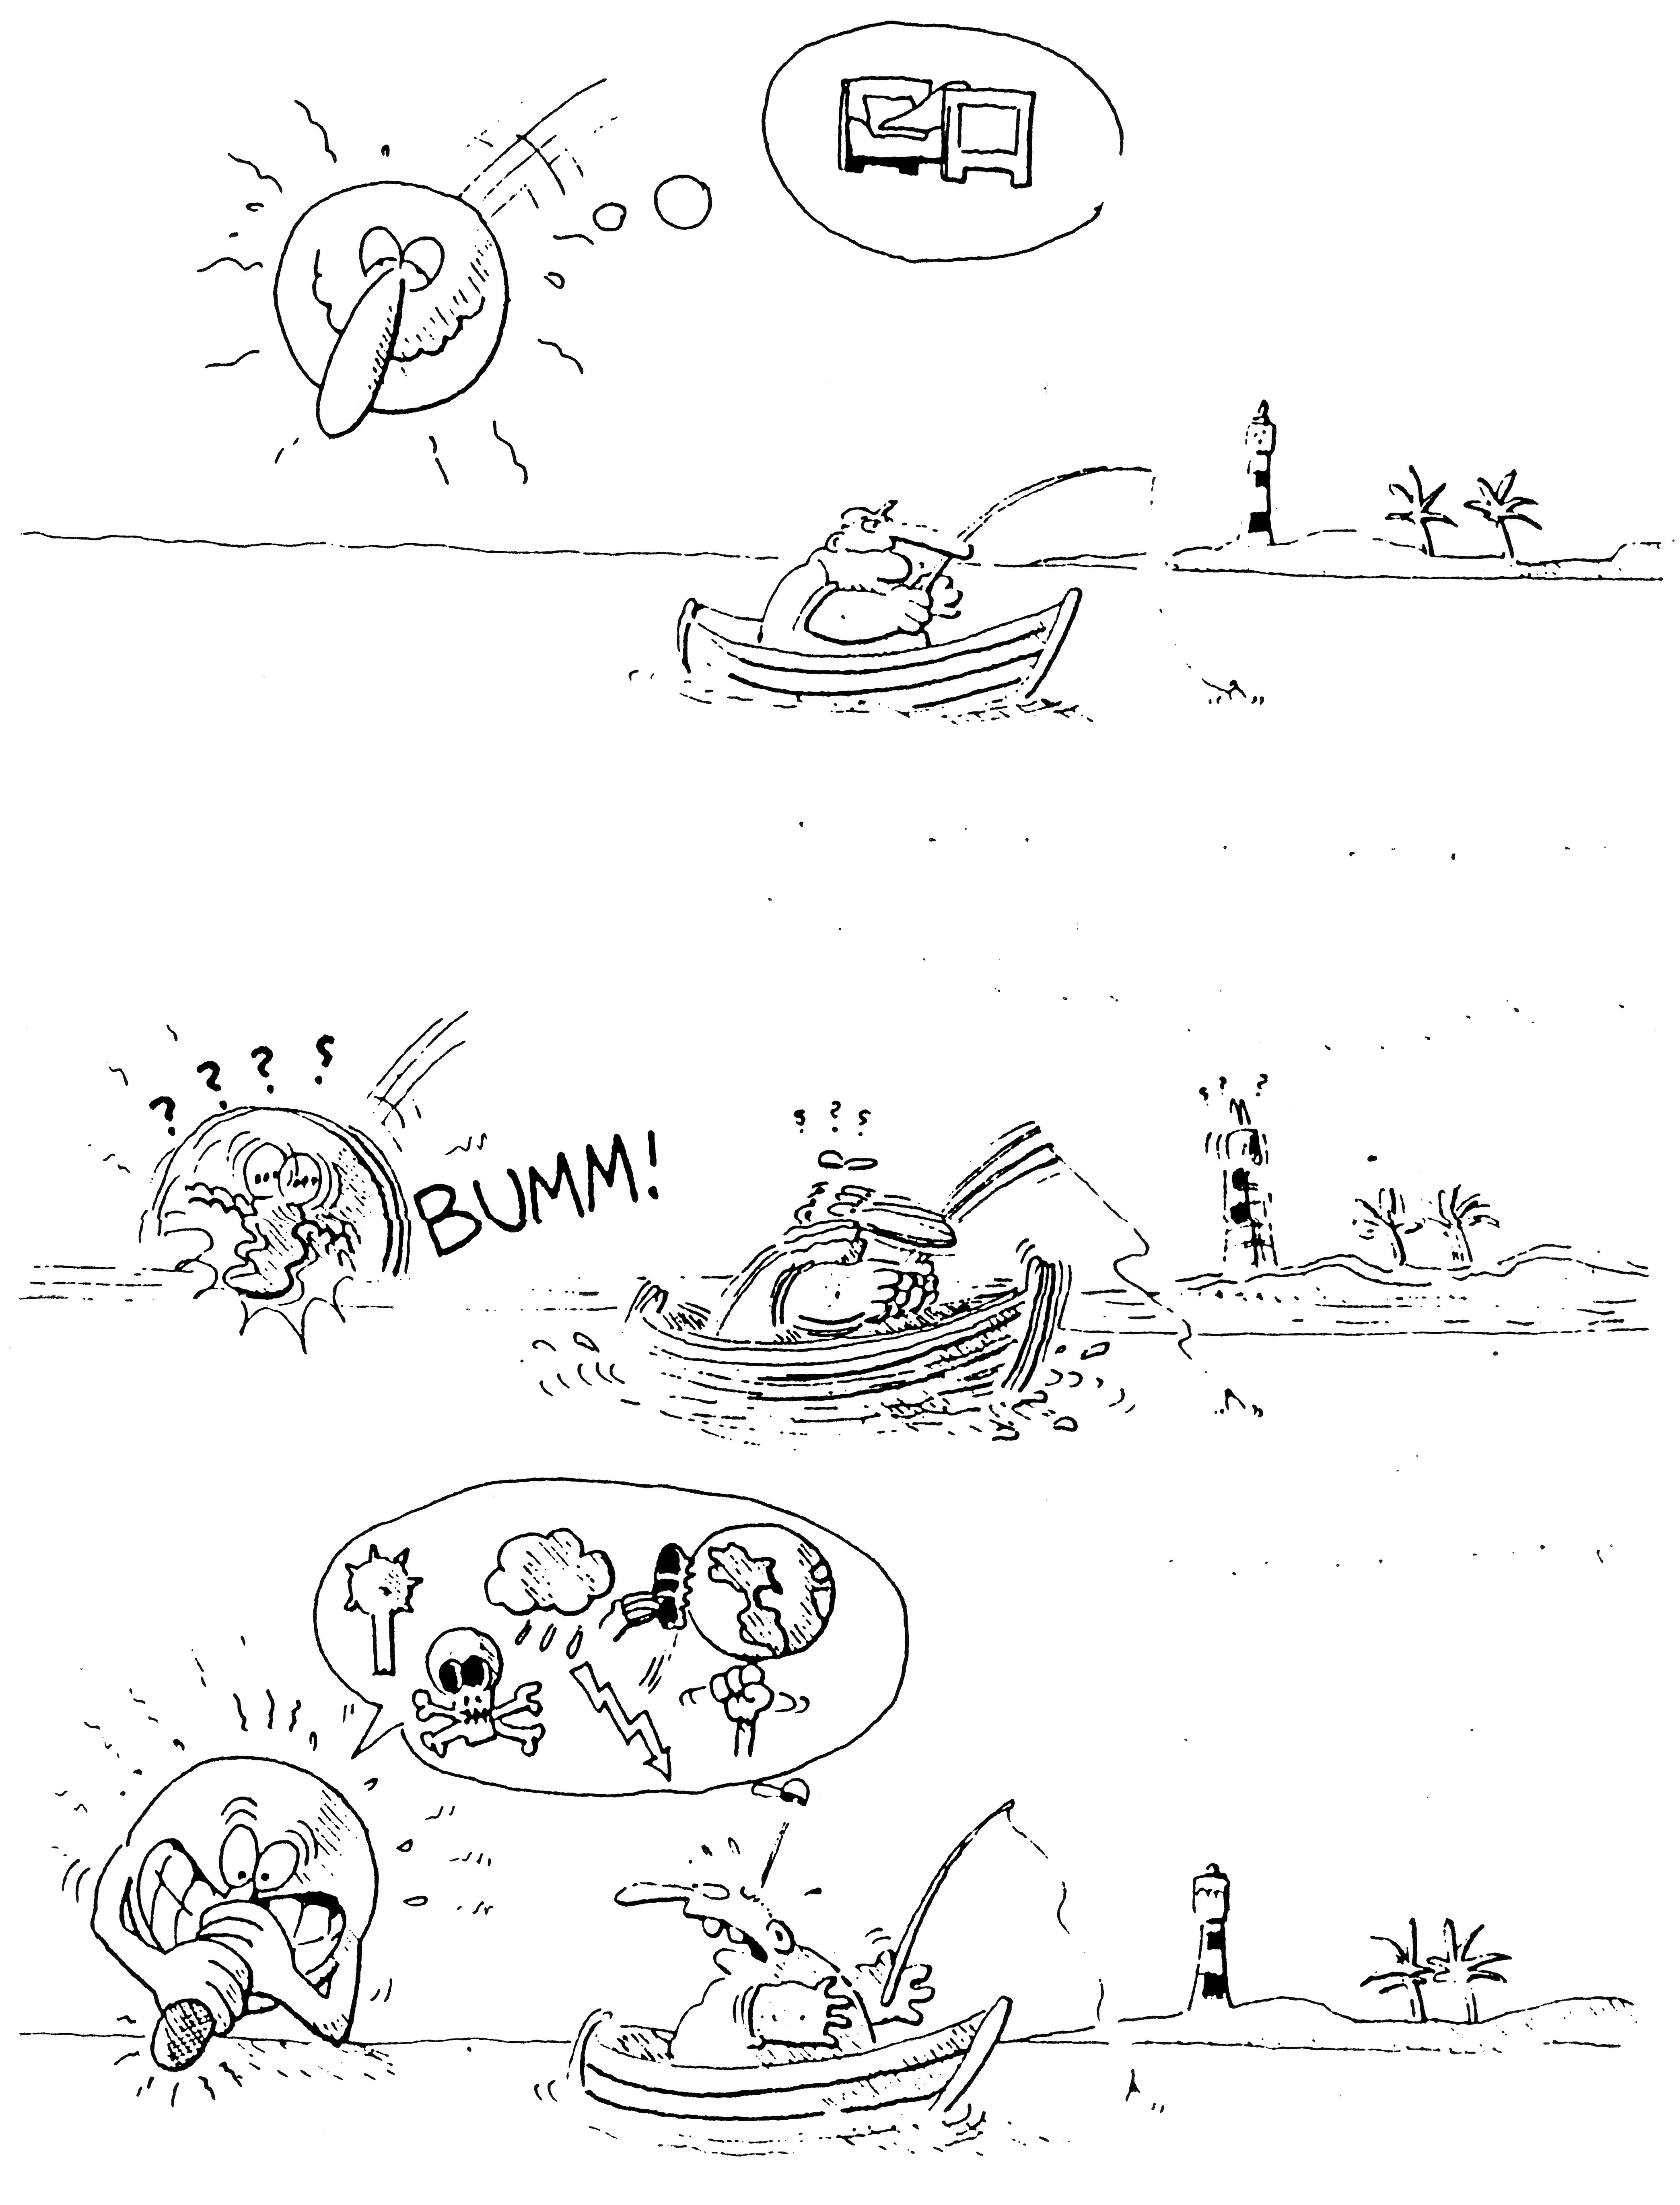
\includegraphics[height=\textheight]{bilder/sonnendotz.jpg}
\end{figure}

\subsubsection{Viertes Semester}

Im vierten Semester steht wieder ein \fach{Praktikum} auf dem Programm, das \VL{Pro\-grammier\-praktikum}, in dem ihr für Physiker wichtige Programmierkenntnisse erlernt (Modul \Modul{PPROG}, 4 CP). Auch dieses Praktikum ist unbenotet
\bigskip

Für dieses Semester sind in der Experimentalphysik zwei Vorlesungen vorgesehen, die zusammen das \Modul{VEX3} bilden. Die Vorlesungen behandeln \VL{Optik} und \VL{Atomphysik}, bringen jeweils 4 CP und werden am Ende des Semesters in einer gemeinsamen Modulabschlussklausur geprüft.

Eure Mathematikausbildung schließt ihr nun mit der Vorlesung \VL{Mathematik für Studierende der Physik 3} ab.
Das Modul \Modul{VMATH3} bringt nach Bestehen einer Klausur auch 8 CP's.
\bigskip

Auch in der \fach{Theoretischen Physik} steht in diesem Semester die \VL{Elektrodynamik} an, die wiederum 8 CP's zählt und mit einer Klausur abgeprüft wird.
\bigskip

Langsam solltet ihr mit den \Modul{Wahlpflichtveranstaltungen}\label{Wahlpflicht} anfangen.
Hier könnt ihr aus einer Vielzahl von Veranstaltungen wählen (manche sind aber erst ab dem fünften Semester geeignet),
ihr müsst insgesamt zwischen 10 und 16 Credit Points (das sind etwa 3-5 Vorlesungen) nachweisen. Jede Veranstaltung wird, wenn überhaupt, einzeln geprüft. Wahlpflicht- und Nebenfachbereich zusammen ergeben ungefähr 19~\% der Bachelor-Endnote.
\bigskip

Die Wahlpflichtveranstaltungen sollen euch Gelegenheit bieten, euch in den einzelnen Arbeits- und Forschungsbereichen
umzuschauen und die Auswahl für euer Arbeitsgebiet in der Bachelor-Arbeit einzugrenzen oder zu treffen.

\subsubsection{Fünftes Semester}

Langsam wird es ernst, eure letzten Praktikum läuft. Es ist das \VL{Fort\-ge\-schri\-tten\-en-Prak\-ti\-kum}, in dem ihr ähnlich wie im Anfängerpraktikum Versuche durchführen und Protokolle abgeben müsst (Modul \Modul{PEXF}, 12 CP).

In der \fach{Theoretischen Physik} wird in diesem Semester ie \VL{Quantenmechanik} behandelt, die wiederum 8 CP's zählt und mit einer Klausur abgeprüft wird.
\bigskip

Außerdem habt ihr in diesem Semester viel Zeit für Wahlpflicht und Nebenfach.

\subsubsection{Sechstes Semester}
Das sechste Semester sollte für die Bachelor-Arbeit zur Verfügung stehen. Jedoch werdet ihr auch noch in der \fach{Theoretischen Physik} die  \VL{Thermodynamik und Statische Physik} behandeln, die wiederum 8 CP's zählt und mit einer Klausur abgeprüft wird.
\bigskip

Hier sollt ihr noch ein Seminar besuchen - das im Regelfall das Arbeitsgruppen-Seminar sein wird,
in der ihr die Bachelor-Arbeit macht.
Einige Wahlpflichtveranstaltungen sind noch für das sechste Semester vorgesehen.
\bigskip

Das Seminar ist nicht benotet, und die Bachelor-Arbeit ergibt
11,8~\% der Gesamtnote.

\paragraph{Anmerkung:} Zur Feststellung der Noten wird folgendes System verwendet:

In der Experimentalphysik schreibt ihr fünf Klausuren
(\VL{Thermodynamik}, \VL{Elektrodynamik}, \VL{Atomphysik und Optik}, \VL{Kernphysik}, \VL{Festkörperphysik}), die ihr alle bestehen müsst.
In die Endnote gehen aber nicht alle Klausurnoten ein. Es werden Noten im Gesamtgewicht von mindestens 20 CP gewertet. Man kann also Noten im Umfang von 8 CP aus der Wertung auslassen. Diese Experimentalphysik-Note zählt 25,2~\% der Gesamtnote.
\bigskip

In der theoretischen Physik ist das System ähnlich, aber ein wenig einfacher: Ihr schreibt vier Klausuren, die alle mit 8 CP's das gleiche Gewicht haben. Die besten drei dieser vier Noten werden ausgewählt, gemittelt und zählen wie in Ex 25,2~\% der Gesamtnote.
\bigskip

In der Mathematik ist es fast genau so: Ihr schreibt drei Klausuren mit dem selben Gewicht; hiervon gehen die besten beiden gemittelt zu 18,9~\% in die Gesamtnote ein.

%\pagebreak

\subsubsection{Tabellarische Semesterübersicht}

\bigskip

 \noindent
 \begin{tabular}{|p{.13\textwidth}||p{.17\textwidth}|p{.17\textwidth}|p{.17\textwidth}|p{.19\textwidth}|} \hline
  \textbf{Phy 1} & Ex & \multicolumn{2}{c|}{Nebenfach} & Praktika \\ \hline \hline
  Vorlesung & \VL{Elektro\-dynamik} & \VL{Nebenfach 10-16 CP} & \VL{siehe Abschnitt    Nebenfach} & \VL{Anfänger\-praktikum~II} \\
	 Aus Modul & \Modul{VEX2} & \multicolumn{2}{c|}{\Modul{VTHS}} & \Modul{PEX2} \\
 Stunden & 4+2 & &  & 4 \\
 CP & 8 & & & 8 \\
  Benotet? & \textsl{benotet} & textsl{benotet} &  & \textsl{unbenotet} \\ \hline
 \end{tabular}

\smallskip

\noindent
 \begin{tabular}{|p{.13\textwidth}||p{.17\textwidth}|p{.17\textwidth}|p{.17\textwidth}|p{.19\textwidth}|} \hline
  \textsc{\textbf{Phy 2}} & Ex & Theo & Mathe & Sonstiges \\ \hline \hline
  Vorlesung & \small{\VL{Mechanik}, ab Weihnachtspause \VL{Thermodynamik}} & \VL{Mathematische Methoden der Theoretischen Physik} & \VL{Mathe I} & Nebenfach \\
  Aus Modul & \Modul{VEX1A}, \Modul{VEX1B} & \Modul{VTH1} & \Modul{VMATH1} & \\
  Stunden & 5+2, 5+2 & 4+2 & 4+2 & insges. \\
  CP & 6, 4 & 8 & 8 & 16-22 CP \\
  Benotet? & \textsl{unbenotet}, \textsl{benotet} & \textsl{benotet} & \textsl{benotet} & \textsl{benotet} \\ \hline
 \end{tabular}

\smallskip

\noindent
 \begin{tabular}{|p{.13\textwidth}||p{.17\textwidth}|p{.17\textwidth}|p{.17\textwidth}|p{.19\textwidth}|} \hline
  \textsc{\textbf{Phy 3}} & Ex & Theo & Mathe & Praktika \\ \hline \hline
  Vorlesung & \small{\VL{Kerne~\&~Teil\-chen}, \vfill \VL{Festkörper}} & \VL{Quanten\-mechanik} & \VL{Mathe II} & \VL{Anfänger-Praktikum~I} \\
  Aus Modul & \Modul{VEX4A}, \Modul{VEX4B} & \Modul{VTH4} & \Modul{VMATH2} & \Modul{PEX1} \\
  Stunden & 2+1, 2+1 & 4+3 & 4+3 & 4 \\
  CP & 4, 4 & 8 & 8 & 8 \\
  Benotet? & \textsl{benotet}, \textsl{benotet} & \textsl{benotet} & \textsl{benotet} & \textsl{unbenotet} \\ \hline
 \end{tabular}

\smallskip

\noindent
 \begin{tabular}{|p{.13\textwidth}||p{.17\textwidth}|p{.17\textwidth}|p{.17\textwidth}|p{.19\textwidth}|} \hline
   \textsc{\textbf{Phy 4}} & Ex & Theo & Mathe & Praktikum \\ \hline \hline
  Vorlesung & \small{\VL{Optik, Atome \&\vfill Quanten}} & \VL{Statistische Mechanik} & \VL{Mathematik III} & \VL{Programmier\-praktikum} \\
  Aus Modul & \Modul{VEX3} & \Modul{VTH5} & \Modul{VMATH3} & \Modul{PPROG} \\
  Stunden & 2+1, 2+1 & 4+3 & 4+3 & 2 \\
  CP & 4, 4 & 8 & 8 & 4 \\
  Benotet? & \textsl{benotet}, \textsl{benotet} & \textsl{benotet} & \textsl{benotet} & \textsl{unbenotet} \\ \hline
 \end{tabular}

\smallskip

\noindent
 \begin{tabular}{|p{.13\textwidth}||p{.24\textwidth}|p{.19\textwidth}|p{.297\textwidth}|} \hline
  \textsc{\textbf{Phy 5}} & Praktikum & Seminar & Wahlpflicht \\ \hline \hline
  Vorlesung & \VL{Fort\-ge\-schrit\-ten\-nen\-prak\-ti\-kum} & \VL{Seminar} & \multirow{2}{.27\textwidth}{Wahl--Ver\-an\-stal\-tung\-en aus Theo und Ex.\\Siehe Seite~\pageref{Wahlpflicht}} \\
  Aus Modul & \Modul{PEXF} & \Modul{SBSC} &  \\
  Stunden & 6 & Vortrag & insges. \\
  CP & 12 & 4 & 10 -- 16 CP \\
  Benotet? & \textsl{unbenotet} & \textsl{unbenotet} & \textsl{benotet} \\ \hline
 \end{tabular}

\smallskip

\noindent
 \begin{tabular}{|p{.13\textwidth}||p{.24\textwidth}|p{.24\textwidth}|p{.247\textwidth}|} \hline
  \textsc{\textbf{Phy 6}} & \multicolumn{2}{c|}{Bachelor-Arbeit} & Sonstiges \\ \hline \hline
  Vorlesung & \VL{Projektplanung} & \VL{Bachelor-Arbeit} & \multirow{5}{.23\textwidth}{Wahlpflicht-- und Nebenfächer schon belegt? Nicht vergessen!} \\
  Aus Modul & \multicolumn{2}{c|}{\Modul{BA}} & \\
  Stunden & 2 & 3 Monate & \\
  CP & 3 & 12 & \\
  Benotet? & \textsl{unbenotet} & \textsl{benotet} & \\ \hline
 \end{tabular}


\vskip 3.5 cm

\begin{center}
  
\includegraphics[width=.9\textwidth]{bilder/ansehen.jpg}
\end{center}


\section{Master in Physik}
Herzlichen Glückwunsch zur Entscheidung den Physikmaster an der Goethe-Uni Frankfurt zu absolvieren! Hier habt Ihr alle Möglichkeiten, das Masterstudium nach Euren Wünschen zu gestalten.

Falls Ihr von einer anderen Hochschule nach Frankfurt gewechselt seid, müsst Ihr eventuell noch vom Prüfungsausschuss auferlegte Veranstaltungen des Bachelors absolvieren. Dies empfiehlt sich natürlich im \textbf{ersten Semester} zu machen. Auf jeden Fall sind aber die \fach{Wahlpflichtmodule}  und das \fach{Nebenfach} für den Einstieg vorgesehen. Über Wahlpflichtmodule müssen 26-30 CP und über Nebenfachmodule 12–16 CP eingebracht werden. Hierbei ist auf jeden Fall eine Summe aus beidem von mindestens 42 CP zu erreichen. Dies ist jedoch bei dem reichhaltigen Angebot weiter schwer. Bei den Wahlpflichtfächern kann man zwischen Veranstaltungen der fünf Institute des Fachbereiches (Institut für Theoretische Physik, Physikalisches Institut, Institut
für Angewandte Physik, Institut für Kernphysik und Institut für Biophysik) frei wählen. Bei den Nebenfächern gilt, wie im Bachelor Physik, dass prinzipiell jedes nichtphysikalische Fach der Uni zugelassen ist. Falls das Nebenfach eurer Wahl vorher noch nicht von einem anderen Studierenden belegt wurde, könnt Ihr es beim Prüfungsamt genehmigen lassen, was in der Regel kein Problem sein sollte.

Außerdem müsst Ihr ein sogenanntes \fach{Forschungs- und Laborpraktikum} absolvieren. Dies ist eigentlich für das erste Mastersemester vorgesehen. Weil die Anmeldefrist allerdings schon abläuft, bevor Ihr an der Uni startet (normalerweise bis 12.10.), macht ihr das Praktikum einfach
nächstes Semester. Bis dahin habt ihr auch einen Praktikumspartner gefunden. Ihr könnt für das Praktikum 2 aus 4 Instituten wählen, wobei in der Semesterhälfte gewechselt wird. Jedoch benötigt ihr für das Biophysikinstitut die Vorlesung \VL{Einführung in die Biophysik}. Solltet Ihr
euch also hierfür entscheiden, macht Ihr am besten die Vorlesung im ersten Mastersemester. Des Weiteren müsst Ihr in einem von Euch gewählten \VL{Proseminar} einen Vortrag halten.

Nach erfolgreicher Absolvierung einiger Wahlpflichtmodule sollte eure Präferenz hinsichtlich eines Masterarbeitsthemas ein bisschen klarer geworden sein. Somit könnt Ihr euch ab dem
2. bzw. 3. Semester auf die Suche nach einer Arbeitsgruppe für eure Masterarbeit machen. Unterstützend werden auch regelmäßig im Semester die Arbeitsgruppen der Institute vorgestellt,
Informationen dazu findet ihr auf der Fachschafts-Website.
Das 3. und 4. Mastersemester stehen dann ganz eurer Masterarbeit zur Verfügung, zu der in der Regel auch die Module \fach{Fachliche Spezialisierung}, \fach{Erarbeiten eines Projekts} und das \VL{Arbeitsgruppenseminar} gehören.
\subsection{Schwerpunkt Physik der Informationstechnologie}
\bigskip
Bei der \fach{Physik der Informationstechnologie} handelt es sich um einen Schwerpunkt, den ihr im Laufe eures Physikstudiums erwerben könnt.
Hierfür wird auf die Wahlfreiheit des Nebenfachs und der Wahlpflicht-Fächer zugunsten einer Spezialisierung in der Informationstechnologie verzichtet. 
Ihr erhaltet einen tieferen Einblick in die Grundlagen der Programmierung und lernt die physikalischen Konzepte der Informationstechnologie.
Auf den Informatikanteil der Ausbildung wird also ein größeres Augenmerk als beim regulären Physikstudium gelegt.

Die ersten drei Semester unterscheiden sich nicht vom Physikstudiengang ohne Schwerpunkt.
Die Entscheidung für den Schwerpunkt sollte mit Beginn des vierten Semesters getroffen werden, damit ihr im regulären Studienablauf bleibt und ihr das für Physiker verpflichtende Programmierpraktikum mit den Informatikvorlesungen ersetzten könnt. 

Habt ihr euch für den Schwerpunkt entschieden, beginnt ihr eure Spezialisierung,
indem ihr zusätzlich zu den Physikvorlesungen des vierten Semesters die Veranstaltungen
\VL{Programmieren 2} für 8 CP und \VL{Datenstrukturen} für 5CP hört.
Beide Vorlesungen finden in Bockenheim statt.
Keine Sorge, \VL{Programmieren 1} kommt im nächsten Semester und beide Veranstaltungen können in beliebiger Reihenfolge gehört werden, da sie nicht auf einander aufbauen. 

Von den Physikveranstaltungen im fünften Semester besucht ihr alle, außer dem Programmierpraktikum.
Dafür hört ihr jetzt die Vorlesung \VL{Programmieren 1} für 11 CP.

Neben den Physikveranstaltungen des 6. Semesters stehen noch die \VL{Halbleiter und Bauelemente}--Vorlesung für 4 CP und die unbenotete Vorlesung \VL{Hardwarearchitektur und Rechensysteme} für 8 CP auf dem Plan.

Alle Spezialvorlesungen in diesem Schwerpunkt ersetzen die Noten für den Wahlpflicht- und den Nebenfachbereich.
Sie gehen genauso wie diese mit 31 CP in die Bachelornote ein.
Die Gesamtnote f\"ur den Schwerpunkt setzt sich aus den Noten für \VL{Halbleiter und Bauelemente}
und zwei weitere Noten deiner Wahl aus den obengenannten Veranstaltungen zusammen.

Der Studiengang wird wie ein gewöhnlicher Physikstudiengang behandelt.
Für die Informatikvorlesungen gelten, wie bei gewöhnlichen Nebenfächern,
die Regelungen des Fachbereichs Informatik. 

Der Erwerb dieses Schwerpunktes wird im Bachelorzeugnis festgehalten
und ermöglicht ein Studium des Masters \VL{Physik der Informationstechnologie}.\\

%
%
\newpage
\subsection{Master Physik mit Schwerpunkt Informationstechnologie}
\medskip
Außer dem normalen Physik-Master gibt es in Frankfurt auch den Physik-Master mit Schwerpunkt Informationstechnologie.
Solltet ihr diesen wählen, müsst ihr das zu Beginn eures Masterstudiums erklären.
Im Gegensatz zum reinen Physik-Master hat man hier kein frei wählbares nichtphysikalisches Nebenfach.
Stattdessen müsst ihr 20--24 CP aus den Wahlpflichtmodulen Physik und 16--20 CP aus den Wahlpflichtmodulen Informatik erbringen, sodass ihr in der Summe auf 40 CP kommt.
Dabei wird aus der Informatik das Modul \Modul{B-GL 1} empfohlen.
Mögliche Themen für die Abschlussarbeit sind auf Gebiete der Physik der Informationstechnologie (z.B. Physik der Computerhardware) beschränkt.
Im Zweifelsfall entscheidet der Prüfungsausschuss und es wird dringend empfohlen, dass Thema einer geplanten Abschlussarbeit vorher auf Zulässigkeit prüfen zu lassen.
Die Pflichtmodule und die Prüfungsordnung sind die gleichen wie im reinen Physikmaster.

\begin{center}
  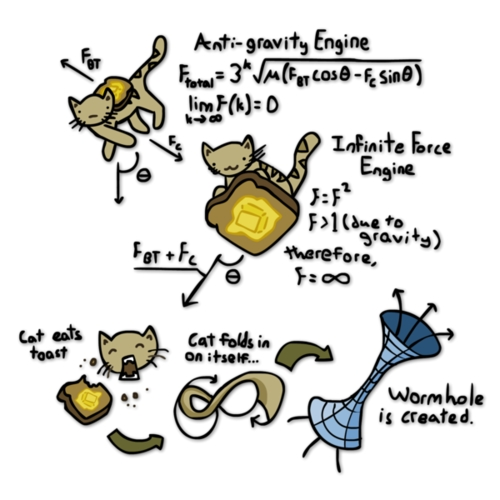
\includegraphics[height=.63\textheight]{bilder/Katze_Toast.jpg}
\end{center}

\von{Daniela, Marco und Ole}


\section{Anerkannte Beweismethoden der Lehrkörper}
\label{sec:beweise}
Extra für euch haben wir nun hier die wichtigsten Beweismethoden zusammengestellt:\\
\begin{description}
    \item[METHODE DER EXAKTEN BEZEICHNUNGEN:] Sei P ein Punkt Q, den wir R nennen.

    \item[AUTORITÄTSGLÄUBIGE METHODE:] Das muss stimmen. Das steht so im Bronstein.

    \item[KAPITALISTISCHE METHODE:] Eine Gewinnmaximierung tritt ein, wenn wir gar nichts beweisen, dann verbrauchen wir nämlich am wenigsten Kreide.

    \item[KOMMUNISTISCHE METHODE:] Das beweisen wir jetzt gemeinsam. Jeder schreibt eine Zeile, und das Ergebnis ist Staatseigentum.

    \item [NUMERISCHE METHODE:] Grob gerundet stimmt's!

    \item [BEWEIS DURCH EINSCHÜCHTERUNG:] Das ist doch wohl trivial!

    \item [BEWEIS DURCH ÜBERLADENE NOTATION:] Am besten verwendet man mindestens vier Alphabete und viele Sonderzeichen. Hier reicht das griechische Alphabet alleine nicht mehr aus, um engagierte Zuhörer abzuschrecken. Ein kurzer Exkurs in die hebräischen Sonderzeichen sollte aber auch den stärksten Zweifler zum Schweigen bringen.

    \item [BEWEISE DURCH AUSLASSEN:] 1. Die Details bleiben als leichte Übungsaufgabe dem geneigten Leser überlassen. 2. Die anderen 253 Fälle folgen völlig analog hierzu.

    \item [BEWEIS DURCH REDUKTION AUF DAS FALSCHE PROBLEM:] Um zu zeigen, dass dies eine Abbildung in die Menge der s-saturierten Ideale ist, reduzieren wir es auf die Riemannsche Vermutung.

    \item [BEWEIS DURCH REKURSIVEN QUERVERWEIS:] In Quelle a wird Satz 5 gefolgert aus Satz 3 der Quelle b, welcher seinerseits sofort aus Korollar 6.2 der Quelle c folgt, den man trivial aus Satz 5 der Quelle a erhält.

    \item [BEWEIS DURCH SCHEINVERWEIS:] Nichts dem zitierten Satz auch nur entfernt ähnliches erscheint in der angegebenen Quelle.

    \item [3-W-METHODE:] Wer will's wissen?

    \item [BEWEIS DURCH PAUSE:] Prof kurz vor der Pause: Diesen Satz beweise ich Ihnen nach der Pause. Prof nach der Pause: Wie wir vor der Pause bewiesen haben...
\end{description}
\section{Mentorenprogramm}
\textbf{Liebe StudienanfängerInnen,}
\medskip
herzlich willkommen am Fachbereich Physik!\\
Von der Schule kommend, ist vieles neu für Sie, manches an der Universität erscheint Ihnen vielleicht zunächst schwer zu durchschauen. Als eine Einstiegshilfe, die Ihnen über unnötige Klippen und Probleme am Anfang hinweghelfen soll, hat der Fachbereich seit einigen Jahren das bewährte Mentorenprogramm eingeführt; Ihnen wird ein/e Hochschullehrer/in zugeteilt, der oder die Ihr persönliche/r Mentor/in ist. Er ist Ihr direkter Ansprechpartner, der Ihnen für die ersten Semester zur Seite stehen soll. In einem persönlichen Gespräch lassen sich viele Schwierigkeiten des Anfangs oft viel besser als in Informationsveranstaltungen lösen.\\
Unser Fachbereich, Studierende und Lehrende, ist sehr familiär. Ihr Mentor ist eine Ihrer Kontaktstellen, um die Aufnahme in diesen Kreis zu erleichtern. Ihr Mentor soll nicht nur bei organisatorischen Problemen helfen, sondern Ihnen auch bei anderen möglichen Problemen mit dem Studium beistehen. Warum haben Sie sich für Ihr Physikstudium entschieden? Sprechen Sie mit Ihrem Mentor darüber, er kann Ihnen helfen, Ihre eigenen Ziele sicherer zu erreichen. Auch wenn er Ihnen nicht direkt helfen kann, wird er oft doch Kontakte vermitteln können. Sie haben Probleme mit der Finanzierung des Studiums? Vielleicht kann Ihnen Ihr Mentor eine Stiftung oder ein Stipendium empfehlen. Sie wollen ins Ausland? Ihr Mentor kann Ihnen viele Tipps geben. Sie fühlen sich vom Studium überfordert und wollen schon nach 2 Monaten alles hinschmei\ss en? Sprechen Sie mit Ihrem Mentor darüber, er kann Ihnen helfen, selbstkritisch zu prüfen, ob Physik das Richtige für Sie ist. Sie haben Ideen, was man am Studium verbessern könnte? Wo klemmt es am meisten? Ihr Mentor wird helfen, dass Ihre Anregungen aufgenommen werden.\\
Die Qualität des Studienangebotes lebt auch von Ihrem kritischen Feedback. Hier hat auch Ihr Studiendekan (zur Zeit der Autor dieses Textes) immer ein offenes Ohr.\\
Da der Fachbereich aus Gründen des Datenschutzes Ihre Kontaktdaten nicht hat, bitten wir Sie, sich bei der Einführungsveranstaltung auf die dort ausgelegte Liste für das Mentorenprogramm einzutragen. Geben Sie Ihre Adresse, Telefonnumer und E-Mail an. Ihre Adressen werden dann zufällig auf die Hochschullehrer verteilt. In den kommenden 3 Wochen sollten Sie dann eine Einladung zu einem Gespräch bekommen. Nehmen Sie die Gelegenheit wahr, lernen Sie gleich einen der Hochschullehrer etwas näher kennen und stellen Sie alle Fragen, die auftauchen, diskutieren Sie die Probleme, die Sie am Anfang haben.\\
Falls Sie innerhalb von 3 Wochen keine Einladung erhalten haben oder es verpasst haben, sich auf die Liste einzutragen, melden Sie sich bitte beim Dekanat des Fachbereiches Physik (798 47205, dekanat@physik.uni-frankfurt.de).\\
Einen guten Start in Ihr Physikstudium wünscht:\\
\von{
Prof. Dr. Joachim Maruhn\\
ehemaliger Studiendekan Fachbereich Physik
}
\section{Experimentelle Physik}

\begin{tabular}{p{0.2\linewidth}p{0.79\linewidth}}
  \textbf{Was:} & Mechanik und Thermodynamik\\
  \textbf{Wer:} & Prof. Dr. Ren\'e Reifarth, Dr. Kathrin Göbel\\
  \textbf{Wann/Wo:} & Mo: 11:00--13:00, Do: 10:00--12:00, Fr: 13:00-14:00, OSZ H1\\
\end{tabular}\\
\rule{\textwidth}{0.1pt}
\bigskip 

Das Vorlesungsprogramm zur experimentellen Physik wird mit dieser zweigeteilten Vorlesung zur Mechanik (bis Weihnachten) und zur Thermodynamik eröffnet.
In den darauf folgenden Semestern schließen sich dann Vorlesungen zur Elektrodynamik, zur Optik sowie zu den Themen "`Atome und Quanten"', "`Kerne und Elementarteilchen"' und "`Festkörper"' an.
Innerhalb der ersten vier Semester wird so in den Pflichtmodulen \Modul{VEX1A/B} bis \Modul{VEX4A/B} ein Überblick über die grundlegenden Erkenntnisse der Physik gegeben.
Zusätzlich werden Sie schon in den ersten Semestern auch viele Fragestellungen der aktuellen Physik kennenlernen.

Gerade zu Beginn des Studiums, in den ersten Vorlesungen, ist es wichtig, die Modell- und Begriffsbildung in der Physik anhand von Beispielen sorgfältig zu lernen und damit das Rüstzeug für ein tieferes Eindringen in die Physik zu erwerben.  

Zu Anfang der Vorlesung werden Ihr unterschiedlicher Wissensstand und Ihre unterschiedlichen Voraussetzungen aus der Schule noch eine Rolle spielen.
Die Vorlesung wird das berücksichtigen und wesentlichen Begriffe und Konzepte grundlegend behandeln.
Mit zahlreichen Experimenten in der Vorlesung sollen die Zusammenhänge noch besser veranschaulicht werden.
 
Besonders wichtig sind die die Vorlesung begleitenden Übungsaufgaben und Übungsgruppen (Tutorien).
Diese kleineren Übungs- und Lerngruppen finden einmal die Woche statt.
In der Vorlesung werden wöchentlich Übungsaufgaben ausgegeben, die Sie allein oder in Zweierteams bearbeiten sollen.
Die Lösungen der Aufgaben werden dann in den zweistündigen Tutorien besprochen.
So können Sie den Vorlesungsstoff am besten vertiefen. 

Für die Übungen melden Sie sich über das Webportal https://olat.server.uni-frankfurt.de an (siehe unten). Das Webportal ist
ab Donnerstag, 19.10.2017, 20:00 Uhr freigeschaltet.
Sie können zwischen verschiedenen Terminen wählen.
Eine Vorbesprechung zu den Übungen werden wir in der ersten Vorlesungsstunde durchführen.

Nach dem Ende der Vorlesungszeit finden zwei jeweils einstündige Klausuren statt. 
Die Termine werden in der Vorlesung bekannt gegeben.
Die erste Klausur (zur Mechanik) muss nur bestanden werden, sie bleibt unbenotet. 
Die Klausur zur Thermodynamik wird dagegen auch benotet.
Auch zu allen weiteren Vorlesungen des Zyklus finden benotete Modulabschlussprüfungen statt.
Zur Ermittlung der Bachelorgesamtnote am Ende des Bachelorstudiums kann allerdings eine Note aus der Wertung gestrichen werden.

Zu Beginn des Studiums wird nun vieles neu für Sie sein.
Lassen Sie sich von den formalen Regeln und Anforderungen eines Studiums, den Übungsaufgaben, Punkten, Klausuren und Prüfungen Ihren Spaß an der Physik nicht trüben.
Versuchen Sie immer das Studiensystem als angeleitetes Lernen zu sehen, damit Sie in möglichst kurzer Zeit mit den Begriffen und Methoden vertraut werden und das notwendige Werkzeug erwerben.

Nehmen Sie sich bei der Jagd nach den "`Credit-Points"' Zeit, um Ihre eigenen physikalischen Fragen und Ideen zu finden, versuchen Sie die Konzepte und Methoden wirklich zu verstehen und nicht nur für eine Klausur oder Prüfung zu lernen.
So sammeln Sie persönliches Wissen, Kenntnisse und Fertigkeiten. 

Einen guten Start für Ihr Studium.
\smallskip

\noindent
\textbf{Unterlagen zur Vorlesung}

\medskip
Der Stoff der Vorlesung wird an der Tafel entwickelt und mit Folienprojektion unterstützt.
Eine Mitschrift während der Vorlesung wird empfohlen.
Im Verlauf der  wird ein Skript zur Vorlesung angeboten
Eine kurze Einführung in "`Physik Online"'  wird in der Vorlesung gegeben.
Zur Vorlesung gibt es verschiedene Lehrbücher, die didaktisch hervorragend in das Thema einführen.
Parallel zur Vorlesung wird eine begleitende Lektüre sehr empfohlen.

Lehrbuchempfehlungen in alphabetischer Reihenfolge:

\noindent
\textbf{Literatur:}
\begin{itemize}
  \item Bergmann Schäfer, Band 1, Mechanik, Relativität, Wärme, Walter de Gruyter
  \item Demtröder, Experimentalphysik 1, Mechanik und Wärme, Springer Verlag
  \item Dransfeld, Kienle, Kalvius, Physik 1, Mechanik und Wärme, Oldenbourg Verlag
  \item Giancoli, Physik, einbändig, Pearson Studium
  \item Herrmann, Skripten zur Vorlesung Experimentalphysik - Mechanik, online
  \item Meschede, Gerthsen, Physik, einbändig, Springer Verlag
  \item Recknagel, Physik, Band 1, Mechanik, Verlag Technik Berlin
  \item Recknagel, Physik, Band 2, Schwingungen und Wellen, Wärmelehre, Verlag Technik Berlin
  \item Stöcker, Taschenbuch der Physik, Verlag Harri Deutsch   
  \item Tipler, Mosca, Physik für Wissenschaftler und Ingenieure, einbändig, Spektrum Verlag
\end{itemize}

Die Universitätsbibliothek hält einige Titel in großer Anzahl zur Ausleihe zu Verfügung, so dass Sie das/die für Sie passendste/n Buch/Bücher kostengünstig finden und nutzen können.
\noindent
\textbf{Anmeldung zur Übung:}

Sie können sich zu den Übungen auf dem OLAT System des HRZ anmelden.
Nach dem Einloggen in OLAT mit HRZ-Benutzername und Passwort klicken Sie unter "`OLAT-Schnellstart-Links"' auf "`Katalog"' und folgen dem Pfad:\\
$\hookrightarrow$ Lehrveranstaltungen des Fachbereichs 13 - Physik\\
$\hookrightarrow$ Bachelor- /Master-Studiengang "Physik"\\
$\hookrightarrow$ Bachelor-Studium "Physik"\\
$\hookrightarrow$ Pflichtveranstaltungen.\\
$\hookrightarrow$ Dann auf "`Übung zur Experimentalphysik 1"' klicken und für eine Übungsgruppe einschreiben.

\von{Prof. Dr. Ren\'e Reifarth}


\section{Anfängerfehler}

\begin{figure}[!b]
 \begin{center}
  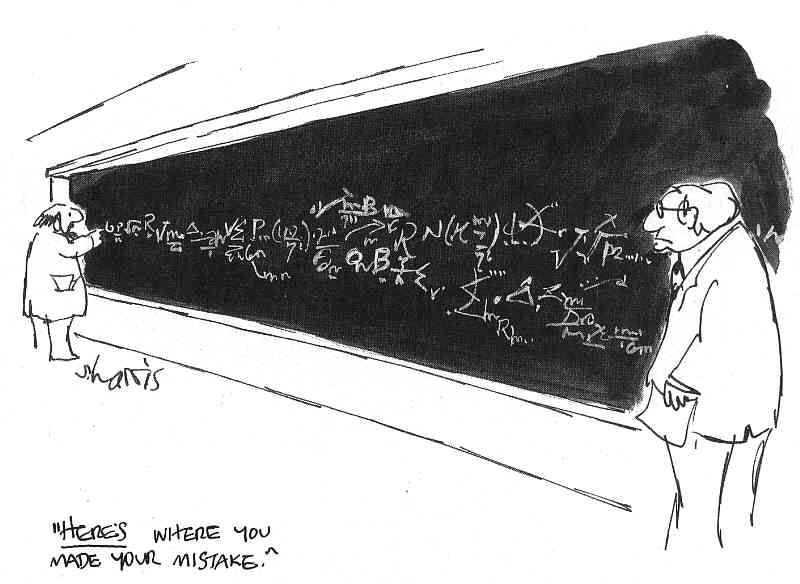
\includegraphics[height=6.5 cm]{bilder/mistake.jpg}
 \end{center}
\end{figure}

Das Wichtigste in der Anfängerzeit ist eigentlich: "`Büffeln, büffeln und noch mal büffeln``.\\
Besonders in Mathe und Theo--Physik werdet ihr bald zu der
Erkenntnis kommen, dass das, was die Professoren oft als so
"`trivial`` bezeichnen, in den Übungszetteln doch nicht so einfach ist.
Man kann natürlich die Zettel beim jeweiligen Matheass abschreiben.
Aber leider hat das keinen Sinn, da ihr den Stoff spätestens in der nächsten Modulprüfung brauchen werdet.\\
Und wie immer gilt auch hier die Regel:\\
"`\textbf{Ein selbst gemachter Fehler ist besser als eine abgeschriebene Musterlösung}.``\\
Naja, so viel dazu.
%
Ein anderer Punkt sind die Tutorien.
Es kann passieren, dass ihr euch einen Tutor aussucht, der vielleicht ganz
nett aussieht (und es höchst wahrscheinlich auch ist), dessen Stil
euch aber ganz und gar nicht liegt, weil er vielleicht die
Vektorpfeile unter die Variablen setzt oder so.
Vielleicht macht ihr ja ein Doppelstudium und zur Zeit eures Theoretikums habt ihr gerade
eine Vorlesung über Morphologie und Syntax afrikanischer Sprachen.\\
Das ist aber kein Problem, da ihr die Tutorien einfach wechseln könnt.
Besonders einfach geht das in der theoretischen Physik, da es dort unzählige Theoretika gibt.\\
%
Die wichtigste Regel lautet aber: "`Lernt in Gruppen!{}``.
Am meisten kann man lernen, wenn man die Themen der Vorlesung und die Übungszettel durchdiskutiert.
Des Weiteren findet man in einer Gruppe immer einen, der ein ganz bestimmtes Problem kennt.\\
Fragt! Fragt!! Und nochmals: Fragt!!!
Fragt Leute aus eurem Semester, fragt Leute aus den höheren Semestern und fragt die Professoren.
Gerade Professoren sind meistens begeistert über gute Fragen und stehen nach der Vorlesung
meistens sowieso noch an der Tafel herum.\\
%
Zu guter Letzt ist noch zu sagen: Lasst euch nicht hängen und gebt nicht auf.
Denn manchmal muss man sich ein bisschen anstrengen, um über den Berg zu kommen!

\von{Fritz}

% in dieser Datei werden weitere Dateien für jedes Nebenfach aus dem nebenfach Unterordner eingeladen
\section{Nebenfächer}
\label{sec:nebenfach}
Für den physikalischen Part eures Studiums wär`s das jetzt erst mal. Euer Stundenplan sieht jetzt schon relativ voll aus, ist aber noch nicht ganz fertig. Zu euren physikalischen Fächern kommen nämlich noch die Nebenfächer hinzu.\\
Als Nebenfach ist prinzipiell jedes nicht--physikalische Fach zugelassen. Ihr könnt auch zwei Nebenfächer studieren, wobei ihr beachten müsst, dass ihr am Ende eures Studiums mindestens 16--22 Credit~Points nachweisen müsst. Eigentlich sind hier der Phantasie der Wahl keine Grenzen gesetzt, die folgenden Fächer haben sich jedoch als \enquote{Standards} etabliert\ldots{}\\
Für eine Menge Nebenfächer sind Studienpläne vorgesehen, an die ihr euch halten müsst. Diese könnt ihr im Prüfungsamt einsehen. Wenn ihr jedoch viel lieber ein anderes Nebenfach belegen wollt, wie etwa \enquote{Zoologie der ost-usbekischen Steppe}, dann scheut euch nicht, bei Professor Maruhn nachzufragen, ob es möglich ist, dieses zu belegen.\\
Ein kleiner Tipp zum Nebenfach ist, dass ihr es möglichst früh belegen solltet, damit ihr immer noch Zeit habt, es zu wechseln. Oder stellt euch vor, dass ihr Stochastik als Nebenfach gewählt habt und dann nach einem Monat bemerkt, dass die Wahrscheinlichkeit, dass ihr dieses Nebenfach bis zum Ende bringen werdet, gegen Null geht\ldots{} Außerdem beginnen die meisten Nebenfächer nur im Wintersemester, einige auch nur im Sommersemester. Informiert euch also rechtzeitig.
\von{Fritz}
\begin{figure}
	\centering
	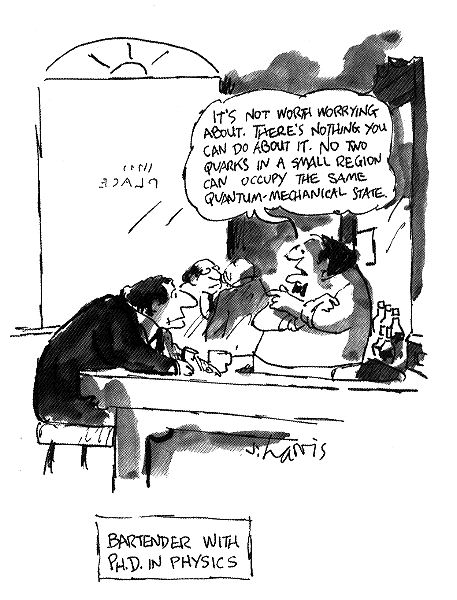
\includegraphics[width=0.4\textwidth]{\imgdir/bartender.jpg}
\end{figure}
\newpage
\subsection{Geophysik}
\label{subsec:geophysik}
Als Newton der Apfel auf den Kopf gefallen ist, kam ihm die Idee mit der Schwerkraft. Aber ist die wirklich überall gleich?Und als die Mauern von Troja zusammenstürzten, war das wirklich Poseidon? Und wieso dreht sich die Kompassnadel immer nach Norden? Oder tut sie das gar nicht?\\
All diese Fragen bekommst Du in der Physik, wenn überhaupt, nur am Rande erklärt, weil diese Sachen in den Bereich der \fach{Geophysik} gehören. Die Geophysik beschreibt unseren Planeten mit physikalischen Methoden. Dazu ist die Geophysik in verschiedene Unterbereiche eingeteilt, die sich nur mit einzelnen Teilen beschäftigen, dazu gehören die Bereiche Seismologie, Magnetismus, Schwerebeschleunigung und viele andere.\\
Aber warum soll ich jetzt Geophysik als Nebenfach machen? Und was kann ich damit anfangen? Naja, wenn Dich zum einen unser Planet interessiert, dann bietet es sich an, ein bisschen mehr darüber zu erfahren. Und wenn Du später in der freien Wirtschaft arbeiten willst, hast du mit Geophysik gute Chancen. Mit der Angewandten Geophysik kannst Du zum Beispiel Bodenschätze suchen und finden oder den Untergrund für Hochhäuser erforschen.\\
\begin{figure}[!h]
 	\centering
  	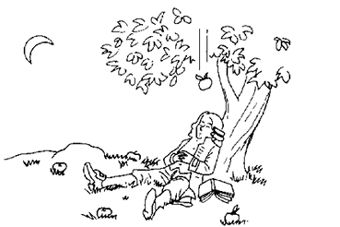
\includegraphics[width=.6\textwidth]{\imgdir/newton.jpg}
\end{figure}
Im ersten Modul Geophysik A (\Modul{GPA}), das Voraussetzung für die anderen beiden ist, erhälst Du mit der Vorlesung \VL{Einführung in die Geophysik} vorab einen Überblick über die Themen. Zu dieser Vorlesung gehört eine Übung, die Ihr besuchen müsst. Dazu kommen noch zwei weitere Vorlesungen, in denen Du Dich in einzelnen Bereichen spezialisierst. Eine der beiden Vorlesungen muss eine Übung haben. Abgeschlossen und benotet wird das Modul mit einer schriftlichen oder mündlichen Prüfung. Für dieses Modul erhälst Du 10 CP.\\
Das zweite Modul Geophysik B (\Modul{GPB}) setzt sich aus drei weiterführenden Vorlesungen zusammen, welche Du Dir ebenso wie die weiteren Vorlesungen im Modul \Modul{GPA} aussuchen kannst. Dadurch erhälst Du einen tieferen Einblick in die einzelnen Bereiche. Zu einer dieser Vorlesungen müsst Ihr an einer Übung teilnehmen. Ein Seminar, in dem Ihr selbst ein Thema auswertet und präsentiert, vervollständigt das Modul. Meistens wird das übergeordnete Thema vorgegeben und Du kannst dann aus einer Reihe von Themen wählen. Dabei betreut Dich einer der Professoren. Abgeschlossen und benotet wird das Modul wieder durch eine mündliche oder schriftliche Prüfung und Du erhälst auch hierfür 10 CP.\\
Als drittes Modul Geophysik C (\Modul{GPC}) gibt es ein Praktikumsmodul, bei dem Du richtige Messungen machst. Dabei kannst Du zwischen einem Laborpraktikum oder einem Feldpraktikum wählen. Bei dem Laborpraktikum machst Du verschiedene Versuche während des Semesters. Zu einem Versuch musst Du ein ausführliches Protokoll schreiben. Dieses Protokoll wird dann kontrolliert und ist der Abschluss dieses Moduls. Entscheidest Du Dich für das Feldpraktikum, fährst über vier Tage ins Gelände, machst Messungen und wertest diese anschlie\ss end aus. Die vier Versuche werden unter Anleitung eines Professors in Gruppen von ca 10 Studierenden gemacht. Zu einem ausführlichen Protokoll, das Abschluss des Moduls ist, musst Du eine weitere Vorlesung aus dem Bereich der Angewandten Geophysik hören. Das Feldpraktikum ist zwar somit mehr Aufwand, lohnt sich aber auf jeden Fall. Für dieses Modul erhälst Du nach dem erfolgreichen Protokoll unbenotet 5 CP.\\
Geophysik ist also die Physik richtig Anwenden und macht eine Menge Spa\ss . Solltest Du Dich für Geophysik als Nebenfach entscheiden, hast Du sicher keine falsche Wahl getroffen.
\von{bur}
\subsection{Astrophysik}
\label{subsec:astro}
Es ist ein warmer Sommerabend und du bist mit deinen Freunden am Strand oder in einem Park unterwegs und ihr schaut euch die Sterne an. Während alle anderen nur das romantische Bild des Himmels genie\ss en, überlegst du dir, wie weit der Stern ganz im Süden wohl ist, ob es überhaut ein Stern oder doch ein Plantet ist, was in seinem Inneren vorgeht? Wenn dir diese Situation bekannt vorkommt, ist \fach{Astronomie} als Nebenfach das Richtige für dich. Hier lernt man, das Universum physikalisch zu verstehen. Das bedeutet, es ist kein Nebenfach für reine Sterngucker, die möglichst viele hübsche bunte Bilder sehen wollen (keine Angst, die gibt es aber natürlich auch), sondern man beschäftigt sich mit Strahlungsprozessen, den Geschehnissen in unserer Sonne und unserem Planetensystem. Gerade das Kapitel Strahlung wirkt zu Beginn leicht abschreckend, stellt aber nach anfänglichen Schwierigkeiten kein grö\ss eres Problem dar.\\
Mit \fach{Astronomie} als Nebenfach könnt ihr bis zu 25 CP's sammeln und damit sogar die 22 CP, die ihr maximal für den Bachelor braucht, abdecken. Dabei ist es in zwei Module aufgeteilt: Das erste Modul, welches euch 12 CP gibt, besteht aus zwei Vorlesungen, die ihr ohne Probleme in den ersten beiden Semestern hören könnt. Dort werdet ihr euch vor allem mit der Sternentwicklung, Planetensystemen, unserer Sonne und Galaxien beschäftigen. Im zweiten Modul müsst ihr eine Spezialvorlesung hören und an einem Praktikum sowie einem Seminar teilnehmen. Im Allgemeinen kann man das Praktikum, welches nur im Sommersemester angeboten wird, schon im 2. Semester machen, da die einzige Voraussetzung die \VL{Astro1} Vorlesung ist. Somit könnt ihr mit eurem Nebenfach nach dem 3. Semester fertig sein, was insofern ganz praktisch ist, da man in den höheren Semestern noch Wahlpflichtveranstaltungen belegen muss, wofür man so mehr Zeit hat. Au\ss erdem ist der Praktikumsinhalt auf die 2. Vorlesung abgestimmt, ihr könnt damit also sehr leicht euer Wissen verfestigen. Zum Ende des 2. Semesters kommen nun endlich auch die Sternegucker unter euch auf ihre Kosten. Im Rahmen des Praktikums wird eine Beobachtungsnacht auf dem kleinen Feldberg veranstaltet, bei der ihr viele der von euch zuvor theoretisch untersuchten Objekte auch mal live sehen könnt. Für das Modul \Modul{AstroB} erhaltet ihr 13CP's.
%Gehalten werden alle Vorlesungen und das Praktikum von Professor T. Boller, der eigentlich am MPE, dem Max-Planck-Institut für extraterrestrische Physik in Garching bei München, arbeitet und jeweils einmal pro Woche an die Universität Frankfurt kommt.
%Dies weist den Vorteil auf, dass er an aktuellster Forschung beteiligt ist, was in der Vorlesung seinen Einfluss findet.
\von{Patricia}
\begin{figure}[!t]
 	\centering
  	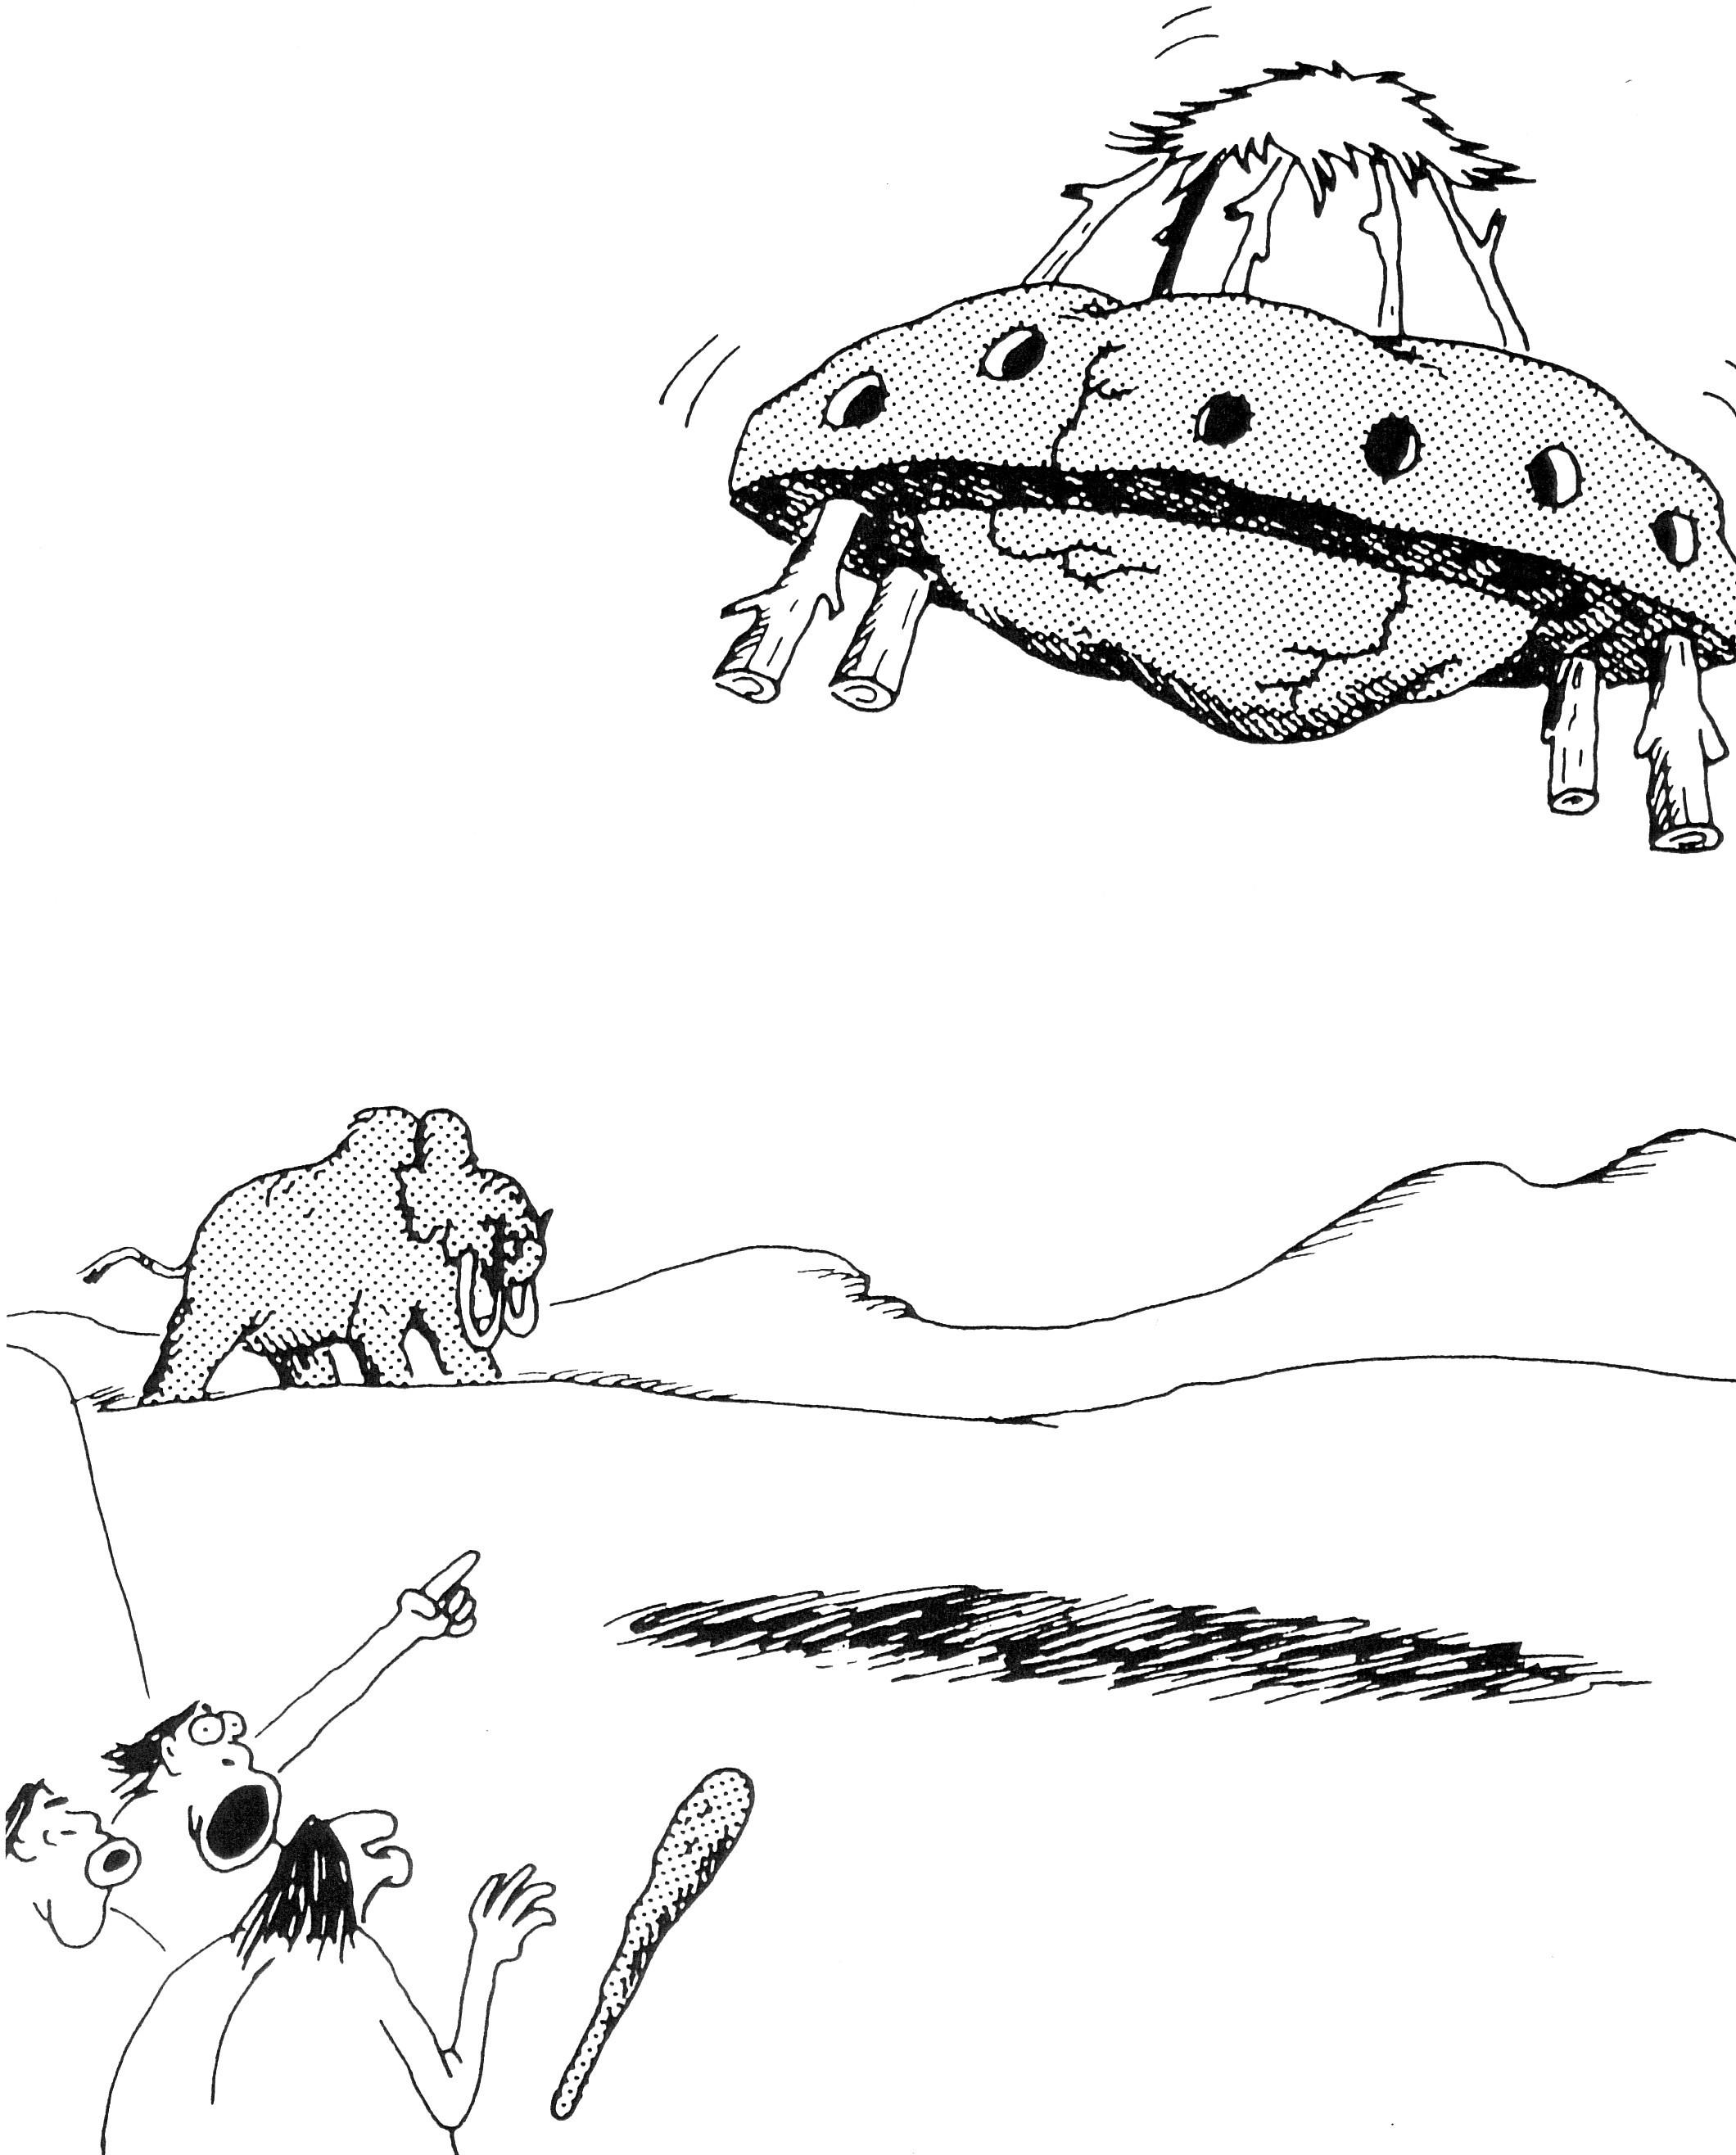
\includegraphics[width=.4\textwidth]{\imgdir/steinufo.jpg}
\end{figure}
\subsection{Meteorologie}

Ich persönlich studiere Meteorologie auf Diplom und Physik auf Bachelor, habe daher selber Meteorologie als Nebenfach belegt. 
Im Folgenden möchte ich euch dieses Fach als Nebenfach vorstellen.\\
\fach{Meteorologie} ist ein sehr interessantes Fach, da es ziemlich viel mit Physik zu tun hat, das Thema aber einmal von einer anderen Perspektive angeht.
Es handelt sich dabei um eine noch sehr wenig erforschte Wissenschaft, die man aber im alltäglichen Leben leichter beobachten kann als einige andere Nebenfächer, die an der
Uni Frankfurt angeboten werden.\\
Nun aber zu den Inhalten und den Dingen, die ihr für dieses Fach leisten müsst.\\
Laut Bachelor - Prüfungsordnung können alle Module der bestehenden Bachelorordnung des Bachelorstudiengangs Meteorologie gewählt werden.\\
Ihr fangt mit dem Modul \Modul{EMet A} an.
Dieses umfasst die Vorlesungen \VL{Allgemeine Meteorologie} und \VL{Klimatologie} und gibt insgesamt 10 CP.\\
In der allgemeinen Meteorologie geht es z.B. um meteorologische Grundbegriffe, die Struktur der Atmosphäre und um Windgesetze. 
\begin{figure}[!t]
  \begin{center}
  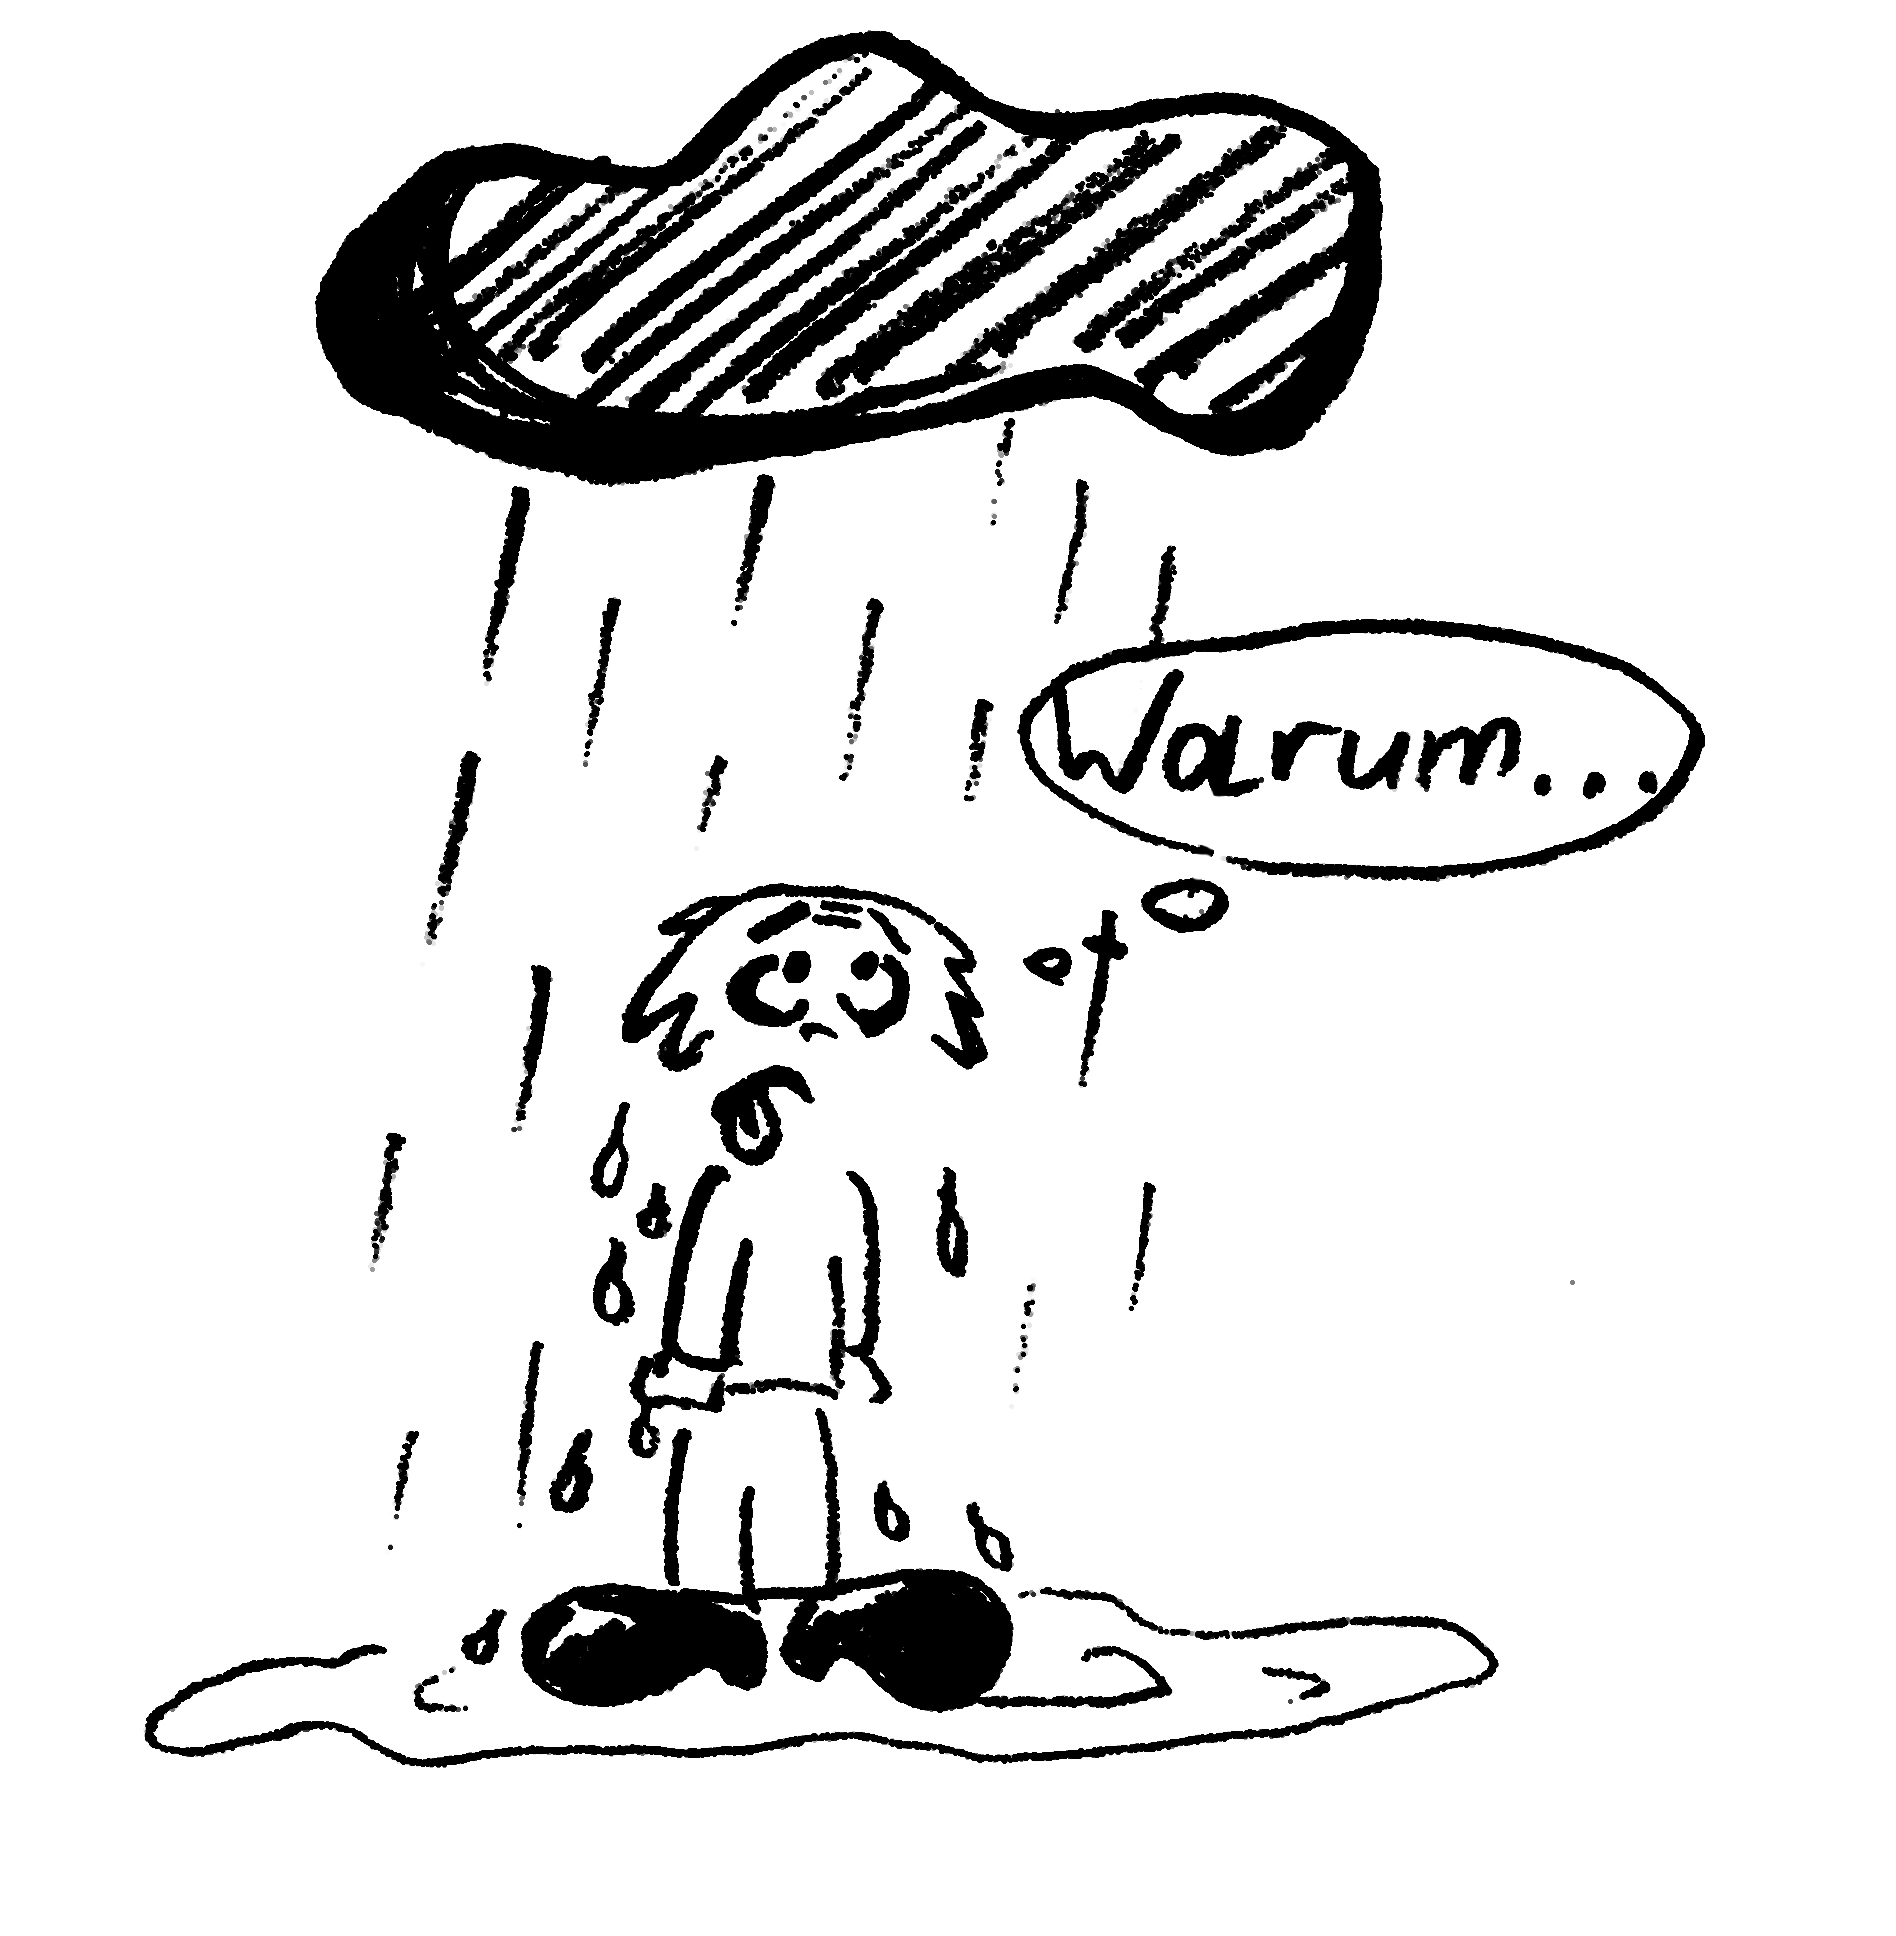
\includegraphics[width=.7\textwidth]{bilder/meteorologe.jpg}
\end{center}
\end{figure}

\pagebreak

Die Klimatologie betrachtet nicht kurzlebige Phänomene wie das Wetter, sondern lange Zeiträume von mindestens 30 Jahren.
Prof. Dr. Bodo Ahrens erklärt, wie man Klima "`macht"', also wie man es mit statistischen Methoden bestimmt und welche meteorologischen Größen dabei eine Rolle spielen.
\bigskip

Danach könnt ihr mit dem Modul \Modul{EMet B} weitermachen.
Dafür bekommt ihr auch 10 CP.
\\Das Modul umfasst eine Einführung in die Theoretische Meteorologie (\VL{Atmospheric Dynamics I} und \VL{II}).
\\Die Theoretische Meteorologie beschäftigt sich unter anderem mit der Kinematik des Windfeldes, der Newtonschen Mechanik und mit Thermodynamik.
\bigskip

Mit dem Modul \Modul{EMet A} könnt ihr direkt im Wintersemester anfangen.
Es sind keine Vorkenntnisse notwendig.
\von{Luisa}

\subsection{Informatik}
%Im Unterschied zur Physik, die beschreibt "`was ist``, versucht die Informatik, Handlungsanweisungen und Konzepte zu geben, um grosse Datenmengen (Informationen) effizient verarbeiten zu können. Dazu werden in der Vorlesung grundlegende Konzepte für Handlungsanweisungen (Algorithmen), ihre sprachliche Formulierung (Programme) und ihre Informationen (Daten) vorgestellt und gelernt. Dies dient dazu, Struktur und Design sowie den Einsatzbereich verschiedener Programmiersprachen zu erkennen und einschätzen zu können, um für ein gegebenes Problem die geeignete programmtechnische Formulierung zu wählen. Aber auch den Lebenszyklus von Software und elementare Prozesse und Methoden der Software--Entwicklung lernen wir kennen. Weiterhin wird die Ablaufumgebung, also die typischen Konzepte und Eigenschaften von Betriebssystemen, erläutert, um bei Problemen konstruktiv eingreifen zu können. Dazu zählen beispielsweise die Problemfelder IT--Sicherheit und Netzwerke. Im zweiten Teil der Vorlesung werden die Programmiersprachenkonzepte von Syntax und Semantik um die Bereiche der funktionalen und objektorientierten Sprachen erweitert und damit das Verständnis von Programmiersprachen vertieft. Dazu kommt die Modellierung, Verwaltung und Nutzung großer Datenbestände mit Hilfe von Datenbanken.
%\von{Rüdiger Brause}


\fach{Informatik} ist ein durchaus nützliches Nebenfach, da das Programmieren oft ein wichtiges Hilfsmittel
für Physiker darstelllt. 
So vielseitig wie der Studiengang Informatik kann auch dieses Nebenfach werden, 
denn es lassen sich alle Module wählen und beliebig kombinieren. 
Will man das Fach einbringen, muss man jedoch die Vorlesung \VL{Grundlagen der Programmierung 1} (\Modul{PRG-1})
mit Übung belegen und die Klausur, die meist noch in der Vorlesungszeit geschrieben wird, bestehen.
Diese Vorlesung gibt einem einen guten und strukturierten Überblick über die Themengebiete der Informatik, 
sie ist aber gleichzeitig auch ein Schnupperkurs zur Programmierung.
Belohnt wird dies mit 11 CP.
Anschließend kann man, zum Beispiel im Sommersemester,
mit \VL{Datenstrukturen} oder \VL{Hardwarearchitekturen und Rechensysteme} weitermachen.
Das Nebenfach ist ab dem ersten Semester geeignet.
Da \Modul{PRG-1} nur im Wintersemester angeboten wird, ist es auch sinnvoll, damit gleich anzufangen.
\fach{Informatik} ist auf jeden Fall ein interessantes Nebenfach, sowohl für diejenigen mit Vorkenntnissen,
um diese zu strukturieren und zu vertiefen, als auch für diejenigen ohne Vorkenntnisse,
um einen Überblick über das Fachgebiet zu erhalten.
\von{Rita}

\begin{center}

  
\includegraphics[width=0.35\textwidth]{bilder/einstein.jpg}

\end{center}

\subsection{Geschichte der Naturwissenschaften}

Geschichte der Naturwissenschaften - was soll das den sein?
... Habe ich mir auch gedacht und bin einfach mal in der ersten Woche hingegangen.\\
Dieses Nebenfach besteht aus mehreren kleinen Seminaren mit jeweils zwei Stunden die Woche, ist also ziemlich gut neben den Pflichtvorlesungen zu machen.\\

Nun aber zum Inhalt:
In \fach{Geschichte der Naturwissenschaften} geht man der naturwissenschaftlichten Begriffs- und Theorienbildung auf den Grund.
Woher kommen zum Beispiel die Begriffe \textit{Kraft} und \textit{Energie}?
Wie hat sich unser Weltbild im Laufe der Jahrtausende langsam entwickelt?
Worin sind unsere heutigen Denkstrukturen begründet?
Wenn ihr diese Fragen interessant findet, ist \fach{Geschichte der Naturwissenschaften} wirklich sehr zu empfehlen.\\

Im Moment unterteilt sich das Fach noch in zwei Module, von denen eines 12 CP und eines 13 CP liefert:\\
Das 12 CP - Modul trägt den Titel \Modul{Einführung in die Naturphilosophie}.
Wie der Name schon sagt, beschäftigt man sich hier in drei eher philosophischen Seminaren mit den Anfängen wissenschaftlichen Denkens.
Haupsächlich wird hier die Antike behandelt.\\
Das 13 CP - Modul heißt \Modul{Einführung in die Geschichte der Naturwissen- schaften}.
Auch dieses Modul teilt sich wieder in drei Seminare auf, deren Themen von Semester zu Semester variieren.
Relativ oft wird die klassische Mechanik im 17. und 18. Jahrhundert behandelt.
Ansonsten betrachtet man die Originaltexte einzelner Mathematiker und Physiker dieser Zeit.
Oft werden die Texte auch in der Original-Sprache vorgelegt, interessant, wenn man in der Schule Französich oder Latein gelernt hat.
Das ist allerdings keine Voraussetzung, es gibt auch immer Übersetzungen zumindest ins Englische.\\

Jedes Seminar ist benotet.
Wie die Note zustande kommt, hängt allerdings am Dozenten:
Es kann also ein Kurzvortrag sein oder auch eine Hausarbeit.\\

Das Nebenfach lässt sich in drei Semestern abschließen.
Alles in allem ist \fach{Geschichte der Naturwissenschaften} ein sehr angenehmes Nebenfach, das eine willkommene Abwechslung zum Pflichtbereich ist.

\von{Miriam}

\subsection{Elektronik}
\label{subsec:elektronik}
Das Nebenfach \fach{Elektronik} besteht aus zwei Modulen, die beide belegt werden müssen. Mit beiden kann man innerhalb von zwei Semestern 16 Credit Points bekommen.\\
Das Nebenfach fängt immer im Wintersemester an mit \Modul{Elek1}.
Darin enthalten sind zwei Vorlesungen. \VL{Elektronik und Sensorik} (2 SWS + 1 SWS Übung) im Wintersemester und im darauffolgenden Sommersemester die Vorlesung \VL{Digitalelektronik} (2 SWS). Parallel dazu läuft im Sommersemester ein Praktikum, das Modul \Modul{Elek2}. Das ist wiederum in einen Digital- und einen Analogteil aufgeteilt. Die Credit Points gibt es, wenn man alle Protokolle mit OK zurück hat und eine mündliche Prüfung zu den Vorlesungen hinter sich hat, wobei diese Note als Note für das komplette Nebenfach zählt. In Elektronik ist man meist in einer recht überschaubaren Gruppe, was eine gute Lernatmosphäre schafft.\\
Zu den Themen:\\
Die Analogelektronik beschäftigt sich erst mal mit den grundlegenden elektronischen Bauteilen, wie Widerstand, Spule, Kondensator und den hieraus bestehenden Schaltungen (sogenannte lineare passive Netzwerke). Danach kommen die Halbleiterbauelemente wie Dioden, Bipolartransistoren und Feldeffektransistoren etc dran, sowie eine Einführung in die Sensorik.\\
In der Digitalelektronik werden diese Bauteile dann genutzt um logische Schaltungen aufzubauen, welche mit Boolscher Algebra beschrieben werden können. Au\ss erdem werden Zustandsautomaten, Speicher und Mikroprozessoren besprochen. Hier erhält man sehr interessante Einblicke in das Innenleben von Computern.\\
Allerdings kommt man um einiges an Mathematik nicht drum herum. Deswegen hat man auf jeden Fall einen Vorteil, wenn man schon ein Semester hinter sich hat und zumindest die Grundlagen der Elektrodynamik und Fourier-Analyse kennt. Wen es aber wirklich interessiert, für den sind sicher auch mangelnde Vorkenntnisse kein Problem! Also, einfach mal ausprobieren.
\von{Berit und Martin}
\subsection{Philosophie}
\label{subsec:philosophie}
\textit{\enquote{Ich wei\ss , dass ich nichts wei\ss !}}\\
Das wissen eigentlich alle oder? Warum also noch Philosophie studieren?\ldots Warum eigentlich \"uberhaupt irgendetwas machen? Warum handeln Menschen oder erst einmal: Gibt es uns Menschen denn? und wenn ja, was gibt es noch?
\begin{figure}[!b]
  	\centering
	
\includegraphics[width=.275\textwidth]{\imgdir/Ich_weiss.jpg}
\end{figure}
Viele Fragen gibt es in der Philosophie, das ist wohl wahr\ldots Aber halb so wild, denn was ist schon \enquote{Wahrheit}?\\\\
W\"ahlst du \fach{Philosophie} als Nebenfach, wirst du dich mit all diesen Fragen besch\"aftigen m\"ussen. Du wirst \"uber die Metaphysik und die Erkenntnistheorie diskutieren und du wirst dir bez\"uglich so mach einer Meinung die Hand vor den Kopf schlagen oder erstaunt die Augen \"offnen.\\
Das Philosophiestudium ist eines der vielseitigsten und wenn du denken und diskutieren magst, auch eines der spa\ss igsten \"uberhaupt. Und als Erg\"anzung f\"ur die sonst so klinischen Physiker-Nerds ideal geeignet.\\
Das gilt \"ubrigens auch anders herum. Es ist erstaunlich, wie oft dir in der Philosophie die Physik begegnet. Mein Tutor zog die Quantenmechanik mindestens einmal pro Stunde als Beispiel heran =)\\
Das Philosophiestudium beginnst du mit einem der Basismodule (\Modul{BM}).
Im \Modul{BM1} hast du 2x2 SWS Vorlesung und ein 1x2 SWS Tutorium.
Die Vorlesung sieht folgenderma\ss en aus:\\
Jeder Student kauft sich eine Mappe mit philosophischen Texten (auch online verf\"ugbar), welche gelesen werden m\"ussen und nach und nach in den Vorlesungen besprochen werden. Im Tutorium sieht man sich den Text dann noch genauer an und merkt, wie wenig man ihn eigentlich verstanden hat :P\\
Abgeschlossen wird das Modul durch eine Klausur und bringt dir dann 12 CP.\\
Auch sehr interessant ist es als Physiker \Modul{Logik} zu h\"oren. Hier lernt man n\"amlich, wie man logisch richtige Argumente hervorbringt und was zum Beispiel logische Fehlschl\"usse sind.\\
Dazu kannst du eines der \Modul{AM} (Aufbaumodule) belegen, welche 8CP's bringen. Welche \Modul{AM's} angeboten werden, kannst du im aktuellen Vorlesungsverzeichnis nachlesen. Als Besonderheit ist zu beachten, dass du als Nebenf\"achler alle Aufbaumodule besuchen darfst, auch wenn sie als Vorraussetzung Vorlesungen haben, die du nicht geh\"ort hast.
\von{Marco}
\subsection{Chemie}

Das klassische Physiker-Nebenfach ist eindeutig \fach{Chemie}. Das ist nicht 
verwunderlich, da sich die Themen oft gut erg\"anzen. \fach{Chemie} geh\"ort 
außerdem zu den Nebenf\"achern mit den meisten Modulen, sodass man sich aus 
einer grossen Auswahl zusammenstellen kann, was einen am meisten interessiert.
Oder man kombiniert mit einem anderen Nebenfach. Auf jeden Fall muss man die
Vorlesung \VL{Allgeime und anorganische Chemie}
(Modul \Modul{ChemA}) sowie ein Praktikum (Modul \Modul{ChemB} oder \Modul{PCP}) besuchen. Alle 
weiteren Module sind danach optional.\\
Ein grosser Vorteil dieses Nebenfachs ist zweifellos auch, dass die 
Chemie-Geb\"aude \glqq nebenan\grqq ~sind, d.h. Campus-Pendeln entf\"allt.
\\
\\
1.Semester:\\
Vorlesung \VL{Allgeime und anorganische Chemie}
(Modul \Modul{ChemA}, 7CP). \\
In dieser Vorlesung geht es allgemein um die Grundlagen 
der Anorganischen und Physikalischen Chemie. Im Prinzip: Atome und Molek\"ule,
Thermodynamik, chemisches Gleichgewicht, S\"auren und Basen, Elektrochemie 
und nat\"urlich einmal quer durchs Periodensystem - eine Auffrischung der 
der kompletten Schulchemie und mehr.\\
Am Ende des Semesters wird eine Klausur geschrieben, nach deren Ausgang die 
Praktikumspl\"atze vergeben werden. Diese Klausur ist aber kein Hindernis -
in der Regel schneiden Physiker dabei ganz gut ab.\\
Die Vorlesung selber teilen sich zwei Professoren: Prof. Auner,
Prof. Martin Schmidt und Prof Buchsbaum. Gewechselt wird um Weihnachten herum. Der erste Teil 
ist eher etwas trocken, aber der zweite Abschnitt kompensiert das ganz gut.
Dann werden auch mal Experimente vorgef\"uhrt und Anschauungsmaterial
mitgebracht.\\
Wer also schon immermal Silizium-Wafer in der Hand haben wollte, oder die 
Kristalle der verschiedenen Elemente und Verbindungen sehen wollte, der ist 
hier gut aufgehoben. Einige interessante Themen sind: \\
Gewinnung von Aluminium und Silizium, warum Diamant nicht ewig h\"alt, 
Funktionsweise von Laserdruckern und Kopierern, Photographie, Halbleiter ...
um nur ein paar Dinge zu nennen.\\
\\
Nachteile will ich auch nicht verschweigen: Zumindest am Anfang ist der 
H\"orsaal ziemlich voll, da diese Vorlesung f\"ur andere Studieng\"ange 
Pflichtveranstaltung ist. Ausserdem liegt die Vorlesung f\"ur Langschl\"afer
und Weitgereiste ung\"unstig, n\"amlich gleich Montag und Mittwoch von 
8-10 Uhr.\\
Zu dieser Veranstaltung wird eine \"Ubung (Teilnahme freiwillig) angeboten.\\
\\
2.Semester:\\
Praktikum \VL{Chemie f\"ur Naturwissenschaftler} (\Modul{ChemB}, 3,5CP)\\
Das Praktikum ist vierst\"undig angesetzt, aber wenn man es gut organisiert, 
braucht man wesentlich weniger Zeit. Es geht dabei haupts\"achlich um
 anorganische Chemie und ihre Anwendungen, wie z.B. Titration, 
Nachweisreaktionen, pH-Wert-Bestimmung und Trennmethoden. Insgesamt sind es 
acht Versuchstage und jeweils ein Seminar dazu. Auch hier wird am Ende wieder 
eine Klausur geschrieben, deren Stoff aber wesentlich weniger umfangreich ist,
als im ersten Semester. Bei den Versuchstagen ist Kitteltragen durchaus 
sinnvoll, sonst hat man pl\"otzlich L\"ocher in der Kleidung, wo eigentlich 
keine sein sollten. Insgesamt macht es viel Spaß, die verschiedenen 
L\"osungen zusammenzumixen und man erlebt dabei immer wieder \"Uberraschungen.\\
Als Alternative kann das Praktikum \VL{Physikalische Chemie} besucht 
werden (\Modul{PCP}, 5,5CP).\\
\\
Hier noch eine kleine Auswahl weiterf\"uhrender Module:\\
\Modul{Physikalische Chemie I} (Therm, 6CP),\\
\Modul{Organische Chemie} (Org, 7CP),\\
\Modul{Festk\"orperchemie} (ChemF, 3CP).\\
\\
Chemie ist auf jeden Fall ein lohnendes und interessantes Nebenfach, wenn man 
ein bisschen panschen will und sich auch f\"ur andere Naturwissenschaften 
interessiert, denn Chemie verbindet im Prinzip Physik, Biologie und 
Geowissenschaften miteinander. Super. 
\von{Kristin}

\subsection{Nuklearmedizin}  %wie viele CP es n\"achstes mal geben wird muss erst noch gekl\"art werden
\label{subsec:nuklearmedizin}
\enquote{Oh mein Gott, wir brauchen Hilfe! Ist ein Arzt anwesend?}\\
Auf diese Frage wolltest du schon immer einmal mit \enquote{Ja!} oder \enquote{Aus dem Weg, ich bin Arzt!} antworten?\\
Hm, ich auch, aber da hilft dir dieses Nebenfach nicht wirklich weiter. Auch wenn der Name es suggestiert, \fach{Nuklearmedizin} macht dich nicht zum Mediziner. Du lernst zwar etwas \"uber die Grundlagen der menschlichen Anatomie (Leber, Schilddr\"use und Co), aber im Wesentlichen geht es um die physikalischen Eigenschaften von Radionukliden und ihre Anwendungsm\"oglichkeiten in der Medizin. Hierzu besch\"aftigst du dich z.B. mit folgenden Fragen:
\begin{itemize}
  \item{Warum strahlen manche Stoffe?}
  \item{Was ist Strahlung \"uberhaupt und welche Varianten gibt es?}
  \item{Welche Strahlung wirkt wie auf die Zellen und warum?}
  \item{Wie schaffe ich es, dass genau der Bereich verstrahlt wird, den ich bestrahlen will und sonst keiner?}
  \item{Wie nutze ich Strahlung zur Diagnostik? (Detektorphysik)}
  \item{Wie lese ich CT/MRT oder PET Bilder?}
\end{itemize}
Und vielen weiteren. Alles in allem stellt es eine gelungene Symbiose aus Medizin, Zellbiologie und Physik dar und hilft dir, \"uber den (sowieso schon gro\ss en, aber immer noch erweiterbaren) Physikerhorizont hinaus zu blicken.\\\\
Jetzt zu den Fakten:\\
Das Nebenfach muss \"uber 2 Semester belegt werden und umfasst pro Semester 4 SWS, die anwesenheitspflichtig sind. Dazu kommt in der vorlesungsfreien Zeit nach dem 2. Semester ein zweiw\"ochiges Praktikum in der Uniklinik oder im Klinikum Hanau, in dem du das Gelernte anwenden und vertiefen kannst.\\
Abgeschlossen wird \fach{Nuklearmedizin} mit einer m\"undlichen Pr\"ufung,
in der jeweils 15 min der medizinische und physikalische Bereich abgefragt werden. Von den 20CP können bis zu 6 CP als Wahlpflicht eingebracht werden.
\von{Jonas}
\bigskip
Das wars dann soweit von den Nebenfächern. Wenn es zu diesem Thema noch Fragen gibt, dann ist es am besten für euch, direkt bei den Dozenten oder den sogenannten \enquote{Modulbeauftragten} nachzufragen. Eine andere Methode ist es, beim Prüfungsamt nachzufragen.\\
Ihr könnt natürlich auch uns kontaktieren. Um den Tipp von vorhin nochmal zu wiederholen \ldots\\
Belegt am Anfang, d.h. in der ersten Woche mal alle Nebenfächer, die euch näher interessieren und sucht euch dann eins daraus aus!\\
Viel Spa\ss\space bei euren Nebenfächern.
\section*{Notizseiten}
\cleardoubleevenpage 
\section{Unistruktur}

\subsection{Einleitung}
Die Universität verwaltet sich selbst. Das bedeutet, sie muss selbst zusehen, wie sie mit den ihr zur Verfügung gestellten finanziellen Mitteln auskommt und entscheiden, was sie damit macht. Das ist gar nicht so einfach, schlie\ss lich haben nicht nur satte 16 Fachbereiche ihre eigenen Interessen, sondern auch zahlreiche weitere Einrichtungen, wie etwa die Bibliothek, wollen hier mitreden.

\subsection{Uniweites}
Um das alles unter einen Hut zu bekommen und die Universität nach au\ss en zu vertreten, gibt es eine Unileitung, das Präsidium, und einen Chef, den Präsidenten.\\
Weil der nicht alles alleine machen möchte, gibt es noch ganze 4 Vizepräsidenten (darunter auch eine Physikerin), einen Kanzler und jede Menge Ausschüsse. In diesen Gremien sind sämtliche Angehörige der Universität, also Professoren, Wissenschaftliche und Administrativ-Technische Mitarbeiter und natürlich auch wir, die Studierenden, vertreten. Allerdings ist das nur halb so demokratisch, wie es scheint, da die Professoren überall die absolute Mehrheit an Stimmen haben. Jedoch sind sie sich auch nur halb so einig, wie man vielleicht denken mag.\\
Die beiden wichtigsten Gremien sind:

\subsubsection{Der Senat}
Der Senat ist das wichtigste Gremium auf Uni--Ebene. Er entscheidet über die Entwicklung und die Forschungsschwerpunkte der Uni. Der Senat besteht aus 9 Professoren, 3 Studierenden, 3 Wissenschaftliche Mitarbeiter und 2 Admininistrativ-Technische Mitarbeiter.

\subsubsection{Der Hochschulrat}
Der Hochschulrat ist eine recht neue Erfindung. Der Hochschulrat übernimmt seit die Uni Frankfurt eine Stiftungsuni ist die Kontrollfunktion, die damals das Ministerium für Wissenschaft und Kunst des Landes Hessen innehatte. Dem Hochschulrat gehören elf externe Mitglieder aus den Bereichen Wissenschaft, Wirtschaft und Kunst an. Er hat das Initiativrecht zu grundsätzlichen Angelegenheiten der Hochschulentwicklung, benennt und entlastet den Präsidenten und bildet aus den eigenen Reihen (+ einem Vertreter aus dem Ministerium der Finanzen) einen Wirtschafts- und Finanzausschuss.

\subsection{Studierendenvertretung}
Darüber hinaus gibt es dann aber noch die studentische Selbstverwaltung, das ist das Studierendenparlament (StuPa) und der Allgemeine Studierendenausschuss (AStA).

\subsubsection{Das StuPa}
Hier sitzen ausschlie\ss lich Studierende. Da diese zur Gruppenbildung neigen, gibt es, ähnlich den Parteien und zum Teil mit diesen verbunden, verschiedene Listen, die die Mitglieder des StuPas stellen oder dies gerne würden.\\
Zur Zeit sind dies die Grüne Hochschulgruppe, Juso-Hochschulgruppe, Giraffen - Unabhängige Fachbereichsgruppen, RCDS - Ring Christlich-Demokratischer Studenten, Schildkröten, LHG - Liberale Hochschulgruppe, attac/independent students, Die Linke.SDS, Pinguine, LiLi - Wahlbündnis Linke Liste, DL - Demokratische Linke Liste, FDH - Fachschafteninitiative Demokratische Hochschule und noch einige mehr.\\
Glücklicherweise erhalten nicht alle dieser Gruppen ausreichend Stimmen, um Mitglieder ins StuPa entsenden zu können.

\subsubsection{Der AStA}
Der AStA ist so etwas wie die Regierung des StuPas. Er besteht aus sogenannten Referaten, die sich um die Belange der Studierenden zu unterschiedlichsten Themen kümmern. Für die Arbeit der Referate stehen dem AStA etwa 500.000 \euro{} pro Jahr zur Verfügung, zum Teil auch durch die studentischen Beiträge finanziert.

\subsection{In der Physik}
Auch der Fachbereich besitzt eine eigene Verwaltung, sein Chef ist der Dekan.

\subsubsection{Der Fachbereichsrat (FBR)}
Äquivalent zum Senat auf Uniebene entscheidet der FBR über die Belange des Fachbereichs Physik. Den Vorsitz hat der Dekan, der auch den gesamten Fachbereich nach au\ss en vertritt. Der Fachbereichsrat richtet für alles mögliche Ausschüsse ein, beispielsweise zur Erarbeitung der Studien-- und Prüfungsordnung.

\subsubsection{Der Fachschaftsrat (FSR)}
Alle Physikstudierenden gemeinsam sind die Fachschaft. Diese wählt jedoch Vertreter, die dann den Fachschaftsrat bilden. Der FSR koordiniert die Arbeit der aktiven Fachschaftler. Diese beraten und informieren die Studierenden hinsichtlich ihres Studienfaches, organisieren z.B. die Einführungsveranstaltung für Erstsemester und drucken dieses Heft.
\von{Alex}
\section{Studierendenpflichten}
\textbf{Sodele!}\\
Dies hier ist nun der Moralteil. Wie immer im Leben gibt es diverse persönliche Pflichten, die euch das Überleben sichern und einige moralische Pflichten, die euch zu einem moralisch starken Menschen machen\ldots Die ersten dieser Pflichten wurden euch ja schon präsentiert und lauten -- noch mal zusammengefasst -- Arbeiten, Arbeiten und zwischendurch aufpassen, dass man die richtigen Fächer belegt\ldots\\
Viele denken, dass damit sozusagen ihre Studierendenpflicht endet. Im Grunde genommen stimmt das vielleicht auch offiziell, wenn da nicht noch die \enquote{politischen Pflichten} der Studierenden wären. Es war und ist nicht eure Pflicht, auf die Stra\ss en zu rennen und Autos anzuzünden, weil ihr die Hochschulpolitik des Landes schei\ss e findet, was ja verständlich ist, wenn man mal locker 500 \euro{} weniger im Semester haben könnte; aber, euch über die momentane Situation zu informieren. Solltet ihr dies vorhaben, gibt es drei Anlaufstellen:
\begin{enumerate}
   \item den Allgemeinen Studierendenausschuss (AStA)
   \item die Fachschaft bzw. den Fachschaftsrat
   \item das Internet
\end{enumerate}
Natürlich muss dieses Heft auch Schleichwerbung enthalten, weswegen ich Nr. 2 empfehle.\\
Am Ende des Wintersemesters finden jedes Jahr Wahlen zum Studierendenparlament, Fachbereichs-- und Fachschaftsrat sowie zum Senat statt.\\
Du solltest von Anfang an deine Stimme abgeben, denn dies ist wichtig. Damit stärkt ihr die Position eurer Vertreter, die sich in vielen verschiedenen Belangen für euch einsetzen (zum Beispiel die Verhandlungen über das Semesterticket führen).
Daher lautet unser Aufruf:\\
\textbf{Geht wählen}!!!\\
Es ist ein kleines Kreuz für euch, aber ein gro\ss es für die Studierendenschaft.\\
Wer sich über das Kreuzchen machen hinaus, wenn auch vielleicht nicht gerade gleich im ersten Semester,hochschulpolitisch engagieren und mitreden möchte, hat dazu eine Vielzahl an Möglichkeiten und sollte diese auch wahrnehmen: Am einfachsten ist es sicherlich, aktiv in der Fachschaft, im Fachschafts-- oder Fachbereichsrat mitzuarbeiten. Hier kann man zwar nur wenig Einfluss auf die Grundsatzentscheidungen der gesamten Universität nehmen, aber man kann sich für sinnvolle Veränderungen an unserem Fachbereich Physik stark machen.
\von{Fritz}
\begin{center}
  	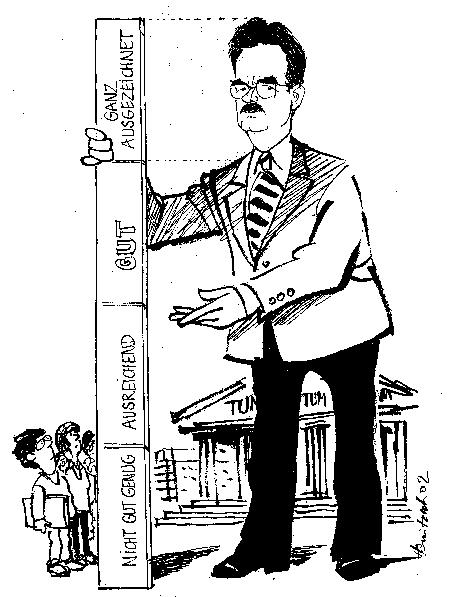
\includegraphics[width=0.8\textwidth]{\imgdir/steinberg.jpg}
\end{center}
\section{Studienfinanzierung}
\subsection{BAföG}
Das Bundesausbildungsförderungsgesetz (BAföG) ist den meisten wahrscheinlich bekannt. Es ist eine staatlich finanzierte Beihilfe für Studierende, deren Höhe abhängig von eurem und dem Einkommen eurer Eltern berechnet wird. Der Höchstsatz liegt bei knapp 600~\euro pro Monat, zusätzlich gibt es Zuschüsse zur Krankenversicherung, Auslandssemester u. Ä.. Ein Antrag lohnt sich auf jeden Fall, denn verlieren könnt ihr nichts - im schlimmsten Fall bekommt ihr bescheinigt,
dass euch aufgrund eurer finanziellen Situation keine staatliche Beihilfe zusteht. Informationen zum Antrag findet ihr auf der Webseite \url{www.studentenwerkfrankfurt.de}.

\subsection{Stipendien}
Eine gute Alternative zu BAföG, die viel weniger bekannt ist, sind Stipendien. In Deutschland gibt es 13 staatlich finanzierte Förderwerke und zahlreiche private Stiftungen, die Studierende finanziell und ideell fördern: Die Höhe der Geldförderung bei staatlichen Förderwerken unterliegt
auch dem Bundesausbildungsförderungsgesetz, zusätzlich bekommt ihr aber unabhängig vom Elterneinkommen 300~\euro Büchergeld. Unter ideeller Förderung versteht man Seminare und Sommerschulen, die die Förderwerke für ihre Stipendiaten organisieren. Was ihr im Gegenzug erbringen müsst, sind gute Leistungen im Studium (Achtung, lasst euch nicht abschrecken
– das heißt nicht, dass unbedingt eine 1 vor dem Komma stehen muss!!) und soziales/politisches/gesellschaftliches Engagement. Dazu zählen zum Beispiel aktive Mitarbeit in der
Schülervertretung oder einem gemeinnützigen Verein, wobei auch die persönlichen Umstände berücksichtigt werden. Ein weiterer Vorteil: Das Stipendium müsst ihr am Ende des Studiums
nicht zurückzahlen. Ausführliche Informationen über die 13 staatlichen Förderwerke findet ihr unter \url{www.stipendiumplus.de}. 

Neben diesen großen Förderwerken gibt es noch private Stiftungen, die Stipendien für verschiedenste Zwecke vergeben. Hier sind die Anforderungen
sehr unterschiedlich. Zum Beispiel gibt es Stipendien für soziale Projekte oder für Abschlussarbeiten
im bestimmten Bereich. Informationen hierzu findet ihr auf \url{www.mystipendium.de}.

Die Hürden sind in Wirklichkeit nicht so groß und die Stiftungen schöpfen ihre zur Verfügung stehenden Mittel oft gar nicht aus, deshalb lohnt sich ein Versuch!

\subsection{Studienkredit}
Alternativ gibt es noch die Möglichkeit, einen Studienkredit aufzunehmen. Zum Beispiel bietet die KfW Studienkredite zu günstigen Konditionen an. Für weitere Informationen schaut unter \url{www.studienkredite.org}.
\section{Studieren im Ausland}
\label{sec:Ausland}

Wie viele andere Studierende träumt ihr vielleicht auch davon, ein oder zwei Semester, vielleicht auch etwas länger, im Ausland zu verbringen.
Um euch einen Überblick über die verschiedenen Möglichkeiten und die Probleme, die man bei der Planung eines Auslandsaufenthalts hat, zu schaffen, haben wir für Euch ein paar Informationen gesammelt und hier zusammengestellt.
%
\subsection{Beste Zeitpunkte}
\begin{enumerate}
\item 3./4./5./6. Semester: möglich aber schwierig.
\item Die Bachelorarbeit im Ausland anfertigen -- dies machen nicht alle Professoren mit, bei Interesse müsst ihr Euern Jeweiligen fragen
\item 6./7./8. Semester: mit dem Beginn des Masterstudiums -- am entspanntesten.
\item Die Masterarbeit im Ausland anfertigen -- auch hier solltet ihr euern Betreuer/Professor ansprechen.
\end{enumerate}
%
\subsection{Vor- und Nachteile}
\begin{enumerate}
\item Im Bachelorstudium wird es schwierig(er) sein, sich die im Ausland erbrachten Leistungen anerkennen zu lassen, da durch das Bachelorstudium sehr genau festgelegt ist, welche Vorlesung mit welchem Inhalt wieviele Creditpoints erbringen soll. Wer darauf verzichten kann, in der Regelstudienzeit fertig zu werden, kann es aber versuchen und kann im schlimmsten Fall ein Studiensemester oder -jahr "`verlieren"'. Dafür lernst du aber schon sehr früh im Studium viel darüber, wie man sich auch in ungewohnten Umgebungen orientiert und wie es "`woanders läuft"'.
\item Die Bachelorarbeit im Ausland -- sofern möglich -- ist leider meistens relativ kurz ($\approx$ 3-5 Monate). Außerdem hat man sehr genaue Vorgaben, was man machen muss. Um das (Wunsch-)Land selbst kennen zu lernen, bleibt meist nicht so viel Zeit.
\item Der Masterstudiengang bietet durch seine Flexibilität (im Modul "`Wahlpflicht"' kann man viel flexibler Vorlesungen einbringen) eher Möglichkeiten, Studienleistungen aus dem Ausland anerkennen zu lassen. Außerdem gibt es keinerlei Pflichtvorlesungen, an denen man die Zeit im Ausland ausrichten müsste.
\item Die Masterarbeit im Ausland -- auch hier gilt, wie bei der Bachelorarbeit, dass evtl. wenig Zeit bleibt, das neue Land kennen zu lernen. Dafür ist die Masterarbeit -- in der Regel $\frac{1}{2}$ Jahr Einarbeitung + $\frac{1}{2}$ Jahr schreiben = 1 Jahr -- länger und bietet dadurch eher mehr Zeit.
\end{enumerate}
%
\subsection{Woher Informationen?}
Für eigentlich alle Angelegenheiten ist das "`International Office"' im Westend der geeignete Ansprechpartner.
Informationen findest du unter http://www.uni-frankfurt.de/international/ oder in der Sprechstunde des International Office. Eine Übersicht über die Sprechstunden findest Du auf der Internetseite.
%
\subsection{Wie geht das eigentlich?}
Generell gibt es drei Möglichkeiten:
\begin{enumerate}
\item Erasmus: Alle Länder der Europäischen Union sowie Beitrittskandidaten und einige weitere Länder (bspw. Schweiz, Norwegen) nehmen am Erasmus-Programm teil. Welche Universitäten für dich in Frage kommen, findest du auf der Homepage des International Office.
\item nicht-Erasmus: Für fast alle anderen Länder gibt es Förderprogramme des DAAD (Deutscher Akademischer AustauschDienst) -- diese Förderprogramme sind in der Regel höher dotiert als Erasmus, aber auch etwas schwieriger zu bekommen.
\item Alles auf eingene Faust: Du kannst natürlich einfach alles selbst machen -- vergibst damit aber wahrscheinlich die Chance auf ein Auslandsstipendium nach Erasmus oder DAAD (Ausnahme: evtl. "`Auslands-Bafög"'). Dafür kannst du im Prinzip, wohin du willst.
\end{enumerate}
%
\subsection{Wann sollte man sich Gedanken machen?}
Grundsätzlich sollte man sich etwa anderthalb Jahre vor dem geplanten Auslandsaufenthalt schon mal erkundigen.
Etwa ein Jahr vorher kann man sich dann anmelden, hat dann auch für alles noch genug Zeit.
Generell kann man nichts zu früh machen!
Wer zuerst kommt, bekommt die Plätze -- wer also spät oder spontan noch "`mal eben schnell"' ins Ausland will,
hat entweder keine große Auswahl oder gar keine Chance mehr auf einen Platz.
Im Zweifel gilt aber immer: Mutige vor!
Es soll auch Leute geben, die ihr Auslandssemester in ein paar Wochen organisiert haben\ldots
erzählt es nur nicht den Leuten im International Office ;-)
%
\subsection{Warum überhaupt?}
Da ihr ja eben erst an der Uni angekommen seid, macht es wohl mehr Sinn, über die dritte Variante, einen Auslandsaufenthalt nach dem Bachelor, nachzudenken.
Dabei sollte man sich darüber klar werden, warum man das machen möchte.
Denn über das "`Warum"' wird auch die Wahl des "`Wos"' leichter.
Eins ist jedoch klar: Es wird euer Studium nicht beschleunigen, bestenfalls ist man genau so schnell.
Dem Verfasser dieser Zeilen ist jedoch kein Student und keine Studentin bekannt, die ihr Auslandssemester oder -jahr bereut hat -- ganz im Gegenteil.
In der Physik gibt es zwar keinen besonderen Grund, aus Lehrgründen in bestimmte Länder zu gehen,
weil dort "`eine andere Art Physik"' gelehrt wird -- wie das vielleicht bei Philosophie oder Politik möglich sein kann.
Der eigentliche Grund wird daher eher "`Erweiterung des geistigen Horizonts"'
oder -- simpler ausgedrückt -- Spaß sein.
Wahrscheinlich wird man nie wieder in seinem Leben so viel Zeit haben, soviele interessante Leute aus der ganzen Welt kennenlernen und gemeinsam ein fremdes Land entdecken können.
Ob man nun ins kalte Wasser (Irlands, Norwegens, Polens oder Estlands) springt, die Sprache nicht kann
und versucht, gerade so irgendwelche Vorlesungen zu verstehen -- oder ins warme Wasser (Südspaniens, Italiens, Kroatiens, Griechenlands oder Bulgariens) springt,
schon aus Schulzeiten fließend die Landessprache spricht und schneller Kontakte knüpfen kann:
es wird sehr wahrscheinlich eine großartige Zeit sein, in der ihr viel Spaß haben könnt.
Sie wird sehr wahrscheinlich das Bild des Landes, in dem ihr studiert, verändern;
man lernt unheimlich viele Dinge, die keine Universität lehrt --
und man bekommt auch einen anderen Blick auf "`Zuhause"'.
Ganz abgesehen davon macht sich das ganze natürlich im Lebenslauf super...
%
\subsection{Was kostet es?}
\paragraph{USA} An den Top-Unis der USA muss man mit bis zu 22.000,-- \euro{} (3 Nullen!) für ein akademisches Jahr (ca. 9 Monate) rechnen. Es gibt allerdings kleinere Unis, die sich nach Studierenden aus dem Ausland förmlich reißen, um für einen besseren Ruf zu sorgen. Sie verlangen teilweise keine Tests und Studiengebühren. Fragt sich halt, ob man dort hin möchte. An den "`normalen"' Unis kann man sich aber absolut nicht darauf verlassen, finanziell in irgendeiner Art unterstützt zu werden. Es ist ratsam, einige Unis (z.B. per E-Mail) anzuschreiben und um Informationsmaterial für die Graduate-Studiengänge zu bitten. Das Amerikahaus veranstaltet übrigens gelegentlich Informationsabende zu diesem Thema.

\paragraph{Europa} In Europa dagegen sieht die ganze Sache schon besser aus: Wenn man mit Erasmus auf Entdeckungsreise geht, werden einem die evtl. anfallenden Studiengebühren erlassen. Dazu gibt es ein kleines Stipendium (2011: 150 \euro{}/Monat). Die Höhe des Stipendiums hängt jedoch empfindlich von der Anzahl der AuslandsstudentInnen ab. Darüber hinaus braucht man dann entsprechend das Geld, das im jeweiligen Land zum Leben reichen muss. Skandinavien und die Schweiz sind da tendenziell sehr viel teurer als Deutschland, Osteuropa eher etwas billiger und daher auch vor Ort "`leicher zu entdecken"'.

\paragraph{Rest der Welt} Es soll ja noch mehr als nur die USA und Europa geben: im Rest der Welt gibt es natürlich auch Unis! Dort ist der ganze Austauschprozess jedoch normalerweise nicht so sehr institutionalisiert wie in Europa, es gibt bspw. kein Erasmus. Der DAAD (siehe auch oben) hilft einem da aber finanziell und organisatorisch. Die Kosten hängen dort sehr stark davon ab, ob man die Studiengebühren "`weg-verhandeln"' kann und wie hoch die Lebenshaltungskosten des Landes sind. Auf der Homepage des DAAD gibt es eine Liste zu Fördersätzen und Reisekostenzuschüssen. Hier ist beinahe jedes Land, das mindestens eine Universität hat, möglich.

\subsection{Leistungen}
Auch hier sollte man sich sicherheitshalber vorher gründlich informieren.
Nicht alle Leistungsnachweise einer Uni im Ausland werden zu Hause anerkannt,
eventuell merkt man dann erst später, dass man das ein oder andere hier noch einmal machen muss.
Mit den neuen internationalen Bachelor- und Master-Studiengängen ist es auch innerhalb Europas nicht einfacher geworden.
Sprecht vorher mit dem entsprechenden Koordinator oder der Koordinatorin.
Dazu sucht ihr euch am besten schon einmal die Liste alle möglichen Vorlesungen heraus.
%
\subsection{Sprachtests}
\paragraph{USA und England}
In den USA und in England ist es die Regel, dass man bei der Anmeldung sein TOEFL-Ergebnis vorlegen muss.
TOEFL (Test Of English as a Foreign Language) ist ein Sprachtest, bei dem man Punkte bekommt.
Je besser, desto mehr Punkte.
Mit etwas Vorbereitung ist er allerdings gut zu schaffen.
An diesen Test sollte man früh genug denken, da es vom Abschicken der Anmeldung bis zum Test
und dann noch mal bis zur Punktebenachrichtigung 4-5 Monate dauern kann!
Das Ergebnis ist 2 Jahre lang gültig.

\paragraph{Rest der Welt}
Das International Office und auch der DAAD verlangen bei "verbreiteten Sprachen" --
Englisch, Spanisch, Französisch, evtl. mehr -- eine Bewerbung und ein Motivationsschreiben in Landessprache
sowie ein irgendwie gearteter Nachweis über Können der Landessprache.
Bei kleineren Ländern und weniger verbreiteten Sprachen --
z.B. Polnisch, Tschechisch, Bulgarisch, Portugiesisch, ... -- wird ein Motivationsschreiben in Englisch sowie ein kleiner -- an der Uni absolvierbarer -- Englisch-Sprachtest erwartet.

\subsection{Hinweis zum Schluss}
Da sich vieles mit den Austauschen im stetigen Wandel befindet, können die Informationen hier falsch, veraltet oder irreführend sein -- aktuell und hilfreich ist immer das International Office.
Schaut einfach unter http://www.uni-frankfurt.de/international/ nach, wann und wo sie ihre Sprechstunde haben -- und löchert sie dort mit Fragen.
Außerdem gibt es nicht so endlos viele Physikstudierende, die ins Ausland gehen, aber viele Programme.
Traut Euch und fragt -- Nur Mut! :-)
\von{Fips}
\newpage
\begin{figure}[!b]
	\centering
	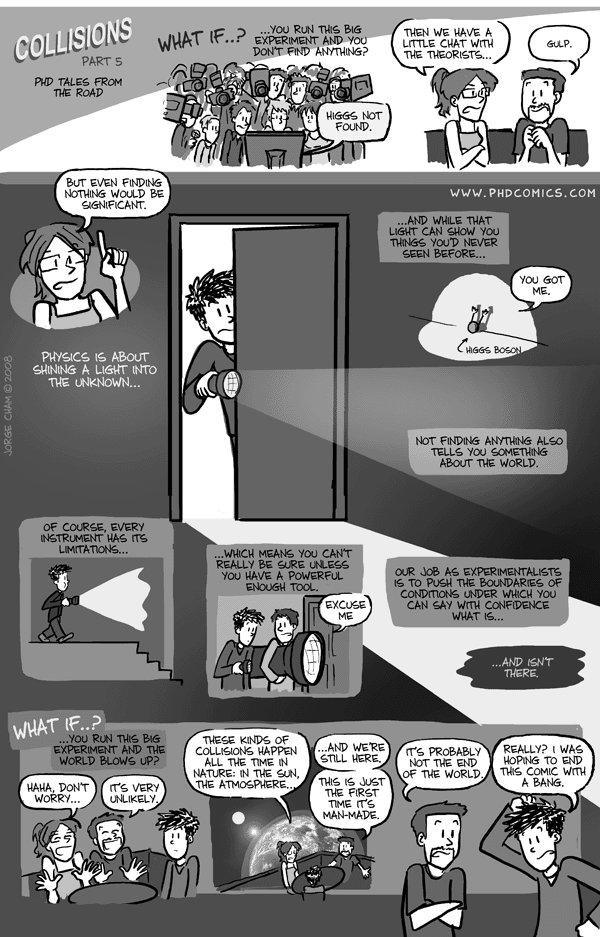
\includegraphics[height=\textheight]{\imgdir/cern.jpg}
\end{figure}

\section{Hochschulsport}

Ihr haltet euch für sportlich und auch relativ fit?\\
Tja, liebe Physikeinsteiger, verabschiedet euch von dieser Überzeugung, denn schon bald werdet ihr euren Hintern höchstens vom Bus in den Hörsaal, vom Hörsaal zum Tutorium und von dort ins Praktikum wuchten, wo ihr mit krummen Rücken über dem Schreiber der Triode kauert. \\
Wenn ihr dann nach einem 8-Stundentag nach Hause kommt, und eigentlich die doofen Matheübungen lösen solltet, habt ihr bestimmt keine Lust auf irgendeine Art von geistiger und körperlicher Betätigung.
So nimmt der körperliche Zerfall stetig zu.\\
Gerade deshalb solltet ihr euch bei mindestens einem Kurs des Hochschulsports anmelden.
Dort könnt ihr aus einem breiten Spektrum, von Afro--Dance bis Zen--Meditation, einen Kurs wählen, der euch geeignet erscheint.
Natürlich gibt es auch allgemeinpopuläre Sportarten.
Und das Beste ist:
Ihr seid ab nur fünf Euro pro Kurs und Semester dabei. \\
Dem besagten krummen Rücken könnt ihr zum Beispiel mit dem Kurs "`Rückenfit`` entgegenwirken.
Ihr meint, das ist nur was für Leute, die schon damals in der Schule wegen ihrer Wirbelsäulenfehlstellung gehänselt wurden?
Falsch gedacht würde ich meinen, denn nach kurzer Zeit ist die junge, wirklich hübsche Kursleiterin (die wahrscheinlich der Grund für die hohe Männerquote ist) von der netten schüchternen Dame zum Fitnesscoach mutiert, welcher euch mit hunderten Varianten von Sit-Ups traktiert, sodass ihr nicht wisst, ob der Schmerz im Bauch oder etwa der Druck in eurer Birne stärker ist.\\
Gegen den ständigen Input an neuen Informationen und die Reizüberflutung (z.B. in Mathe Satz von: Tonelli, Schwarz, Rolle,\ldots ) ist es auch mal nötig, sich einfach mal auf das "`Nichts`` zu konzentrieren.
Manche der Studienkollegen haben sich ihre natürlichen Schutzmechanismen wahrscheinlich schon frühzeitig während der Vorlesung selber angeeignet.
Jedoch ist für diejenigen, die noch immer die Stimme des Profs wahrnehmen, einer der Yoga-Kurse geeignet.
Hier lernt ihr nicht nur euren Kopf zu leeren, sondern auch, euch zu entspannen und euch beweglich zu halten.
An der "`Sportuni`` gibt es z.B. normales Hatha--Yoga und Power--Yoga. \\
Ich habe bisher nur von den mehr gesundheitsorientierten Sportarten berichtet, jedoch könnt ihr euch auch gerne in der Fitnesshalle allen guten Ratschlägen der Sportmedizinern widersetzen und einfach mal "`euren Body shapen`` (mehr oder weniger), denn wer braucht schon heile Gelenke wenn man Muckis hat?
Es kann dann natürlich passieren, dass kompetentes Fachpersonal eingreift und euch daran hindert noch mehr Gewichte aufzulegen.
Ein nettes Angebot für den weiblichen Teil der Schöpfung ist das "`Angeleitete Gerätetraining für Frauen``, welches wenig Stress verspricht. \\
Weitere Sportarten sind natürlich diverse Ballspiele (Rugby verspricht wahrscheinlich auch eine gute Anzahl von blauen Flecken), eine Reihe von Kampfsportarten, verschiedene Tanzarten, Leichtathletik usw\ldots \\
Ich bin eventuell nicht sonderlich repräsentativ, da ich nur seltsame Sachen wie Power-Yoga, Ballett, Allwetterlauf oder Rückenfit gemacht habe.
Aber ich habe auch von anderen fast nur Positives über den Hochschulsport gehört.
Die Lehrkräfte sind wirklich kompetent, verstehen was von ihrem Fach und sind meistens auch sehr nett.
Die Preise sind wie gesagt kaum zu unterbieten. \\
Ich kann deshalb jedem empfehlen, sich für mindestens einen Kurs anzumelden.
Ihr könnt die Kurse die ersten beiden Wochen ohne Anmeldung besuchen und so testen, was euch Spaß macht.\\
Das Programm erscheint in der Regel ca. zwei Wochen vor Vorlesungsbeginn, dies ist auch als E-Paper im Internet vorhanden.
Kleiner Rat am Rande: Geht nicht am ersten Anmeldungstag los, um euch anzumelden.
Denn in der Regel ist ein riesiger Haufen von Studenten da, die auch nicht davor scheuen, Gewalt anzuwenden um möglichst schnell einen Platz in einem der sehr beliebten Kurse zu bekommen.
Wollt ihr aber einen sehr populären Kurs besuchen, müsst ihr euch wohl oder übel ins Gefecht stürzen.
Ich weiß jedoch nicht, welche Kurse davon betroffen sind (Ballett für Fortgeschrittene höchstwahrscheinlich nicht ?).\\
Das aktuelle Programm der "`Sportuni"' findet ihr auf der Homepage des Zentrums für Hochschulsport unter \textbf{http://web.uni-frankfurt.de/hochschulsport/}.
Dort könnt ihr euch auch zu Beginn der Vorlesungszeit für die einzelnen Sportkurse anmelden.\\ 
Die meisten Kurse finden übrigens im \textbf{Zentrum für Hochschulsport, Ginnheimer Landstr. 39} statt.
Man erreicht es sehr bequem mit dem Bus 34 ("`Universitäts-Sportanlagen"') oder der Straßenbahn 16 ("`Frauenfriedenskirche"').
Dort liegt auch das Programmheft mit den allgemeinen organisatorischen Hinweisen aus.\\

Also dann, viel Spaß!
\von{Nata}
\begin{figure}[!h]
 \begin{center}
  
\includegraphics[height=3in]{bilder/thatsitkerl.jpg}
 \end{center}
\end{figure}

\section{Orientierung}
Bei der Orientierung auf dem Campus Riedberg geraten Studentenaus allen Semestern und Fachrichtungen regelmä\ss ig in Verzweiflung. Wo finde ich denn Raum \_ \_.111? Wie hei\ss t denn der gro\ss e Hörsaal?\\
Auf dem Riedberg gibt es mehere universtäre Gebäude, das gro\ss e, überaus hübsche, graue ist die Chemie, direkt daneben findet man die Unterkunft von Pharmazie und Biochemie. Dort findet sich auch die Mensa (das wichtigste in diesem Gebäude). Weiter in Richtung der U3 findet man ein gro\ss es rotes Gebäude: die neue Biologie. Au\ss erdem existiern zwei Backsteingebäude: In dem kleineren der beiden sind die Geowissenschaften beheimatet und das grö\ss ere ist das wichtigste für euch: Die Physik. Schräg gegenüber der Physik in Richtung der U8/U9 befindet sich das Infrastrukturzentrum mit Hörsäälen und der Bibliothek.
\vfil
\begin{figure}[h]
	\centering
    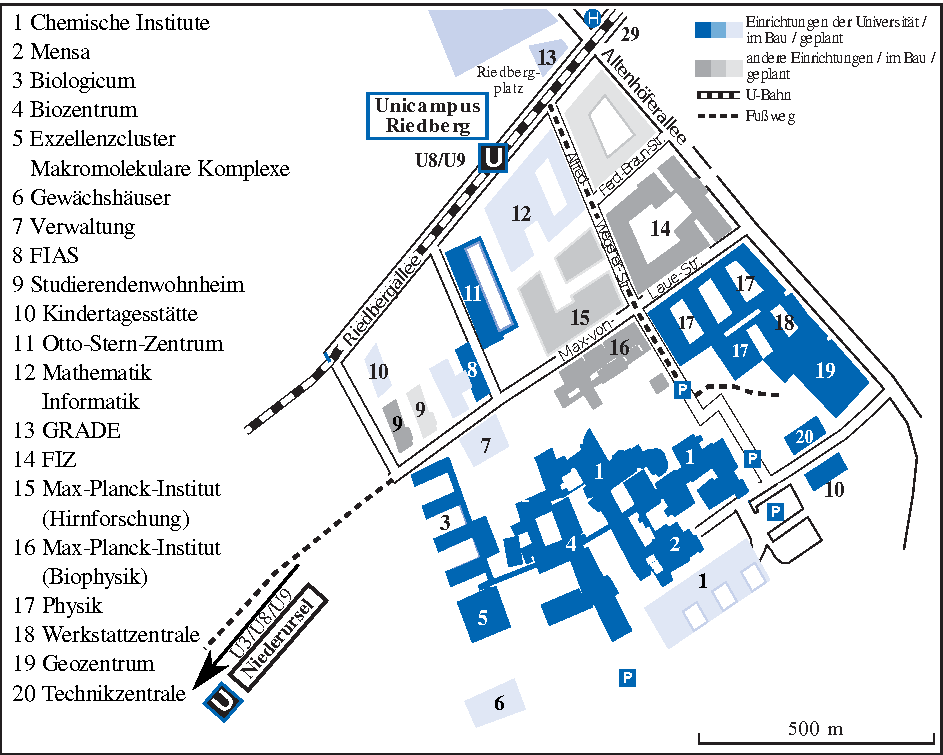
\includegraphics[width=0.80\textwidth]{\imgdir/riedberg-lageplan0.pdf}
\end{figure}
\newpage
Um euch eine komplette Beschreibung des Campus zu liefern, ist dieses Heft zu klein. Daher beschränke ich mich auf die Physik: Der Ort, an dem ihr die meiste Zeit eures Studiums lernen und arbeiten werdet.\\
Die Numerierung der Räume in unserem Gebäude ist zwar logisch, sorgt allerdings immer wieder für Verwirrungen. Jede Raumnummer besteht aus vier bis fünf Zahlen, wobei die hintern drei durch einen Punkt von den restlichen getrennt werden. Vor dem Punkt steht das Stockwerk. Das Erdgeschoss erhhält nicht wie zu erwarten eine 0 oder gar keine Bezeichnung, sondern zwei Unterstriche. Das Untergeschoss erkennt man an einem Unterstrich und einer 0 vor dem Punkt. Die anderen Stockwerke sind standartmä\ss ig bezeichnet (erster Stock: 1; zweiter Stock: 2). Die erste Zahl nach dem Punkt gibt das Gebäude an, die letzten beiden sind einfach die Raumnummer. Welches Gebäude welche Nummer hat, könnt ihr auf unserem Plan sehen.\\
Wenn man jetzt also den Raum \_ \_.208 sucht, dann muss man im Erdgeschoss in das zweite Gebäude gehen (beim Pförtner) und dort am Ende des Ganges findet man dann den Raum (das ist übrigens die Fachschaft).
\vfil
\begin{center}
    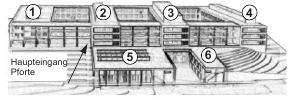
\includegraphics[width=1.00\textwidth]{\imgdir/plan.png}
\end{center}
\section{Bibliothek}

Die Bibliothek ist sehr wichtig für Studierende: 
Man findet dort Lehrbücher, Monographien und Journals die man zum Studium braucht.
In der Bibliothek Naturwissenschaften am Campus Riedberg könnt ihr
die Lehrbücher für Physik und Mathematik ausleihen,
aber auch die für die Fachbereiche Geowissenschaften, Biowissenschaften,
Biochemie, Chemie und Pharmazie.

Die Lehrbücher für die Grundvorlesungen (alle Pflichtmodule im Bachelor) sind in Semesterstärke vorhanden.
Das bedeutet, jeder Studierende kann ein Exemplar ausleihen
und bis Ende des Semesters behalten.
Diese Bücher sind extra gekennzeichnet -- mit einem grünen Aufkleber -- und können nur Mo-Fr 8:00-18:00 ausgeliehen werden.
Bücher aus der normalen Lehrbuchsammlung könnt Ihr ohne
Vorbestellung in Selbstbedienung ausleihen. 
Die Leihfrist beträgt 4 Wochen, eine Verlängerung ist nicht möglich.

Neben der Lehrbuchsammlung gibt es noch die sogenannte \glqq RVK\grqq  (Regensburger Verbundsklassifikation) Sammlung. Sie befindet sich weiter hinten in der Bibliothek und besteht aus Büchern zu spezielleren Themen, die über die normalen Lehrveranstaltungen hinausgehen. Hier findet ihr alles von Supersymmetrie bis Wolkenphysik oder Materialwissenschaften. Die Bücher in diesem Bereich sind alle nur in kleiner Stückzahl vorhanden (1-4). Meist gibt es zwei Exemplare, eins ist ausleihbar und eins ist Präsenzbestand sodass es immer vor Ort benutzt werden kann. Diese Bücher tragen ein großes gelbes Schild auf dem Buchrücken, auf denen \glqq nicht ausleihbar\grqq steht (ist klar, oder?). Die RVK-Sammlung wird für euch wahrscheinlich erst später im Studium interessant wenn ihr Spezialvorlesungen hört, in denen Profs mit Vorliebe ihr eigenes Buch als Literatur angeben oder wenn ihr spezielle Literatur für eure Abschlussarbeiten braucht. Klolektüre lässt sich hier auch gut finden. 
Die Bücher in dieser Sammlung sind ebenfalls ausleihbar für 4 Wochen, können allerdings bis zu 5 Mal um jeweils 4 Wochen verlängert werden, sofern es keine Vormerkung eines anderen Schwei... ähm Nutzers gibt.

Die dritte große Kategorie an Schriften in der Bibliothek sind die Zeitschriften. Weil sich das ein bisschen zu sehr nach Blitz-Illu und Bunte anhört nennen Wissenschaftler sie aber meistens Journals. Hier werden keine Kuchenrezepte und Diättipps veröffentlicht, sondern wissenschaftliche Abhandlungen, meistens \glqq paper\grqq genannt. Die Journals sind im oberen Stockwerk der Bibliothek zu finden und sind alphabetisch nach Titel sortiert. Hier kann man stundenlang nach dem richtigen suchen, da leider nicht immer nach dem ersten Wort des Titels sortiert wird. Droht ihr euch dort zu verlaufen, fragt einfach an der Theke nach. Die Bibliotheksmitarbeiter haben hier auch oft ihre Probleme aber mit etwas Glück, finden sie schneller, was ihr sucht. 
Zeitschriften sind generell nicht ausleihbar. Fast alle Journals gibt es auch online. Ihr könnt sie lesen falls die Uni ein Abo des passenden Journals hat. Hierzu müsst ihr euch mit eurem Bibliotheksaccount auf der Seite des Journals anmelden. Falls ihr keinen Zugang bekommt weil die Uni nicht genug an die Hu... vom Verlag zahlt gibt es eine hilfreiche Website, die wir euch natürlich nicht offiziell empfehlen dürfen. Nur so viel dazu. Sie fängt mit Sci an und hört mit hub auf, alles dazwischen müsst ihr selbst rausfinden.

Neben Büchern gibt es in der Bibliothek auch Gruppenarbeitsräume und einen Computerraum, in dem man arbeiten kann. Beide sind von der Bibliothek räumlich getrennt und auch außerhalb der Öffnungszeiten der Bibliothek geöffnet. Sie sind beide nur für Studierende geöffnet. Für die Gruppenarbeitsräume muss an der Theke der Bib ein Schlüssel ausgeliehen werden. Der Computerraum kann mit der Goethe-Card geöffnet werden.

Du belegst als Nebenfach Sozialwissenschaften, brauchst das eine Buch aus der Zentralbibliothek aber an der UBahn wird mal wieder gebaut und du hast wirklich gar keinen Bock, mit dem Ersatzbus bis nach Bockenheim zu fahren? Bücher aus der Zentralbibliothek können in (fast) jeden Standort der Bib bestellt und dann abgeholt werden. Auch wenn ihr ein Buch aus der BNat in einer anderen Bibliothek abgeben möchtet ist das kein Problem. Auch hier gilt: Man kann Bücher aus fast jeder Bibliothek in fast jeder anderen abgeben. Schwierig wird es immer wenn es sich um folgende Bibliotheken handelt: Mathe, Informatik, Sport.

Falls ein Prof ein Buch empfiehlt, das absolut klausurrelevant und unerlässlich ist, das die Bib aber nicht besitzt oder das es nicht am Riedberg gibt, keine Panik. Du musst nicht direkt die 5 Euro, die nach Miete noch von deinem Bafög übrig sind sparen, um dieses Buch zu kaufen. Es gibt auf der Website der Bibliothek den Kaufvorschlag. Die Bibliothek ist immer dankbar für Vorschläge und fast alles, was vorgeschlagen wird, wird auch zeitnah angeschafft. Solange es halbwegs sinnvoll ist. Ihr bekommt eine Nachricht sobald das Buch verfügbar ist und es wird direkt für euch reserviert. Ihr könnt es dann einfach an der Theke abholen und euer restliches Bafög in Schokolade anlegen.

Solltest du ein Buch zu spät abgegeben haben, macht die Uni leider direkt Auge. die Gebühren sind bei $\frac{3 Euro}{Buch*Woche}$ und können an der Theke bezahlt werden (\textbf{nur bis 18:00 Uhr}). Bei 12 Euro Schulden bei der Bib oder mehr könnt ihr erstmal keine neuen Bücher mehr ausleihen. Ganz wichtig ist: wenn ihr ein Buch abgebt werden die Mahngebühren eingefroren. Ihr könnt sie einfach später zahlen. Wenn ihr das aber zu lange nicht macht ($\geq 6 Monate$) wird ebenfalls eure Goethe Card für Ausleihen gesperrt, auch wenn ihr weniger als 12 Euro offen habt. Wir empfehlen immer, die Gebühren an der Theke zu zahlen (nur in Bar und \textbf{bis 18:00 Uhr}), da es bei der Überweisung viel Zeit in Anspruch nimmt bis sie an der richtigen Stelle verbucht wird. \par

Das war meine (Janika, Fachschaftlerin und Hiwi in der Bibliothek) kleine schriftliche Bibliotheksführung. Am Anfang des Semesters veranstaltet die Bibliothek aber immer \glqq richtige echte \grqq Führungen. Es empfiehlt sich sehr, so eine Führung mitzumachen. Dort bekommt ihr nochmal alles ganz genau gezeigt, ihr lernt die Räumlichkeiten und das Bibliothekspersonal kennen und ihr könnt Fragen stellen. Außerdem lernt ihr, wie man die Website der Bibliothek benutzt und wie man im Bibliothekssystem Recherchen durchführt, das ist nämlich nicht ganz trivial.
Aber das wichtigste was ihr euch immer merken solltet: \textbf{DIE SEMESTERAUSLEIHE UND MAHNGEBÜHREN BEZAHLEN GEHT NUR BIS 18:00 UHR!!!11!!elf!}



\begin{minipage}{0.5\textwidth}
\noindent
\textbf{Öffnungszeiten:}\\\\
Montag - Freitag 08.00 - 20.00 Uhr\\
Samstag 10.00 - 16.00 Uhr\\


\noindent
\textbf{Ausleihzeiten Semesterausleihe und Mahngebühren:}\\
Montag - Freitag  08.00 - 18.00 Uhr\\


\noindent
\textbf{Öffnungszeiten der Gruppenarbeitsräume:}\\
Montag - Freitag  08.00 - 22.30 Uhr\\
Samstag und Sonntag 10.00 - 19.00 Uhr\\


\noindent
\textbf{Internetadressen:} 
\begin{itemize}
   \item{Bibliothek Naturwissenschaften:}\\
    http://www.ub.uni-frankfurt.de/bnat/home.html
   \item{Universitätsbibliothek:}\\
      http://www.ub.uni-frankfurt.de/
\end{itemize}

\end{minipage}
\begin{minipage}{0.5\textwidth}
 \begin{center}
  %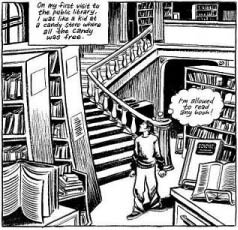
\includegraphics[height=7 cm]{bilder/manga.jpg}
  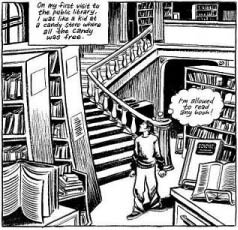
\includegraphics[height=7 cm]{bilder/manga.jpg}
\end{center}
%\vspace*{4cm}
\end{minipage}
\von{Margret}


\section{Der Gleichstellungsrat Physik}
Der Gleichstellungsrat Physik hei\ss t alle Erstsemester herzlich willkommen an der Goethe-Universität Frankfurt.\\
Der Gleichstellungsrat Physik setzt sich im Moment aus sieben gewählten
Frauen zusammen. Sie vertreten die Statusgruppen der Studentinnen, der
wissenschaftlichen und technisch-administrativen Mitarbeiterinnen und
der Professorinnen. Diese werden, je nach Statusgruppe, alle ein bis zwei Jahre von der Frauenvollversammlung der Physik gewählt. Die nächste Wahl findet übrigens im kommenden Frühjahr statt.\\
Wir setzen uns für die Themen Chancengleichheit und Familienförderung ein und unterstützen Studierende und Mitarbeiter/innen in allen Lebenslagen. Au\ss erdem engagieren wir uns für viele spannende Projekte wie den Girls' Day oder die Lunch Talks der technisch-administrativen Mitarbeiter/innen. Wir unterstützen die Teilnahme an verschiedenen Tagungen, zum Beispiel der Deutschen Physikerinnentagung oder der Zusammenkunft aller Physik-Fachschaften (ZaPF). Unsere ausleihbare Spielkiste hat schon manchem Elternteil, das spontan sein Kind mit zur Arbeit bringen musste, den Tag gerettet.\\
Speziell für euch Erstsemester bieten wir das Mentoringprogramm Ersti-Hilfe an. Jeder Mentee wird dabei ein Semester lang von einer Kommilitonin oder einem Kommilitonen aus den höheren Semestern durch das Studium begleitet. So können zum Beispiel Fragen zum Zeitmanagement geklärt werden, es gibt viele Tipps und Tricks für das Studium und ihr gewinnt im besten Fall einen Ansprechpartner für eure gesamte Studienzeit. Anmeldung per formloser E-Mail an \url{ersti-hilfe@physik.uni-frankfurt.de}.\\
Weitere Informationen, unsere Kontaktdaten und wie man bei uns mitmachen kann, findet ihr auf unserer Webpage \url{http://goethe.link/gsr-physik}.\\
Wir wünschen euch viel Erfolg im Studium und hoffen, euch bald kennenzulernen!\\
\von{Euer Gleichstellungsrat Physik}

\includegraphics[width=0.5\textwidth]{\imgdir/ersti-hilfe.png}
\section{Kleines Physiker--Überlebens--ABC}


\begin{description}
    \item[Amt für Ausbildungsförderung:] Hier kannst du BAFöG-Formulare
abholen und in ausgefüllter Form wieder abgeben.

    \item[Assistent:] Die
netten (seltener auch nicht netten) Menschen, die in den Praktika
eure Praktikumsprotokolle durchsehen und dann mit der Aufschrift
"`ok"' zurückgeben (oder auch nicht).

    \item[AStA:]Allgemeiner Studierenden Ausschuss.
      Vom \textbf{Stu}dierenden\textbf{pa}rlament gewählt, sozusagen die Regierung desselben.
      Im StuPa tummeln sich die Nachwuchspolitiker
      (Grüne Hochschulgruppe, Juso-Hochschulgruppe, Giraffen - Unabhängige Fachbereichsgruppen,
      RCDS - Ring Christlich-Demokratischer Studenten, Schildkröten, LHG - Liberale Hochschulgruppe,
      attac/independent students, Die Linke.SDS, Pinguine, LiLi - Wahlbündnis Linke Liste,
      DL - Demokratische Linke Liste, FDH - Fachschafteninitiative Demokratische Hochschule)
      und investieren jedes Jahr 500.000 \euro{} für die Studierenden.

    \item[Auslandsstudium:]Wer Interesse an einem Auslandsstudium hat, kann sich bei der Studienberatung
      und beim DAAD informieren.
      Mehr Informationen dazu auch im Kapitel Auslandsstudium (Seite \pageref{sec:Ausland}).

    \item[Ausschüsse:]Der \textbf{F}ach\textbf{b}ereichs\textbf{r}at setzt
verschiedene Ausschüsse ein: So die QSL-Kommision, Prüfungsausschüsse für die einzelnen Studiengänge
und den Studienausschuss.
In allen Ausschüssen sitzen Studierende, die versuchen, die Interessen ihrer Kommiliton(in)en zu
vertreten.

    \item[Bachelor:]Unterste Physikerweihe und seit neuestem auch
berufsqualifizierend. Wird nach sechs Semestern gemacht.

\begin{figure}[!h]
\begin{center}
  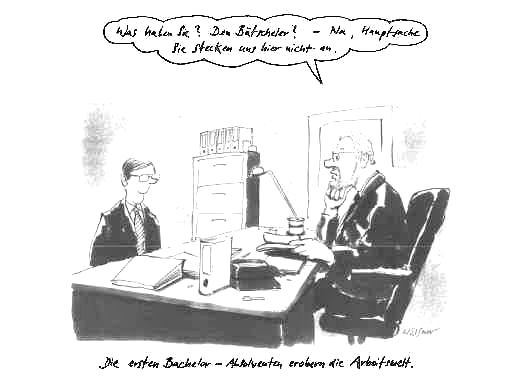
\includegraphics[width=.8\textwidth]{bilder/bachelor.jpg}
\end{center}
\end{figure}

    \item[Bafög:]Bundes-Ausbildungs-Förderungsgesetz.
      Möglichkeit für Studierende, deren Eltern nicht allzuviel verdienen, ein paar Euro
Unterstützung zum Studieren zu bekommen.
Wer meint, dafür in Frage zu kommen, sollte auf jeden Fall einen Antrag beim Amt für
Ausbildungsförderung im Sozialzentrum stellen.
Verlieren kann man nicht viel, nur gewinnen\ldots oder man kriegt nix.

\item[Café Physik:] Eine gute Alternative zur Mensa.
  Mit hübschem Ausblick über die Experimentierhalle.

\item[Campi:] Standorte der Uni.
  Offiziell haben wir momentan 4 + einen Sportcampus.

   \item[Credit Points:] Die Leistungseinheit der neusten Ideen der Bildungsminister:
     Ein Credit Point (CP) stellt angeblich 30 Stunden Arbeitsaufwand für den durchschnittlichen Studierenden dar.
Dieser durchschnittliche Studierende ist allerdings Russe, hat eine Uhr,
auf der zwischen zwei Sonnenaufgängen nur vier Stunden vergehen und nimmt regelmäßig Speed.
In einem Semester solltet ihr etwa 30 CPs sammeln, für den Bachelor müsst ihr 180, für den
Master weitere 120 CPs nachweisen.

    \item[c.t:] "`Cum tempore"': die Veranstaltung beginnt erst nach der "`akademischen`` Viertelstunde.

    \item[Dekan:] Professor, der vom Fachbereichsrat gewählt wird, um ihn nach außen zu vertreten.
      Im Moment ist Prof.Philpsen Dekan des FB13.

    \item[Dekanat:]Verwaltung des Fachbereichs.
      Dem Dekan unterstellt.
      Direkt um die Ecke bei der Fachschaft.

    \item[Didaktik:] Mancher hat sie drauf und mancher halt nicht.
      Auch die Kurzform für das Institut Didaktik der Physik.

    \item[Diplom:] Der Abschluss des Diplomstudiengangs (ist für euch aber sowieso relativ
uninteressant, weil ihr auf BaMa studiert).

    \item[Doppelstudium:]Theoretisch ist es möglich, neben Physik noch ein anderes Fach
(z.B. Mathe oder Philosophie) zu studieren -- L3-ler haben immer
zwei Fächer, allerdings nicht im gleichen Umfang wie Diplom,
Magister oder BaMastudierende. Bei einem Doppelstudiengang sind zeitliche
Kollisionen unvermeidlich und mehr Arbeit ist es natürlich auch.
Dennoch kann man es versuchen; man kann das zweite Fach ja
fallenlassen.

    \item[Dr.h.c:] Doktortitel ehrenhalber (so was wie Helmut
Kohl mal hatte). Um einen Doktortitel führen zu dürfen, muss man
was leisten. Das ist normalerweise eine eigenständige
Forschungsarbeit in der Form der Doktorarbeit. Wenn ein Forscher
(in der Regel ein Prof) für die Wissenschaft in einem Gebiet
herausragendes geleistet hat, kann es passieren, dass eine
Universität diesem Forscher einen Ehrendoktortitel verleiht, mit
dem sich der Ausgezeichnete zusätzlich schmücken darf. Passiert
dies einem Forscher mehrmals (multus, z.B. dem alten Greiner aus der Theorie), darf er sich Prof
Dr.Dr.h.c.mult nennen.

\item[Erstis:] Ihr... und alle anderen, die sich auch noch in höheren Semestern so fühlen.

    \item[Fachschaft:]Die netten Leute, die für
euch diese Handbroschüre und diese Einführungsveranstaltung gemacht
haben. Laut HHG (Hessisches Hochschulgesetz) bilden eigentlich
alle Studierende des Fachbereichs die Fachschaft. Umgangssprachlich
bezeichnet man aber mit "`Fachschaft`` die Gruppe der Studierenden, die
sich für die Interessen der Studierenden am Fachbereich einsetzt. In der
Fachschaft kann man Physikstudierende aus allen Semestern
kennenlernen, die einem auch mal Tipps fürs eigene Studium geben
können. Die Fachschaft sucht ständig neue Leute, also schaut
einfach einmal bei einem Fachschaftstreffen vorbei.

    \item[Fachschaftsrat:]Die Studierenden eines Fachbereiches wählen im
Wintersemester u.a. den Fachbereichsrat. Die gewählten
Studierendenvertreter (und nur die) dürfen offiziell im Namen der
Fachschaft sprechen und Geld ausgeben. In anderen Fachbereichen
läuft das so: Da kandidieren von den hochschulpolitischen
Gruppen der Parteien Vertreter auf eigenen Listen und der
Fachbereichsrat besteht am Ende z.B. 2 Leuten von den Grünen,1
Juso und 2 vom RCDS. Diese liegen sich dann ständig in den Haaren,
weil sie alle nur Parteipolitik machen. Zum Glück sind wir so
wenige und man ist sich einig.

    \item[Fachbereich:]Der Fachbereich (FB)
ist eine nach fachlichen Gesichtspunkten eingegrenzte
Organisationseinheit der Uni. Früher hieß so etwas Fakultät. Es
gibt an der Uni Frankfurt insgesammt 16 FB. Interessant sind für
euch aber hauptsächlich nur FB11 Geowissenschaften, FB12
Mathematik und Informatik, FB13 (der tollste FB überhaupt), FB14
Chemie und FB15 Biologie.

    \item[Fachsbereichsrat:]Trifft sich regelmäßig und bespricht
alles, was den Fachbereich irgendwie angeht, besteht aus Profs,
Studierenden, wissenschaftlichen Mitarbeitern und
administrativ-technischem Personal.

    \item[Freizeit:] Was ist denn das?

\item[Goethe--Card:] Bekommt ihr, wenn ihr sie nicht schon habt, im StudierendenServiceCenter in Bockenheim.
Sie ist gleichzeitig Studierendenausweis, RMV-Ticket, Bibliotheksausweis, Eintrittskarte für den Palmengarten und ihr könnt damit in der Mensa bezahlen.

\item[Greiner, Walter:]
Ist der berühmteste Professor der letzten Zeit aus Frankfurt und
hat zu Alledem noch die roten "`Physikbibeln`` geschrieben.

    \item[Harri Deutsch:] Verlag aus Frankfurt, der auch einige Physikb\"ucher im Programm hat.

    \item[HiWis:] Hilfswissenschaftler, Sklaven der Professoren.

    \item[HRZ:]Hochschulrechenzentrum, das sind die Leute, die euch nen Account
geben und mit denen ihr euch rumschlagt (oder sie mit euch), wenn
der Computer mal spinnt.

    \item[Institute:]Da gibt es zum einen das
Physikalische Institut, das Institut für Theoretische Physik, die
Angewandte Physik, Kernphysik, Biophysik sowie das Institut für Didaktik der Physik.

    \item[Internet:]Beliebtes
Mittel, um beispielsweise Protokolle auszutauschen.\\
www.fachschaft.physik.uni-frankfurt.de ist auch dafür eine
tolle Adresse im Netz.

    \item[Klausur:] In Physik werden euch mit dem BaMa-Studiengang
wahrscheinlich des öfteren mal Klausuren begegnen.
Normalerweise benötigt ihr nur 50\% der erreichbaren Punkte um zu bestehen und
wenn das nicht klappt, könnt ihr es nochmal versuchen\ldots oder Pech
gehabt.

    \item[Klopfen:] Komische Tradition nach der Vorlesung. Wird
wahrscheinlich gemacht, um die Leute zu wecken.

    \item[Kolloquium:]Eigentlich mündliche Prüfung bei Professor oder Assistent.
    Dann gibt es noch das physikalische Kolloquium, eine Veranstaltung mittwochsabends.
Da reden dann auswärtige Wissenschaftler über ihre aktuelle Forschung.
Man versteht oft rein gar nichts, es ist aber trotzdem empfehlenswert, hinzugehen!

    \item[Kommilitonen:] Eure Mitstudierenden.

\item[Linguisten:] Haben was mit Sprache und Verständnis zu tun, interessieren uns also nicht.

\item[Master:] Hört sich an wie bei Konfuzius, ist es auch fast.
Wenn ihr den habt, seid ihr schon fast weise.

    \item[Mathevorlesung:]Dienstag und Donnerstag von 8-10.
 Meist der Graus aller neuen Physiker, doch es
ist durchaus zu schaffen und eigentlich nicht uninteressant.
Blüht euch aber erst im Wintersemester.

    \item[Mensa:]Je mehr der Speiseplan verspricht, desto mehr Vorsicht!

\begin{figure}[!h]
 \begin{center}
  
\includegraphics[width=\textwidth]{bilder/yes.jpg}
 \end{center}
\end{figure}

\item[Modul:]
Wie ein Puzzleteil\ldots Ihr müsst viele sammeln und richtig zusammen stecken, dann
kommt ein Abschluss dabei raus.

    \item[Nebenfach:]Notwendiges Übel oder Spaß.
    Das liegt meist an der Wahl des Nebenfaches.

    \item[Physikerinnen:]Aufstrebende Gattung, die diese Männerdomäne immer mehr überollt.
    Ihr dürft sie auch ansprechen ;)

    \item[Praktikum:] Eigentlich:"`Physikalisches Anfängerpraktikum Teil I und Teil II``.
Spielstunde am Nachmittag, in der es um Mechanik/Thermodynamik/Optik (Teil I) bzw.
Elektrodynamik (Teil II) geht. Zusätzlich zum Experimentieren
wollen Protokolle geschrieben werden (Übel).

    \item[Präsident:]Selbstklärend, oder?

    \item[Prof. emeritus:]Professor, der eigentlich schon
im Ruhestand ist, aber trotzdem noch im Institut rumgurkt.

    \item[Promotion:] Erhebung auf ein höheres Level.
    Wer promoviert hat, darf sich ein Dr. vor den Namen klatschen.

\item[Psychologische Beratung:] Braucht ihr, nachdem ihr das Studierendensekreteriat verlassen habt.

    \item[Regelstudienzeit:]Für euch sechs Semester (bis zum Bachelor)\ldots

    \item[s.t.:]"`Sine tempore``: bist du
nicht zur gegebenen Zeit da, brauchst du ne gute Ausrede.

    \item[Scheine:]Genau wie mit dem Geld: "`sammeln und drauf aufpassen``.
    Für eure Bachelorprüfung braucht ihr diverse Modulzertifikate.
In der Physik musst du für die Scheine regelmäßig vorrechnen und Aufgaben
abgeben.

    \item[Semesterferien:]\ldots gibt's nicht.
    Nur eine vorlesungsfreie Zeit.
In dieser Zeit muss man für die Klausuren (ja, die finden alle in den "`Ferien`` statt)
lernen und kann Blockpraktika machen oder einfach nur faulenzen. In höheren Semestern
wird man auch in dieser Zeit an der Uni arbeiten, z.B. an der
Abschlussarbeit.

    \item[Semesterticket:]Eine der praktischsten Erfindungen
seit geschnittenem Brot! Eure Fahrkarte für das gesammte RMV-Netz,
nie wieder wird man so billig die öffentlichen Verkehrsmittel
nutzen können!!

    \item[Seminar:]Veranstaltung, in der
Vorträge gehalten werden. Gibt es einen Schein für das Seminar,
muss man im Normalfall auch selbst einen halten.

    \item[Senat:]Ist die zentrale Vertretung aller Statusgruppen der Universität.

    \item[Sozialzentrum:]Das Gebäude, in dem sich u.a. Studierendensekretariat, Mensa und
BaFöG-Amt (genauer: Amt für Ausbildungsförderung) befinden.

    \item[Sport:]Empfehlenswert, gerade das Zentrum für Hochschulsport (ZfH) bietet coole Kurse an!

    \item[Stipendien:]Wer gute Schul-/Studienleistungen vorzuweisen hat,
sollte sich um ein Stipendium bemühen.
Selbst vorschlagen kann man sich mitlerweile bei allen zwölf staatlichen Stiftungen.
Das sind die parteinahen (Konrad-Adenauer-Stiftung
(CDU-nah), Friedrich-Ebert-Stiftung (SPD-nah),
Friedrich-Nauman-Stiftung (FDP-nah), Heinrich-Böll-Stiftung
(Grüne-nah) und Rosa-Luxemburg-Stiftung (Linke-nah)),
die kirchlichen Stiftungen (Cusanuswerk (katholisch), Studienwerk Villigst (evangelisch)
und das Ernst Ludwig Ehrlich Studienwerk (jüdisch)),
die Stiftung der Deutschen Wirtschaft und die Studienstiftung des Deutschen Volkes.
Neben den Studienleistungen spielt bei allen Stiftungen auch
gesellschaftliches, soziales, politisches und/oder kirchliches
Engagement eine Rolle.
Nähere Informationen zu Stipendien gibt es in der zentralen Studienberatung.
Bewerben lohnt sich auf jeden Fall!!

    \item[Studierendensekretariat:]Unter der Mensa in Bockenheim,
dort kann man sich rückmelden und allerlei Bescheinigungskram
bekommen, vor Allem aber stundenlang anstehen, um mit überaus netten und zuvorkommenden
Menschen zu diskutieren, wenn mal nicht alles so klappt, wie man will.

    \item[Studierendenenwerk:] Die netten Leute, die uns z.B. in der Mensa
mit Essen versorgen.

    \item[Studienberatung:]Machen Prof. Wagner und Prof. Roskos (für Physik),
, Prof. Mäntele (für Biophysik),
    Prof. Engel (für Computational Science) und Frau Korneck und Herr Ritter
    (für Lehramt).
Helfen bei allen Fragen, die beim
Studium so auftauchen können ("`Bin ich denn wahnsinnig?"',
"`Warum tue ich mir denn das alles an?"').
%Beklagen sich manchmal über zu wenig Arbeit.
%Zu finden in Gebäudeteil 4 ganz unten.
%Aber auch wir sind immer f\"ur Fragen offen.

\begin{center}
    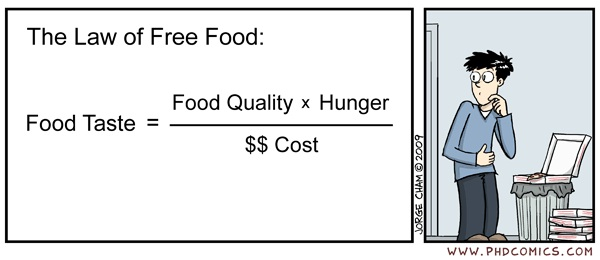
\includegraphics[width=.9\textwidth]{bilder/food.jpg}
\end{center}

\item[Studiengebühren:] Haben wir zum Gl\"uck nicht mehr.
ABER man kann nie wissen.
Also seid achtsam!

\item[Thai:] Imbiss gegen\"uber der Bushaltestelle.
Wen das Mensaessen nicht krank gemacht hat, kann sein Gl\"uck hier versuchen.

 \item[Theoretikum:]Übungen in der Theoretischen Physik, wie Praktikum, nur
theoretisch.

    \item[Tutor:] Das sind Studierende höherer Semester, die eure
Übungsgruppen betreuen und eure Aufgaben korrigieren.
Freuen sich, wenn ihr sie mit Fragen löchert.

    \item[Übungen:]
Zum einen die kleinen, gemeinen Zettel, die ihr wöchentlich bekommt.
Dann gibt es aber auch die Übungsstunde, in denen die Dinger dann besprochen werden.

%    \item[Volkssternwarte:] Oben im physikalischen Verein, Freitags gibts da
%Vorträge und Sterne gucken kann man auch. Der Eingang ist übrigens
%an der Rückseite des alten Physikgebäudes in Bockenheim.

    \item[Wahlen:]Du darfst im Wintersemester wählen.
    Und du sollst es auch, denn die
Demokratie lebt vom Mitmachen und dir ist doch die Demokratie
lieber als die Diktatur, oder etwa nicht? Schliesse dich also der
wählenden Minderheit an\ldots ansonsten wird dem AStA das Geld
gekürzt und die können dann nicht mehr so viel machen, wie z.B.
für euer Semesterticket kämpfen.
Im Einzelnen wählst du
Fachschaftsrat und Fachbereichsrat (Physik-intern) sowie
Studierendenparlament und den Senat (Uni-weit).

    \item[WiWis:]Wirtschaftswissenschaftler.
    Der Fachbereich mit den meisten Studierenden (über 4000).
 Sitzt am Westend.
 Wird von manchen als Erzfeind angesehen, für diese
Bezeichnung eignen sich die Mathematiker aber wesentlich besser.

\item[Zentralmensa:]In Bockenheim.
Seid froh, dass ihr da nicht essen müsst.

%\begin{center}
%    
\includegraphics[width=1.00\textwidth]{bilder/ansehen.jpg}
%\end{center}

\end{description}
%
%\begin{figure}[!h]
% \begin{center}
%  \includegraphics[height=\textheight]{bilder/phd.jpg}
% \end{center}
%\end{figure}

\section{Programm der Einführungsveranstaltung}

\bigskip

\begin{centering}
\renewcommand{\arraystretch}{1.5}
\begin{tabular}{|p{1.5cm}||p{8cm}  |p{5cm}|}
  \hline
  \multicolumn{3}{|l|}{\textbf{Dienstag, 03.04.15}}				\\ \hline
  Zeit	& Programm					& Ort			\\ \hline
  9:00	& Physikalische Einführung	 & Hörsaal Physik (\_ 0.111)		\\ \hline
  10:00	& Vorstellung Fachschaft	& Hörsaal Physik (\_ 0.111)		\\ \hline
  10:30	& Rallye			& 	\\ \hline
  13:00	& Mittagessen		& Mensa	\ $\pi \times$Gaumen		\\ \hline
  14:00	& Uniformalitäten & 	Biologicum Poolraum \ (0.405) \\ \hline		
  15:00	& Professorencafé 		& Hilbertraum (02.116) 		\\ \hline
  16:30	& Studiengangsvorstellung & Hörsaal Physik (\_ 0.111) 		\\ \hline
  18:30 & Abendessen 			&	Hilbertraum (02.116) 		\\ \hline
  20:00 & Abendprogrammm	        &	 \\ \hline
\end{tabular}
\end{centering}

\begin{centering}
\renewcommand{\arraystretch}{1.5}
\begin{tabular}{|p{1.5cm}||p{8cm}  |p{5cm}|}
  \hline  
  \multicolumn{3}{|l|}{\textbf{Mittwoch, 04.04.15}} 			\\ \hline
  09:00 & Nebenfach-Frühstück & Hilbertraum (02.116) \\ \hline
  10:30 & Bibiliotheksvortrag & Hörsaal Physik (\_ 0.111) \\ \hline
  11:30 & Vorstellung Anfängerpraktikum & \_\_.206 und \_\_.207 \\ \hline
  12:30 & Überaschung & Hof \\ \hline
   	
\end{tabular}
\end{centering}


\section{Autoren}

%\markboth{Impressum}
%p{1.5cm}||p{8cm}  |p{5cm}
\begin{tabular}{p{3.5cm}p{6cm}p{6cm}}
\textbf{Herausgeber:} 	& Fachschaft Physik Frankfurt\\
						& Goethe Universität \\
						& Max-von-Laue Str. 1\\
						& 60438 Frankfurt \\
						&				\\
\textbf{Chefredakteure:} &Eva Katharina Rafeld & (WiSe05-WiSe10)\\
			 			 &Fritz Kretzschmar & (WiSe05-WiSe07)\\
			 			 &Gunnar Gräf & (WiSe05)\\
			 			 &Patricia Till & (WiSe07-WiSe10)\\
			 			 &Sophia Henneberg & (SoSe11)\\
			 			 &Margret Heinze & (SoSe11-WiSe12/13)\\
			  			 &Virginia Britten & (SoSe13)\\
			  			 &Miriam Weller & (SoSe11-WiSe14/15)\\
			 			 &Julia Sammet & (SoSe15-Wise 2017/2018)\\
			 			 &Nils Köhne & (SoSe18)\\\\
\textbf{Autoren:}	& Bj\o rn Bäuchle 		& Viola Bennert \\
					& Thomas Burschil 		& Fiona Faber \\
					& Julia Fischbach 		& Margarita Gorodezky\\
					& Janina Hesse    		& Luisa Ickes\\
					& Daniela Kern-Michler  & Kristin Kliemt\\
					& Berit Körbitzer		& Fritz Kretzschmar\\
					& Frederike Kubandt		& Marco Marquardt\\
					& Renate Märtin			& Jenny Muraschko\\	
					& Alex Mayr				& Jonas Rist\\
					& Fips Schneider		& Martin Sprenger\\							& Christian Stuck		& Patricia Till	\\							& Sascha Vogel			& Ole Hinrichs\\		
					&						& 			\\	
					& Prof. Rischke & Prof. Wagner\\
					& Prof. Reifarth & Dr. Jarohs \\
					&				&			\\	
\end{tabular}

\begin{tabular}{p{3cm}p{13cm}}

\textbf{Bilder:} 	& Julia Fischbach \& Patricia Till  \\
					&									\\
\textbf{Layout:} &Bj\o rn Bäuchle, Fritz Kretzschmar, Daniela Kern-Michler \\ 
&  Satz: \LaTeXe  \\
\end{tabular}

% hier die Seitenanzahl anpassen, um auf ein Vielfaches von 4 zu kommen
\section*{Notizseiten}
\cleardoubleevenpage 

\pagestyle{empty}
\newpage
\begin{figure}[!b]
\begin{center}
  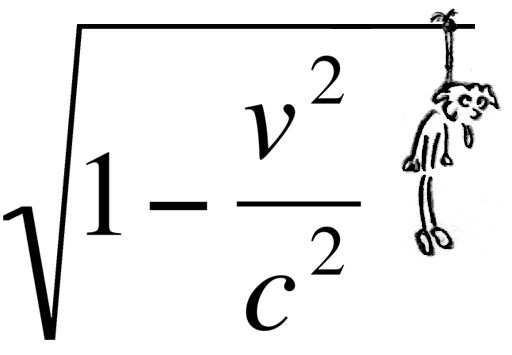
\includegraphics[width=\textwidth]{bilder/erhaengt.jpg}
\end{center}
\end{figure}
